% This template originates from the Cambridge University thesis 
% which is created by Prof Harish Bhanderi.  
% This is template follows the GNU license for Education and training
% purposes. (http://www-h.eng.cam.ac.uk/help/tpl/textprocessing/ThesisStyle/) 
%
% Modified by Toan Ha Van - toanhv.vietnam@gmail.com
% The Academy of Cryptography Techniques, Vietnam
% 04/05/2017
%

\documentclass[oneside]{Classes/KMA}

% pdfmetadata: However, if you are using the hyperref package (which uses your Table of Contents to create bookmarks and a contents pane in your PDF - very pretty) you will find your pdfinfo block is ignored.
% \ifpdf 
%     \pdfinfo { /Title  (Research about Methodologies of Intrusion Detection for WiFi Networks)
%                /Creator (TeX)
%                /Producer (pdfTeX)
%                /Author (Toan Ha Van - toanhv.vietnam@gmail.com)
%                /CreationDate (D:20170303031010)  %format D:YYYYMMDDhhmmss
%                /ModDate (D:20170606031010)
%                /Subject (Research about Methodologies of Intrusion Detection for WiFi Networks)
%                /Keywords (WiFi Security; Wireless Intrusion Detection System; WiFi Access Point; Opensource Software; Kismet Wireless; OpenWrt)}
%     \pdfcatalog { /PageMode (/UseOutlines)
%                   /OpenAction (fitbh)  }
% \fi

\university{{BAN CƠ YẾU CHÍNH PHỦ}}%
\collegeordept{{HỌC VIỆN KỸ THUẬT MẬT MÃ}}%
% standard temple does not include logo
\crest{
\includegraphics[scale=0.45]{kmalogo.png}}%
\title{NGHIÊN~CỨU~CÁC~PHƯƠNG~PHÁP~PHÁT~HIỆN XÂM~NHẬP\\MẠNG~WIFI}%
\supervisor{{TS. Nguyễn~Anh~Tuấn}}%
\supervisororg{{Trường Đại học Công nghệ Thông tin}}%
\supervisororgext{{Đại học Quốc gia TP. Hồ Chí Minh}}%
\author{{Hà~Văn~Toàn}}%
\grade{{9}}%
\class{{AT9D}}%
\major{{Công~nghệ~thông~tin}}%
\submajor{{An~toàn~thông~tin}}%
\majorcode{{52.48.02.01}}%
\degreedate{TP.~Hồ Chí Minh,~2017}%
\hbadness=10000
\hfuzz=50pt
\usepackage{StyleFiles/watermark}
\onehalfspacing

% begin: format source code
\definecolor{dkgreen}{rgb}{0,0.6,0}
\definecolor{gray}{rgb}{0.5,0.5,0.5}
\definecolor{mauve}{rgb}{0.58,0,0.82}
\lstset{
    frame=single,
    language=c,
    aboveskip=2mm,
    belowskip=2mm,
    showstringspaces=false,
    columns=flexible,
    basicstyle={\footnotesize\ttfamily},
    numbers=none, 
    keywordstyle={\color{blue}},
    commentstyle={\color{dkgreen}},
    stringstyle={\color{mauve}},
    breaklines=true,
    breakatwhitespace=true,
    tabsize=2
}
% end: format source code

\renewcommand{\baselinestretch}{1.3}
\begin{document}
% change geometry to resize bolder of cover
\newgeometry{a4paper,left=3cm,right=2.5cm,top=2cm,bottom=2.5cm}
\makecover%
\makebackcover%
% restore geometry defaults
\restoregeometry%
%\newgeometry{a4paper,left=3.5cm,right=2cm,top=3cm,bottom=3cm}
\setcounter{secnumdepth}{3}
\setcounter{tocdepth}{3}
%
\frontmatter % book mode only
\pagenumbering{roman}
% 
\begin{dedication}  
\fontsize{14pt}{21pt}\selectfont

Xin dành tặng quyển luận văn này cho ... 

\end{dedication}

 
\begin{acknowledgements}
Tôi muốn bày tỏ sự biết ơn sâu sắc và chân thành đến Thầy giáo TS. Nguyễn~Anh~Tuấn, Thầy đã tận tình hướng dẫn và tạo mọi điều kiện cho tôi trong quá trình tìm hiểu, nghiên cứu và thực hiện đồ án tốt nghiệp. Sự tận tình và nhiệt huyết của Thầy là nguồn động lực dồi dào, thúc đẩy tôi không ngừng nỗ lực để hoàn thành đồ án một cách tốt nhất.

Tôi xin gửi lời cảm ơn đến các giảng viên đang công tác tại Học~viện~Kỹ thuật~Mật~mã. Các Thầy Cô đã dạy bảo, chỉ dẫn và luôn tạo điều kiện tốt nhất cho tôi trong suốt quá trình học tập và nghiên cứu tại học viện.

Con xin dành lời cảm ơn to lớn nhất đến bố, mẹ và gia đình. Bố, mẹ và gia đình đã luôn ở bên con, là nguồn động lực không mệt mỏi và là chỗ dựa tinh thần vững chắc giúp con vượt qua những khó khăn để hoàn thành tốt đồ án này.

Mặc dù đã nỗ lực cố gắng song đồ án này chắc chắn không thể tránh khỏi sai sót, khuyết điểm. Tôi kính mong nhận được sự thông cảm và tận tình chỉ bảo, góp ý của quý Thầy Cô và các bạn.

\begin{flushright}
    Tp. Hồ~Chí~Minh, ngày 04 tháng 05 năm 2017

    {\textbf{Sinh viên thực hiện}\hspace*{1.25cm}\par}
    \vspace*{1cm}
    \textbf{Hà~Văn~Toàn}\hspace*{2cm}
\end{flushright}
\end{acknowledgements}
  
\begin{commitments}
Tôi xin cam đoan bản đồ án này do tôi tự nghiên cứu dưới sự hướng dẫn của Thầy giáo TS. Nguyễn~Anh~Tuấn.


Để hoàn thành đồ án này, tôi chỉ sử dụng những tài liệu đã ghi trong mục tài liệu tham khảo, ngoài ra không sử dụng bất cứ tài liệu nào khác mà không được ghi.


Nếu sai, tôi xin chịu mọi hình thức kỷ luật theo quy định của học viện.

\begin{flushright}
    Tp. Hồ~Chí~Minh, ngày 04 tháng 05 năm 2017

    {\textbf{Sinh viên thực hiện}\hspace*{1.25cm}\par}
    \vspace*{3.5cm}
    \textbf{Hà~Văn~Toàn}\hspace*{2cm}
\end{flushright}
\end{commitments}
  
%
\tableofcontents
\chapter*{DANH MỤC TỪ VIẾT TẮT}
\addcontentsline{toc}{chapter}{DANH MỤC TỪ VIẾT TẮT}

\begin{table}[H]
\centering
\small
\setlength{\extrarowheight}{1pt}
\begin{tabular}{|l|p{6cm}|p{7cm}|}
\hline
\multicolumn{1}{|c|}{\textbf{Từ}} & \multicolumn{1}{c|}{\textbf{Viết tắt của}}                              & \multicolumn{1}{c|}{\textbf{Ý nghĩa}}                        \\ \hline
AME                               & AirMagnet Enterprise Server                                             & Máy chủ trong giải pháp AirMagnet Enterprise                 \\ \hline
AP                                & Access Point                                                            & Điểm truy cập                                                \\ \hline
ATIM                              & Announcement Traffic Indication Message                                 & Khung thông báo chỉ dẫn lưu thông                            \\ \hline
BSS                               & Basic Service Set                                                       & Tập dịch vụ cơ bản                                           \\ \hline
BSSID                             & Basic Service Set Identifier                                            & Định danh tập dịch vụ cơ bản                                 \\ \hline
BPF                               & Berkeley Packet Filter                                                  & Cú pháp lọc gói BPF                                          \\ \hline
CCMP                              & Counter Mode Cipher Block Chaining Message Authentication Code Protocol & Giao thức xác thực thông điệp sử dụng mã khối chế độ CTR-CBC \\ \hline
CUWN                              & Cisco Unified Wireless Network                                          & Giải pháp an ninh hợp nhất cho mạng không dây của Cisco      \\ \hline
DMZ                               & Demilitarized Zone                                                      & Vùng mạng trung lập                                          \\ \hline
EAP                               & Extensible Authentication Protocol                                      & Giao thức xác thực mở rộng                                   \\ \hline
ESS                               & Extended Service Set                                                    & Tập dịch vụ mở rộng                                          \\ \hline
ESSID                             & Extended Service Set Identifier                                         & Định danh tập dịch vụ mở rộng                                \\ \hline
HIDS                              & Host-based Intrusion Detection System                                   & Hệ thống phát hiện xâm nhập máy chủ                          \\ \hline
IDS                               & Intrusion Detection System                                              & Hệ thống phát hiện xâm nhập                                  \\ \hline
IEEE                              & Institute of Electrical and Electronics Engineers                       & Viện Kỹ thuật Điện và Điện tử                         \\ \hline
IETF                              & Internet Engineering Task Force                                         & Một cơ quan phát hành chuẩn Internet                         \\ \hline
IPS                               & Intrusion Prevention System                                             & Hệ thống ngăn chặn xâm nhập                                  \\ \hline
LLC                               & Logical Link Control                                                    & Lớp con điều khiển liên kết luận lý                          \\ \hline
MAC                               & Media Access Control                                                    & Lớp con kiểm soát truy cập thiết bị                          \\ \hline
MITM                              & Man-in-the-middle                                                       & Tấn công chặn bắt thông tin                                  \\ \hline
NIDS                              & Network-based Intrusion Detection System                                & Hệ thống phát hiện xâm nhập mạng                             \\ \hline
NIST                              & National Institute of Standards and Technology                          & Viện Tiêu chuẩn và Công nghệ Quốc gia (Hoa Kỳ)               \\ \hline
\end{tabular}
\end{table}

\begin{table}[H]
\centering
\small
\setlength{\extrarowheight}{1pt}
\begin{tabular}{|l|p{6cm}|p{7cm}|}
\hline
OSI                               & Open Systems Interconnection                                            & Mô hình tham chiếu OSI                                       \\ \hline
RAP                               & Rogue Access Point                                                      & Điểm truy cập giả mạo                                        \\ \hline
RFC                               & Request for Comments                                                    & Các chuẩn được duyệt bởi IETF                                \\ \hline
SIEM                              & Security Information and Event Management                               & Hệ thống quản lý sự kiện an ninh                             \\ \hline
SMTP                              & Simple Mail Transfer Protocol                                           & Giao thức truyền thư đơn giản                                \\ \hline
SNMP                              & Simple Network Management Protocol                                      & Giao thức quản lý mạng đơn giản                              \\ \hline
SSID                              & Service Set Identifier                                                  & Định danh tập dịch vụ                                        \\ \hline
STA                               & Station                                                                 & Trạm                                                         \\ \hline
TKIP                              & Temporal Key Integrity Protocol                                         & Giao thức toàn vẹn khóa tạm thời                            \\ \hline
VLAN                              & Virtual Local Area Network                                              & Mạng cục bộ ảo                                               \\ \hline
WCS                               & Wireless Control System                                                 & Thành phần quản lý tập trung trong CUWN                      \\ \hline
WEP                               & Wired Equivalent Privacy                                                & Chuẩn mã hóa WEP                                             \\ \hline
WiFi                              & Wireless Fidelity                                                       & Mạng không dây theo chuẩn 802.11                             \\ \hline
WIDS                              & Wireless Intrusion Detection System                                     & Hệ thống phát hiện xâm nhập mạng không dây                   \\ \hline
WIPS                              & Wireless Intrusion Prevention System                                    & Hệ thống ngăn chặn xâm nhập mạng không dây                   \\ \hline
wIPS                              & Adaptive Wireless Intrusion Prevention System                           & Hệ thống ngăn chặn xâm nhập của CUWN                         \\ \hline
WLC                               & Wireless LAN controller                                                 & Hệ thống phát hiện xâm nhập mạng không dây của CUWN          \\ \hline
WPA                               & Wi-Fi Protected Access                                                  & Chuẩn mã hóa WPA                                             \\ \hline
WPA2                              & Wi-Fi Protected Access II                                               & Chuẩn mã hóa WPA2                                            \\ \hline
WPS                               & Wi-Fi Protected Setup                                                   & Giao thức xác thực đơn giản của thiết bị Access Point        \\ \hline
\end{tabular}
\end{table}

  
\listoffigures
  %\printnomenclature
  %\addcontentsline{toc}{chapter}{Nomenclature}
\listoftables

\mainmatter
%\chapter*{TÓM TẮT}
%\addcontentsline{toc}{chapter}{TÓM TĂT}
%\begin{abstract}
Tóm tắt luận văn. Tóm tắt luận văn. Tóm tắt luận văn. Tóm tắt luận văn. Tóm tắt luận văn. Tóm tắt luận văn. Tóm tắt luận văn. Tóm tắt luận văn. Tóm tắt luận văn. Tóm tắt luận văn. Tóm tắt luận văn. Tóm tắt luận văn. Tóm tắt luận văn. Tóm tắt luận văn. Tóm tắt luận văn. Tóm tắt luận văn. Tóm tắt luận văn. Tóm tắt luận văn. 

Tóm tắt luận văn. Tóm tắt luận văn. Tóm tắt luận văn. Tóm tắt luận văn. Tóm tắt luận văn. Tóm tắt luận văn. Tóm tắt luận văn. Tóm tắt luận văn. 

Tóm tắt luận văn. Tóm tắt luận văn. Tóm tắt luận văn. Tóm tắt luận văn. Tóm tắt luận văn. Tóm tắt luận văn. Tóm tắt luận văn. Tóm tắt luận văn. Tóm tắt luận văn. Tóm tắt luận văn. Tóm tắt luận văn. Tóm tắt luận văn. Tóm tắt luận văn. Tóm tắt luận văn. Tóm tắt luận văn. Tóm tắt luận văn. 
%\end{abstract}

\chapter*{MỞ ĐẦU}
\addcontentsline{toc}{chapter}{MỞ ĐẦU}
%\begin{preface}
Theo một báo cáo đầu năm 2017~\cite{kemp2017digital}, Việt Nam hiện có hơn 49 triệu người dùng Internet, là một trong những quốc gia có tỷ lệ người dùng Internet cao nhất trên thế giới. Trong đó, đa phần là người dùng sử dụng các thiết bị thông minh như máy tính xách tay, điện thoại thông minh, máy tính bảng và Internet TV. Cùng với sự phát triển của Internet, mạng WiFi cũng dần thay thế cho mạng có dây truyền thống. Mạng WiFi có mặt ở khắp mọi nơi, từ các nơi công cộng như sân bay, khách sạn, quán cà phê đến các hộ gia đình. Mạng WiFi mang lại những lợi ích rõ rệt, nó giúp cho việc truyền tải, tiếp nhận thông tin cực kỳ nhanh chóng và tiện lợi, giúp người sử dụng công nghệ tiết kiệm thời gian, nâng cao hiệu quả công việc~\cite{Khan2017}.

Bên cạnh những lợi ích như vậy, mạng WiFi vẫn tồn tại những vấn đề khiến người dùng lo lắng, như ảnh hưởng của sóng WiFi đối với sức khỏe con người (mặc dù chưa có bằng chứng khoa học nào chính thức đề cập~\cite{foster2013wi}), hay nguy cơ mất an toàn thông tin trong mạng. Nguy cơ mất an toàn thông tin trong mạng WiFi hiện đang là vấn đề rất cấp thiết, cần có sự phối hợp giải quyết của cả tổ chức quản lý hạ tầng mạng và người dùng. Hiện nay trên thế giới đã có nhiều giải pháp giúp phát hiện sớm các cuộc tấn công trong mạng WiFi, tạo ra các cảnh báo tới nhà quản trị và thậm chí có thể ngăn chặn cuộc tấn công đang diễn ra~\cite{karen2015comparing}. Tuy nhiên, hầu hết chúng đều là các giải pháp dành cho doanh nghiệp lớn, cần chi phí đầu tư lớn cho một hạ tầng mạng WiFi hoàn chỉnh.

Với ý tưởng phục vụ cho đối tượng là doanh nghiệp nhỏ, quán cà phê và hộ gia đình, đồ án này sẽ nghiên cứu các giải pháp sẵn có, từ đó xây dựng một hệ thống phát hiện xâm nhập mạng WiFi dựa trên các phần mềm mã nguồn mở. Hệ thống này có thể tích hợp dễ dàng lên hạ tầng thiết bị thông thường, người dùng có thể sở hữu một hệ thống phát hiện xâm nhập mạng WiFi với các tính năng an toàn, giao diện quản lý thân thiện, chỉ với chi phí rất thấp.\\

Do thời gian nghiên cứu còn hạn chế, báo cáo này không thể tránh khỏi một số sai sót, khuyết điểm. Tác giả kính mong quý Thầy, Cô và các bạn đóng góp ý kiến để đồ án hoàn thiện và thực tiễn hơn. Xin chân thành cảm ơn!

\begin{flushright}
    Tp. Hồ~Chí~Minh, ngày 04 tháng 05 năm 2017

    {\textbf{Sinh viên thực hiện}\hspace*{1.25cm}\par}
    \vspace*{1cm}
    \textbf{Hà~Văn~Toàn}\hspace*{2cm}
\end{flushright}
%\end{preface}

% \pagebreak[4]%
% \hspace*{1cm}%
% \pagebreak[4]%
% \hspace*{1cm}%
% \pagebreak[4]%

\chapter{GIỚI THIỆU ĐỀ TÀI}

\ifpdf
    \graphicspath{{Chapter1/Chapter1Figs/PNG/}{Chapter1/Chapter1Figs/PDF/}{Chapter1/Chapter1Figs/}}
\else
    \graphicspath{{Chapter1/Chapter1Figs/EPS/}{Chapter1/Chapter1Figs/}}
\fi

\section{Tên đề tài}
Nghiên cứu các phương pháp phát hiện xâm nhập mạng WiFi.

\section{Từ khóa}
WiFi Security - Bảo mật mạng WiFi, Wireless Intrusion Detection System - Hệ thống phát hiện xâm nhập mạng không dây, WiFi Access Point - Điểm truy cập WiFi, Opensource Software - Phần mềm mã nguồn mở, Kismet Wireless, Snort, OpenWrt.

\section{Nội dung và giới hạn của đề tài}

\subsection{Nội dung của đề tài}
Hệ thống phát hiện xâm nhập là một giải pháp bảo mật đang được ứng dụng rộng rãi trong các hệ thống của các tổ chức. Tuy nhiên, chúng chủ yếu được dùng để bảo vệ các máy chủ và mạng có dây, vấn đề phát hiện xâm nhập trong mạng WiFi chưa được quan tâm đúng mức. Ngoài ra, chi phí về giá thành cũng như vấn đề triển khai khá phức tạp của các giải pháp hiện có, làm cho chúng không phù hợp với các tổ chức và doanh nghiệp nhỏ tại Việt Nam. Mục tiêu của đề tài là nghiên cứu về các phương pháp phát hiện xâm nhập mạng WiFi, các hệ thống hiện có, từ đó ứng dụng các phần mềm mã nguồn mở để xây dựng một hệ thống phát hiện xâm nhập cho mạng WiFi, với các tính năng bảo mật và chi phí hợp lý. Cụ thể đề tài thực hiện những mục tiêu sau:

\begin{itemize}
\item Tìm hiểu những kiến thức nền tảng về mạng WiFi, để hiểu rõ các mô hình mạng và hoạt động. Từ đó chỉ ra những điểm yếu và các tấn công điển hình trong mạng WiFi.
\item Nghiên cứu về các phương pháp phát hiện xâm nhập phổ biến, và những đặc điểm riêng của phát hiện xâm nhập trong mạng WiFi.
\item Khảo sát về các hệ thống phát hiện xâm nhập mạng WiFi hiện có, phân tích ưu nhược điểm.
\item Tìm hiểu về các phần mềm phát hiện xâm nhập mã nguồn mở và các phần mềm liên quan.
\item Tìm hiểu về thiết bị Access Point, quá trình xây dựng một firmware OpenWrt và thay thế firmware có sẵn của thiết bị.
\item Tìm hiểu về máy tính nhúng Raspberry Pi và ứng dụng của nó.
\item Từ những kiến thức trên, xây dựng một hệ thống phát hiện xâm nhập mạng WiFi để thử nghiệm, đánh giá.
\end{itemize}

\subsection{Giới hạn của đề tài}
Các nguy cơ gây mất an toàn thông tin trong mạng WiFi rất đa dạng. Cùng với đó, các kỹ thuật phát hiện xâm nhập cũng không ngừng cải tiến để bảo vệ hệ thống. Đây là một chủ đề khá rộng, đề tài này chỉ tập trung vào một số tấn công điển hình trong mạng WiFi, hệ thống phát hiện xâm nhập được hiện thực chỉ có tính năng phát hiện xâm nhập và đưa ra cảnh báo, chưa có tính năng chặn đứng các tấn công ngay khi nó diễn ra. Tuy nhiên với việc sử dụng các phần mềm mã nguồn mở và đang được tiếp tục phát triển bởi cộng đồng, hệ thống này có khả năng mở rộng rất lớn.

Đề tài cũng không bao gồm các kiến thức về lớp vật lý của mạng WiFi, hay các tấn công trên lớp vật lý như tấn công phá sóng. Các hệ thống phát hiện xâm nhập hiện có hầu hết cũng chưa thể giải quyết các vấn đề này.\\ \\ \\ \\

\section{Cấu trúc báo cáo}
Báo cáo đồ án được cấu trúc như sau:

Chương 1 giới thiệu tổng quan về đề tài nghiên cứu, mục đích nghiên cứu, phạm vi nghiên cứu của đề tài.

Chương 2 cho thấy các nguy cơ gây mất an toàn thông tin thường trực trong mạng WiFi. Từ đó, nghiên cứu về hệ thống phát hiện xâm nhập, các phương pháp phát hiện xâm nhập để phát hiện và đưa ra các cảnh báo kịp thời khi xảy ra các cuộc tấn công. Đồng thời, chương này cũng đi khảo sát các hệ thống đã được phát triển, khái quát các kiến thức, công nghệ liên quan.

Chương 3 đưa ra hướng tiếp cận của đề tài, từ đó cụ thể thiết kế hệ thống và phân tích các luồng hoạt động.

Chương 4 trình bày việc hiện thực các thiết kế từ chương 3, giới thiệu giao diện quản lý hệ thống. Cuối chương là kiểm thử và đánh giá hệ thống được xây dựng.

Cuối cùng, đề tài được tổng kết trong chương 5, nêu lên ý nghĩa và đưa ra hướng phát triển tiếp theo.

\chapter{KIẾN THỨC NỀN TẢNG VÀ KHẢO SÁT}
\ifpdf
    \graphicspath{{Chapter2/Chapter2Figs/PNG/}{Chapter2/Chapter2Figs/PDF/}{Chapter2/Chapter2Figs/}}
\else
    \graphicspath{{Chapter2/Chapter2Figs/EPS/}{Chapter2/Chapter2Figs/}}
\fi

Để có thể thực hiện được những mục tiêu cụ thể đã đề ra trong chương đầu tiên, chương này đồ án sẽ trình bày về các kiến thức nền tảng cho việc xây dựng đề tài, đồng thời cũng thực hiện khảo sát các hệ thống, phần mềm có liên quan.

Đầu tiên đồ án sẽ nói về các kiến thức cơ bản về mạng WiFi như định nghĩa, các mô hình mạng, các loại khung và các tiêu chuẩn mã hóa. Tiếp theo là các tấn công điển hình trong mạng WiFi, chúng có đặc điểm gì và vì sao có thể phát hiện được các tấn công đó đang diễn ra. Kế tiếp là tổng quan về hệ thống phát hiện xâm nhập, từ đó tìm hiểu sự khác nhau giữa hệ thống phát hiện xâm nhập thông thường và hệ thống phát hiện xâm nhập cho mạng WiFi (hay mạng không dây). Cuối chương đồ án sẽ khảo sát về các hệ thống phát hiện xâm nhập đã được phát triển và các kiến thức liên quan để phục vụ cho việc thiết kế hệ thống WIDS đề xuất ở chương sau.

\section{Tổng quan về mạng WiFi}

\subsection{Giới thiệu}
\emph{WiFi} là tên rút gọn của Wireless Fidelity, dùng để chỉ các loại mạng thuộc chuẩn mạng không dây IEEE 802.11. WiFi cũng là chuẩn công nghiệp cho các sản phẩm được định nghĩa bởi WiFi Alliance và phù hợp với chuẩn IEEE 802.11~\cite{varma2006wireless}.

Chuẩn IEEE 802.11 do Viện Kỹ thuật Điện và Điện tử (IEEE) phát triển, bao gồm các đặc tả kỹ thuật liên quan đến hệ thống mạng không dây. Chuẩn IEEE 802.11 mô tả một liên lạc "truyền qua không khí" sử dụng sóng vô tuyến để truyền nhận tín hiệu giữa một thiết bị không dây và tổng đài hoặc điểm truy cập, hoặc giữa hai hay nhiều thiết bị không dây với nhau~\cite{ieee2012802}. Vì vậy, đồ án này sẽ dùng các thuật ngữ \emph{mạng không dây}, \emph{mạng 802.11}, \emph{mạng WiFi} với ý nghĩa như nhau, dùng để chỉ mạng WiFi.

Các đặc tả của IEEE 802 tập trung vào hai lớp thấp nhất trong mô hình OSI là lớp liên kết dữ liệu (Datalink) và lớp vật lý (Physical). Hình~\ref{fig:80211-reference-osi} thể hiện kiến trúc của chuẩn 802.11 và sự tham chiếu trong mô hình OSI.

\begin{figure}[!htbp]
    \centering
    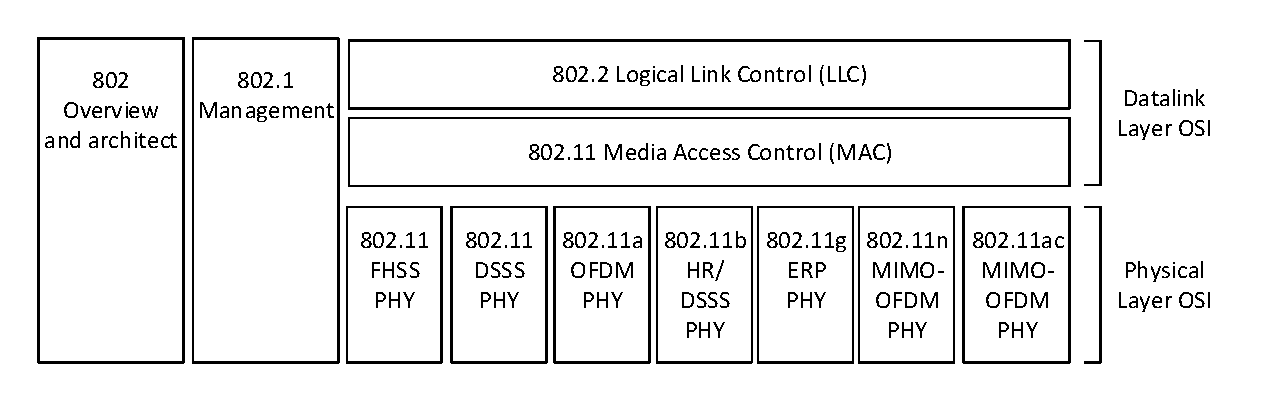
\includegraphics[width=1.0\textwidth]{80211-reference-osi}
    \caption{
        \label{fig:80211-reference-osi}
        Kiến trúc 802.11 và sự tham chiếu trong mô hình OSI}% ~\cite{gast2005802}
\end{figure}

Hình~\ref{fig:80211-reference-osi} cho thấy chuẩn 802.2 đặc tả lớp con điều khiển liên kết luận lý (LLC) chung, được sử dụng bởi các lớp bên dưới thuộc mọi công nghệ LAN, nhằm tạo tính tương thích giữa chúng cũng như cung cấp cái nhìn trong suốt từ các lớp bên trên (từ lớp ứng dụng cho tới lớp mạng). Bên cạnh đó, các mạng 802 đều có một lớp con điều khiển truy cập thiết bị (MAC) và lớp vật lý (PHY) riêng, trong đó:
\begin{itemize}
\item Lớp con điều khiển truy cập thiết bị (MAC) là một tập các luật xác định cách thức truy cập thiết bị phần cứng và gửi dữ liệu.
\item Lớp vật lý (PHY) đảm nhiệm chi tiết việc gửi và nhận dữ liệu bằng thiết bị phần cứng.
\end{itemize}

Các chuẩn thường gặp như 802.11a, 802.11b, 802.11g, 802.11n và gần đây là 802.11ac được dùng để đặc tả những yêu cầu kỹ thuật khác nhau ở lớp vật lý.

\subsection{Các mô hình mạng}

\subsubsection{Các thành phần chính}
Mạng WiFi gồm bốn thành phần vật lý chính, được tóm tắt như Hình~\ref{fig:80211-architecture}.

\begin{itemize}
\item \emph{Trạm (Station - STA):} các trạm tham gia truyền dữ liệu trong mạng thông qua card mạng không dây như máy tính xách tay, điện thoại thông minh.
\item \emph{Điểm truy cập (Access Point - AP):} là thiết bị trung gian, điều khiển kết nối không dây trong mạng WiFi cũng như giữa chúng với mạng có dây.

\begin{figure}[H]
    \centering
    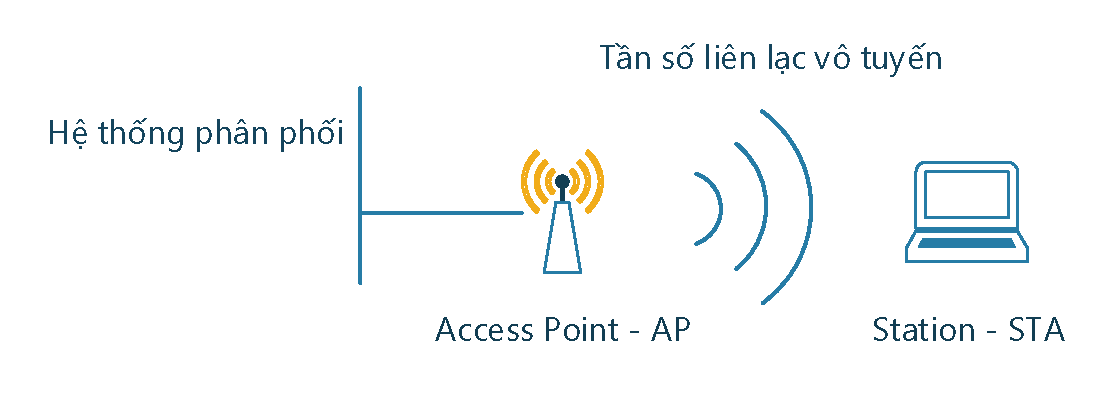
\includegraphics[width=1.0\textwidth]{80211-architecture}
    \caption{
        \label{fig:80211-architecture}
        Các thành phần vật lý của mạng WiFi}% ~\cite{gast2005802}
\end{figure}

\item \emph{Tần số liên lạc vô tuyến (Wireless Medium):} tùy theo đặc tả kỹ thuật của chuẩn cụ thể, cũng như loại sóng vô tuyến được sử dụng, các thiết bị sẽ cần một tần số liên lạc vô tuyến nhất định để truyền dữ liệu trong mạng WiFi.
\item \emph{Hệ thống phân phối (Distribution System):} bằng cách nối thêm các điểm truy cập, mạng WiFi có thể bao phủ một phạm vi lớn hơn.
\end{itemize}

\subsubsection{Các mô hình mạng}
Trong mạng WiFi có hai mô hình mạng phổ biến: mô hình mạng độc lập (Ad-hoc hay Independent BSS) và mô hình mạng cơ cở (Infrastructure BSS). Trong mô hình mạng độc lập, các STA tập trung lại trong một không gian nhỏ để hình thành nên kết nối ngang hàng giữa chúng.%~\cite{gast2005802}.

Các STA trong mô hình mạng cơ cở liên lạc với nhau thông qua AP. AP là điểm trung tâm quản lý mọi sự giao tiếp trong mạng. Để giao tiếp với nhau, các STA khác phải gửi các khung đến AP, sau đó AP sẽ gửi đến STA nhận. Một mô hình mạng cơ sở đơn giản với một AP được gọi là tập dịch vụ cơ bản (Basic Service Set - BSS). Một mạng có nhiều hơn một AP tạo thành một mạng gọi là tập dịch vụ mở rộng (Extended Service Set - ESS).%~\cite{gast2005802}.

Trong mô hình mạng cơ sở có hai khái niệm cơ bản là định danh tập dịch vụ (Service Set Identifier - SSID) và định danh tập dịch vụ cơ bản (Basic Service Set Identifier - BSSID). SSID là một định danh duy nhất gồm 32 ký tự chứa trong tiêu đề hoặc gói tin được gửi trên mạng hoạt động như một mật khẩu khi STA cố gắng thiết lập kết nối với BSS~\cite{vasseur2010interconnecting}. SSID phân biệt một mạng WiFi này với một mạng WiFi khác, vì vậy tất cả các AP và thiết bị cố gắng kết nối với một mạng WiFi cụ thể phải sử dụng cùng một SSID. SSID cũng được coi là tên mạng vì nó có thể dễ dàng đọc được. BSSID là một trường có độ dài 48 bit giống như địa chỉ MAC, trường này là định danh duy nhất cho mỗi BSS, giá trị của nó chính là địa chỉ MAC của AP~\cite{ieee2007802}.

\subsection{Khung quản lý}
\newcommand\tab[1][2.5mm]{\hspace*{#1}}
Chuẩn 802.11 định nghĩa một số loại khung (frame) khác nhau để các STA và AP sử dụng để liên lạc, cũng như quản lý và kiểm soát các liên kết không dây. Có ba loại khung chính, trong đó khung quản lý (management frame) cho phép các STA thiết lập và duy trì liên lạc. Dưới đây là một số loại phụ của khung quản lý~\cite{geier2001wireless}:
\begin{itemize}
\item \emph{Khung yêu cầu liên kết (association request):} \tab Một STA sẽ gửi khung này đến một AP nếu muốn liên kết với AP đó. Một STA sẽ được liên kết với một AP sau khi AP đó cho phép.

\item \emph{Khung đáp ứng liên kết (association response):} \tab Sau khi một AP nhận được một khung yêu cầu liên kết, AP sẽ gửi một khung đáp ứng liên kết để cho biết có chấp nhận sự liên kết với STA gửi hay không.

\item \emph{Khung yêu cầu liên kết lại (reassociation request):} \tab Một STA sẽ gửi khung này đến một AP nếu nó muốn liên kết lại với AP đó. Sự liên kết lại có thể xảy ra nếu một STA di chuyển ra ngoài phạm vi của một AP và trong phạm vi của một AP khác. STA sẽ cần liên kết với AP mới để AP mới biết rằng nó sẽ cần thương lượng chuyển tiếp các khung dữ liệu từ AP cũ.

\item \emph{Khung đáp ứng liên kết lại (reassociation response):} \tab Sau khi một AP nhận được một khung yêu cầu liên kết lại, AP sẽ gửi một khung đáp ứng liên kết lại để cho biết có chấp nhận việc liên kết lại với STA gửi không.

\item \emph{Khung yêu cầu thăm dò (probe request):} \tab Một STA gửi một khung yêu cầu thăm dò để thu thập thông tin từ một STA hoặc AP khác. Ví dụ, một STA có thể gửi một khung yêu cầu thăm dò để xác định có một AP nào đó hiện diện hay không.

\item \emph{Khung đáp ứng thăm dò (probe response):} \tab Nếu STA hoặc AP nhận được một khung yêu cầu thăm dò, nó sẽ trả lời STA gửi bằng một khung đáp ứng thăm dò có chứa các thông số cụ thể về chính nó (chẳng hạn như các tham số cho trải phổ nhảy tần và trải phổ trực tiếp ở lớp vật lý).

\item \emph{Khung báo hiệu (beacon):} \tab Trong mô hình mạng cơ sở, một AP định kỳ gửi một báo hiệu (theo tham số aBeaconPeriod trong MIB) cung cấp sự đồng bộ giữa các STA sử dụng lớp PHY giống nhau. Beacon bao gồm một dấu thời gian mà tất cả các STA sử dụng để cập nhật những gì 802.11 định nghĩa như một bộ đếm thời gian đồng bộ hóa chức năng (TSF). Nếu một AP hỗ trợ chức năng điều phối điểm, thì nó sử dụng một khung báo hiệu để thông báo sự bắt đầu của thời kỳ không tranh chấp. Nếu mạng có mô hình mạng độc lập (tức là nó không có AP), tất cả các STA định kỳ gửi báo hiệu cho mục đích đồng bộ hóa.

\item \emph{Khung thông báo chỉ dẫn lưu thông (Announcement Traffic Indication Message - ATIM):} \tab Một STA với khả năng lưu tạm các khung cho các STA khác, sẽ gửi một khung ATIM cho mỗi STA thông qua cửa sổ ATIM, ngay sau khi một thăm dò được truyền. Sau đó, STA truyền những khung này tới những STA nhận thích hợp. Việc truyền tải các khung ATIM cảnh báo cho các STA đang trong trạng thái ngủ, để chuyển sang trạng thái thức đủ lâu để nhận các khung tương ứng.

\item \emph{Khung hủy bỏ liên kết (disassociation):} \tab Nếu một STA hoặc AP muốn kết thúc một liên kết, nó sẽ gửi một khung hủy bỏ liên kết đến STA đối diện. Một khung hủy bỏ liên kết đơn có thể kết thúc các liên kết với nhiều hơn một STA thông qua địa chỉ quảng bá của tất cả chúng.

\item \emph{Khung xác thực (authentication):} \tab Một STA gửi một khung xác thực đến một STA hoặc AP mà nó muốn xác thực. Trình tự xác thực bao gồm việc truyền một hoặc nhiều khung xác thực, tùy thuộc vào loại xác thực được thực hiện (hệ thống mở hay khoá chia sẻ).

\item \emph{Khung hủy bỏ xác thực (deauthentication):} \tab Một STA gửi một khung hủy bỏ xác thực tới một STA hoặc AP mà nó muốn kết thúc các liên lạc an toàn.
\end{itemize}

SSID là một phần của một số khung quản lý. Các thông điệp quản lý luôn luôn được gửi dưới dạng rõ, thậm chí khi mã hóa liên kết (ví dụ như WEP) được sử dụng~\cite{gast2005802}, vì vậy ai cũng có thể có được SSID dễ dàng khi chặn bắt các khung này.

Ngoài khung quản lý, còn có khung điều khiển (control frame) và khung dữ liệu (data frame). Sau khi thiết lập liên kết và xác thực giữa STA và AP, khung điều khiển hỗ trợ việc phân phát các khung dữ liệu. Mục đích chính của các khung dữ liệu là mang các thông tin, tới STA đích để chuyển đến lớp LLC thích hợp của nó. Các khung dữ liệu này có thể mang thông tin cụ thể như địa chỉ MAC nguồn và đích, BSSID.

\subsection{Xác thực và liên kết}
Trong kết nối với AP, STA thực hiện nhiều giai đoạn, trong đó cần chú ý là xác thực (authentication) và liên kết (association). Cụ thể các giai đoạn có thể được nhìn thấy trong Hình~\ref{fig:authentication-and-association}. Tất cả các STA bắt đầu ở trạng thái 1, và chỉ có thể truyền dữ liệu đến một hệ thống phân phối khi ở trong trạng thái 3. Hình vẽ cũng cho thấy các khung được chia thành các lớp khác nhau. Khung lớp 1 có thể truyền trong trạng thái 1; các khung lớp 1 và 2 truyền trong trạng thái 2; và các khung lớp 1, 2, và 3 truyền trong trạng thái 3. Các khung phụ của khung quản lý được phân loại như Bảng~\ref{tab:management-class}~\cite{gast2005802}.

\begin{figure}[H]
    \centering
    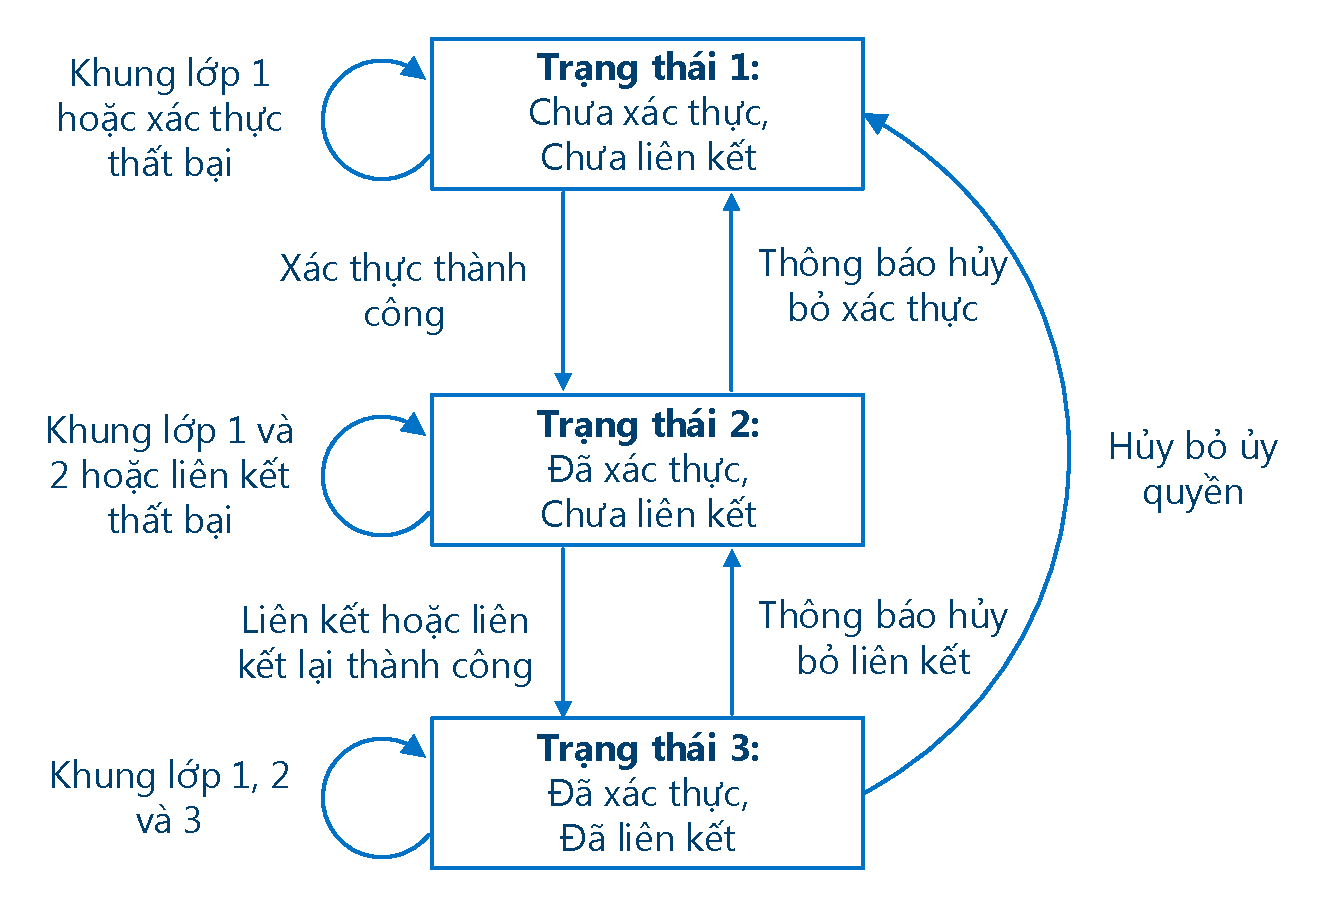
\includegraphics[width=1.0\textwidth]{authentication-and-association}
    \caption{
        \label{fig:authentication-and-association}
        Các giai đoạn xác thực và liên kết}% ~\cite{bidgoli2005hacking}
\end{figure}

\subsubsection*{\textit{a) Xác thực}}
\emph{Xác thực} là quá trình chứng minh nhận dạng của một STA đến STA khác hoặc AP. Trong xác thực hệ thống mở, tất cả các STA đều được xác thực mà không cần bất kỳ kiểm tra nào. Một STA A gửi một khung yêu cầu xác thực có chứa danh tính A, đến STA B. STA B trả lời với một khung cho biết sự công nhận, gửi tới A. Trong kiến trúc mạng khép kín, các STA phải biết SSID của AP để kết nối với AP. Xác thực khóa chia sẻ thì sử dụng một tiêu chuẩn thách đố và giải đố cùng với khóa bí mật chia sẻ. Trong phần sau, đồ án sẽ trình bày rõ hơn về một số tiêu chuẩn xác thực và mã hóa.

\begin{table}[!htbp]
\centering
\small
\setlength{\extrarowheight}{1pt}
\caption{\label{tab:management-class}Phân loại khung quản lý theo lớp}
\begin{tabular}{|c|p{10cm}|}
\hline
\textbf{Phân loại}     & \textbf{Tên khung}                            \\ \hline
\multirow{6}{*}{Lớp 1} & Probe Request                                 \\ \cline{2-2} 
                       & Probe Response                                \\ \cline{2-2} 
                       & Beacon                                        \\ \cline{2-2} 
                       & Authentication                                \\ \cline{2-2} 
                       & Deauthentication                              \\ \cline{2-2} 
                       & Announcement Traffic Indication Message (ATIM) \\ \hline
\multirow{3}{*}{Lớp 2} & Association Request/Response                  \\ \cline{2-2} 
                       & Reassociation Request/Response                \\ \cline{2-2} 
                       & Disassociation                                \\ \hline
Lớp 3                  & Deauthentication                              \\ \hline
\end{tabular}
\end{table}

\subsubsection*{\textit{b) Liên kết}}

Trao đổi dữ liệu giữa AP và STA chỉ có thể xảy ra khi STA đã được liên kết với AP trong mô hình mạng cơ sở hoặc với một STA khác ở mô hình mạng độc lập. Tất cả các AP truyền khung báo hiệu một số lần trong mỗi giây. Khung báo hiệu có chứa SSID, thời gian, khả năng, tốc độ và các thông tin khác. Liên kết có hai quá trình. Một STA mà chưa được xác thực và chưa liên kết sẽ lắng nghe khung báo hiệu để lựa chọn BSS mà nó muốn tham gia vào. STA và AP cùng nhau xác thực bằng cách trao đổi các khung xác thực. Khi đó, STA hiện đã được xác thực nhưng chưa được liên kết. Trong giai đoạn thứ hai, STA gửi khung yêu cầu liên kết và AP sẽ phản hồi lại một khung đáp ứng liên kết có chứa ID liên kết với STA. Khi đó, STA đã được xác thực và liên kết.

\subsection{Các tiêu chuẩn mã hóa}
Trong bảo mật mạng WiFi, người dùng thường chỉ quan tấm đến mật khẩu WiFi. Tuy nhiên cái thật sự quan trọng bên dưới chính là tiêu chuẩn mã hóa, việc lựa chọn tiêu chuẩn mã hóa phù hợp sẽ mang lại độ an toàn cao hơn cho mạng. Hầu hết các AP đều có khả năng cho phép một trong ba tiêu chuẩn mã hóa sau: Wired Equivalent Privacy (WEP), Wi-Fi Protected Access (WPA) hoặc Wi-Fi Protected Access II (WPA2).

Ngoài ra, chuẩn 802.11 cũng cho phép sử dụng hệ thống mở (Open System), tức là không sử dụng mã hóa các dữ liệu trong mạng. Tuy nhiên điều này tiềm ẩn nguy cơ về các vấn đề bảo mật, do vậy thường không được khuyến nghị sử dụng.

\subsubsection{WEP}
WEP là một giao thức mã hóa mặc định được giới thiệu lần đầu trong chuẩn IEEE 802.11 vào năm 1999. Nó sử dụng thuật toán mã dòng RC4 cho việc xác thực và mã hóa. Chuẩn này định nghĩa một khóa bí mật chia sẻ có độ dài 40 bit hoặc 104 bit. Khóa phải được quản trị viên nhập vào và cập nhật thủ công.

Khóa được kết hợp với một vector khởi tạo (IV) 24 bit nhằm mục đích tăng sức mạnh mã hóa. Tuy nhiên, kích thước IV nhỏ làm tăng khả năng khóa sẽ được sử dụng lại. Cùng với một số lỗ hỏng trong cơ chế xác thực, WEP ngày càng ít được sử dụng~\cite{guillaume2005wifi}.

\subsubsection{WPA}
Quá nhiều lỗ hỏng tồn tại trong WEP cho thấy nhu cầu cấp thiết cần một sự thay thế. Năm 2003, WiFi Alliance đã phát hành WPA như một tiêu chuẩn tạm thời, trong khi IEEE đang làm việc để phát triển một sự thay thế cao hơn, lâu dài hơn cho WEP. WPA có hai chế độ riêng cho người dùng doanh nghiệp và người dùng cá nhân. Chế độ doanh nghiệp, WPA-EAP, sử dụng xác thực 802.1x nghiêm ngặt hơn, với giao thức xác thực mở rộng EAP. Chế độ cá nhân, WPA-PSK, sử dụng các khóa được chia sẻ trước (pre-shared key) để thực hiện và quản lý đơn giản cho các khách hàng và văn phòng nhỏ. Chế độ doanh nghiệp yêu cầu sử dụng một máy chủ xác thực riêng~\cite{guillaume2005wifi}.

Mặc dù WPA cũng dựa trên thuật toán RC4, nhưng nó đã có một số cải tiến về mã hóa, cụ thể là việc sử dụng giao thức toàn vẹn khóa tạm thời (TKIP). Giao thức này bao gồm các tập chức năng để cải thiện bảo mật cho mạng WiFi: sử dụng khóa 256 bit, trộn khóa trên mỗi gói tin, tự động quảng bá các khóa được cập nhật, kiểm tra tính toàn vẹn thông điệp, kích thước IV lớn hơn (48 bit) và cơ chế giảm thiểu việc sử dụng lại IV.

WPA được thiết kế để tương thích ngược với WEP nhằm khuyến khích việc áp dụng nhanh chóng và dễ dàng. Chỉ với một bản cập nhật firmware mới, các thiết bị có thể hỗ trợ WPA với độ an toàn cao hơn.

\subsubsection{WPA2}
Tiêu chuẩn WPA2 hay còn gọi là 802.11i, được IEEE phê chuẩn vào năm 2004. Giống như WPA, WPA2 cũng cung cấp các chế độ dành cho doanh nghiệp và cá nhân. Mặc dù WPA2 còn tồn tại lỗ hỏng, nó vẫn được coi là chuẩn bảo mật mạng không dây an toàn nhất hiện có.

WPA2 thay thế thuật toán RC4 và TKIP bằng hai cơ chế mã hóa và xác thực mạnh hơn: chuẩn mã hóa nâng cao (AES) và giao thức CCMP. Ngoài ra để hỗ trợ tương thích ngược, WPA2 hỗ trợ TKIP như là một dự phòng nếu một thiết bị không thể hỗ trợ CCMP.

\subsection{Các tấn công trong mạng WiFi}
Phía sau sự tiện lợi của mạng WiFi, là khá nhiều mối đe dọa, đặc biệt là do các tấn công gây nên. Mục tiêu của chúng là những dữ liệu thông thường cho đến dữ liệu quan trọng, các tài khoản và dữ liệu bí mật khác~\cite{MEKHAZNIA2015172}.

\subsubsection{Giả mạo địa chỉ MAC}
Thuật ngữ "giả mạo địa chỉ MAC" trong ngữ cảnh này có nghĩa là kẻ tấn công thay đổi địa chỉ MAC mà nhà sản xuất gán vào card mạng thành địa chỉ khác. Việc giả mạo địa chỉ MAC khác với việc giả mạo địa chỉ IP, trong đó kẻ tấn công gửi dữ liệu từ một địa chỉ nguồn tùy ý và không mong đợi bất kỳ phản hồi nào đối với địa chỉ IP nguồn thật. Việc giả mạo địa chỉ MAC được mô tả chính xác hơn là giả mạo hoặc che dấu địa chỉ MAC vì kẻ tấn công không tạo ra dữ liệu với địa chỉ nguồn khác với địa chỉ của nó. Khi kẻ tấn công ghi đè địa chỉ MAC của mình, kẻ tấn công tiếp tục sử dụng card mạng không dây để truyền và nhận từ cùng một địa chỉ MAC nguồn~\cite{joshua2003detecting}. Tấn công này giúp kẻ tấn công vượt qua các cơ chế lọc địa chỉ MAC, một cơ chế xác thực thường được sử dụng ở các thiết bị AP.

\subsubsection{Tấn công từ chối dịch vụ}
\subsubsection*{\textit{a) Làm lụt khung xác thực/khung liên kết}}
Tấn công này cố áp đảo AP bằng các khung xác thực và khung liên kết. Để làm lụt các liên kết, kẻ tấn công sẽ giả mạo địa chỉ MAC của STA, sau đó liên tục cố liên kết với AP. Một trường hợp khác, kẻ tấn công sẽ thay thế địa chỉ MAC, giả mạo một lúc nhiều STA. Điều này làm cho bộ nhớ và khả năng xử lý của AP giảm, khiến AP từ chối STA ban đầu~\cite{scott2011known}.
	
\subsubsection*{\textit{b) Làm lụt khung hủy bỏ xác thực}}
Tấn công này hoạt động bằng cách khai thác điểm yếu cố hữu trong mạng không dây và thường được sử dụng như một phương pháp để bắt đầu tấn công giả mạo AP (Rogue Access Point - RAP). Kẻ tấn công gửi các khung hủy bỏ xác thực đến một STA đã kết nối với AP. STA nhận được khung hủy bỏ xác thực sẽ hủy bỏ liên kết với AP ngay khi có thể. Tấn công này hoạt động là vì các khung quản lý của AP không được mã hóa dẫn đến khung hủy bỏ xác thực được gửi đi tùy ý, bởi vậy rất dễ giả mạo. Tấn công này có thể tấn công trực tiếp lên AP, bằng cách gửi khung hủy bỏ xác thực đến địa chỉ MAC quảng bá với địa chỉ nguồn giả mạo là của AP~\cite{scott2011known}.

Các tấn công làm lụt có thể được phát hiện, vì một số lượng lớn khung hủy bỏ xác thực hoặc tương tự, sẽ tạo nên sự bất thường trong lưu lượng mạng.

\subsubsection{Man-in-the-middle}
Kẻ tấn công sử dụng tấn công Man-in-the-middle (MITM) để chặn bắt hoạt động trong mạng. Tấn công MITM bắt đầu với việc cấu hình một AP giả mạo (Rogue Access Point - RAP) để giả mạo AP gốc. Sau đó kẻ tấn công buộc STA kết nối với RAP bằng cách thực hiện tấn công từ chối dịch vụ lên AP gốc, hoặc bằng cách cung cấp tín hiệu mạnh hơn AP gốc. STA thường kết nối với AP có tín hiệu mạnh hơn. Để đánh lừa STA một cách chắc chắn, RAP thực hiện kết nối với các mạng khác để vẫn cung cấp kết nối Internet như bình thường. Nếu thành công, kẻ tấn công sẽ có thể có được quyền kiểm soát các kết nối mạng của STA. Với MITM, kẻ tấn công có thể giả mạo một trang web xác thực không dây để thu thập ID và mật khẩu; và thu thập các trang web, tên người dùng và mật khẩu được sử dụng trên các trang web. Tấn công này có thể được phát hiện đối với hệ thống mạng có ít AP, đối với hệ thống có nhiều AP đặt ở các vị trí xa nhau sẽ rất khó bảo vệ.

\subsubsection{Brute force WPS}
Thiết kế của Wi-Fi Protected Setup (WPS) có những nhược điểm cơ bản. Vì vậy, kẻ tấn công có thể lợi dụng những điểm yếu này để dò ra mã PIN chỉ trong vòng vài giờ.  Hình~\ref{fig:brute-force-wps-pin} là sơ đồ tấn công brute force mã PIN WPS~\cite{stefan2011brute}. Kẻ tấn công có thể nhận biết được liệu một phần của mã PIN là đúng hay không từ phản hồi của AP. Nếu kẻ tấn công nhận được thông báo EAP-NACK sau khi gửi M4, điều này có nghĩa là nửa đầu của mã PIN là chính xác. Nếu kẻ tấn công nhận được thông báo EAP-NACK sau khi gửi M6, điều đó có nghĩa là nửa cuối của mã PIN là chính xác. Mã PIN bao gồm 8 chữ số, do đó xác suất số PIN có giá trị là \(10^{8}\) hay là 100,000,000. Với phương thức tấn công này, số lần tấn công tối đa sẽ giảm xuống \(10^{4} + 10^{4}\), gấp 20,000 lần. Kể từ số thứ 8 của mã PIN, là tổng kiểm tra của các số từ 1 đến 7, do đó, cuộc tấn công sẽ giảm xuống \(10^{4} + 10^{3}\), là 11,000 lần.

\begin{figure}[H]
    \centering
    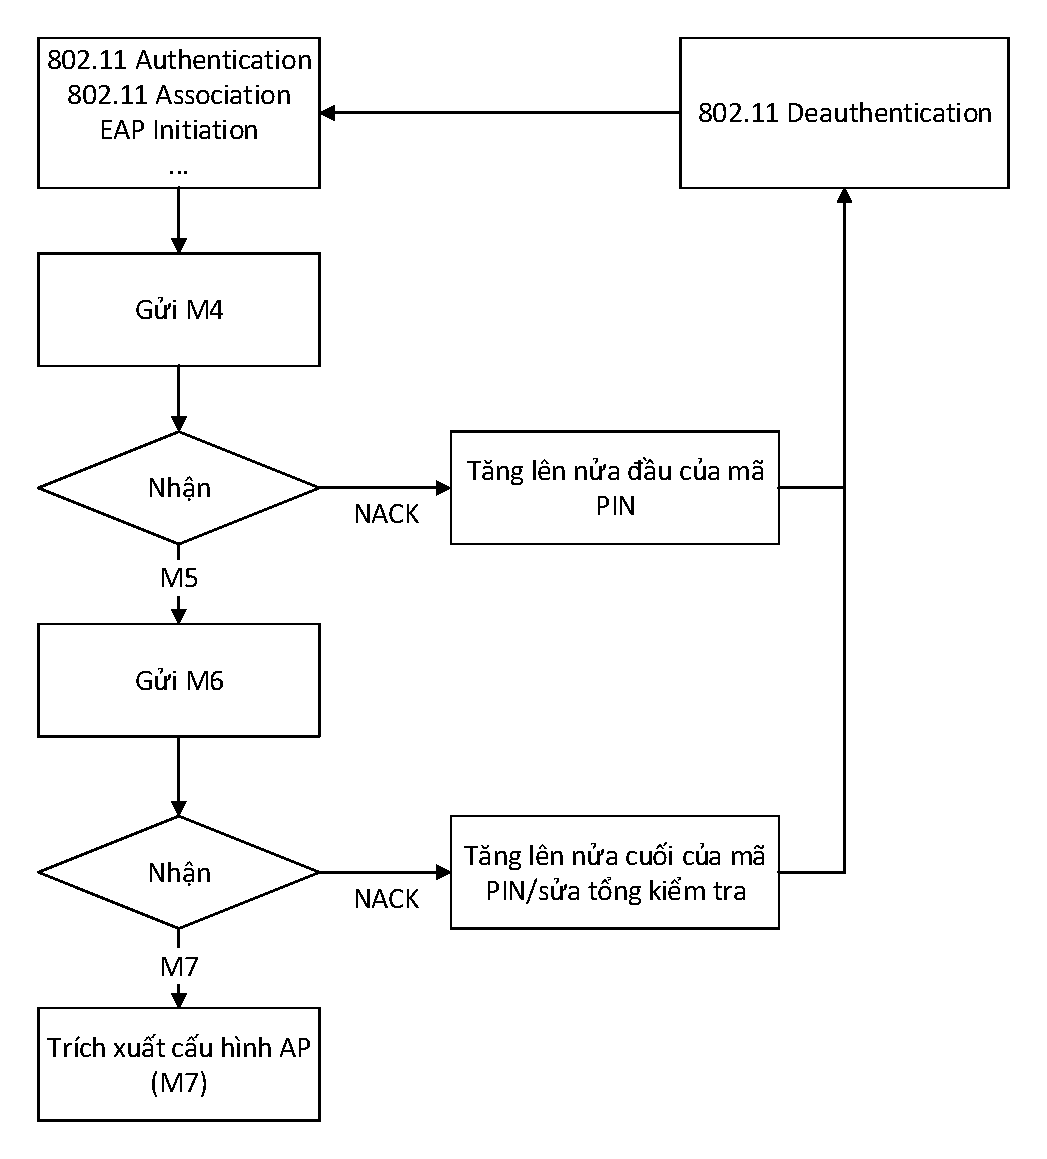
\includegraphics[width=0.85\textwidth]{brute-force-wps-pin}
    \caption{
        \label{fig:brute-force-wps-pin}
        Sơ đồ tấn công brute force mã PIN WPS}
\end{figure}

\begin{leftbar}
\noindent Ngoài những tấn công đặc trưng ở trên, người dùng trong mạng WiFi cũng có thể bị đe dọa bởi các tấn công tương tự như trong mạng có dây, như tấn công dò mật khẩu, tấn công quét cổng, phát tán mã độc, khai thác lỗ hỏng bảo mật. Trên đây là một số tấn công điển hình trong mạng WiFi, nhằm bảo vệ người dùng và phát hiện các mối đe dọa tiềm ẩn, mạng WiFi nên được thực hiện các giải pháp bảo mật, trong đó việc triển khai một hệ thống phát hiện xâm nhập là điều cần thiết.
\end{leftbar}

\section{Hệ thống phát hiện xâm nhập}
\subsection{Tổng quan}
\emph{Phát hiện xâm nhập} là quá trình giám sát các sự kiện xảy ra trong hệ thống máy tính hoặc mạng và phân tích các dấu hiệu của các sự cố có thể xảy ra, như là vi phạm hoặc đe dọa vi phạm chính sách bảo mật máy tính, các chính sách sử dụng được chấp nhận hoặc các tiêu chuẩn bảo mật trong thực tế. \emph{Ngăn chặn xâm nhập} là quá trình phát hiện xâm nhập và cố gắng ngăn chặn các sự cố có thể xảy ra. 

Theo tài liệu của Viện Tiêu chuẩn và Công nghệ Quốc gia Hoa Kỳ (NIST), hệ thống phát hiện xâm nhập (IDS) là các phần mềm tự động hóa quá trình phát hiện xâm nhập. Hệ thống ngăn chặn xâm nhập (IPS) là các phần mềm có tất cả chức năng của một hệ thống phát hiện xâm nhập và còn có thể cố gắng ngăn chặn các sự cố xảy ra nếu có thể~\cite{scarfone2007guide}. Như vậy, chức năng chính của IDS là tập trung vào việc xác định các sự cố có thể xảy ra, ghi lại thông tin về chúng, và báo cáo cho người quản trị. Trong phạm vi đồ án này, sẽ chỉ tập trung nghiên cứu về IDS, các chức năng chính và phương pháp phát hiện xâm nhập của nó.

\subsection{Các thành phần}
Các thành phần của một IDS bao gồm~\cite{scarfone2007guide}:

\begin{itemize}
\item \emph{Cảm biến và phần mềm đại diện (Sensor/Agent):} \tab Các cảm biến và phần mềm đại diện giám sát và phân tích các hoạt động. Các cảm biến thường được sử dụng để giám sát các mạng, và các phần mềm đại diện dùng để giám sát các máy tính đơn lẻ.

\item \emph{Máy chủ quản lý (Management Server):} \tab Một máy chủ quản lý là một thiết bị nhận các thông tin từ các cảm biến hoặc phần mềm đại diện và quản lý chúng. Nó cũng có thể thực hiện phân tích các thông tin nhận được và xác định các sự cố khi mà các cảm biến và phần mềm độc lập không thể.

\item \emph{Máy chủ cơ sở dữ liệu (Database Server):} \tab Một máy chủ cơ sở dữ liệu là một kho chứa cho các bản ghi thông tin sự kiện được ghi lại bởi các cảm biến, phần mềm đại diện, và các máy chủ quản lý.

\item \emph{Bảng điều khiển (Console):}  Một bảng điều khiển là một chương trình cung cấp một giao diện cho người sử dụng và quản trị viên của IDS. Bảng điều khiển thường được cài đặt lên các máy tính quản trị, phục vụ việc giám sát và quản trị IDS.
\end{itemize}

\subsection{Các chức năng chính}
Hiện nay có nhiều công nghệ IDS, được phân biệt chủ yếu bởi loại sự kiện mà chúng có thể nhận dạng và các phương pháp mà chúng sử dụng để xác định các sự cố. Ngoài chức năng chính là giám sát và phân tích các sự kiện để xác định các hoạt động không mong muốn. Hầu hết các công nghệ IDS đều có thể thực hiện các chức năng sau:

\begin{itemize}
\item \emph{Ghi lại các thông tin liên quan đến các sự kiện quan sát được:} \tab Thông tin có thể ghi lại cục bộ hoặc được gửi đến các hệ thống riêng biệt như máy chủ nhật ký tập trung, các giải pháp quản lý sự kiện an ninh (SIEM) và các hệ thống quản lý doanh nghiệp.

\item \emph{Thông báo cho các quản trị viên bảo mật về các sự kiện quan trọng được quan sát:} \tab Các thông báo này gọi chung là cảnh báo (alert). Chúng được gửi đến quản trị viên thông qua thư điện tử, thông điệp cảnh báo trên giao diện bảng điều khiển IDS, giao thức SMTP, thông điệp syslog và các chương trình và script do người dùng định nghĩa. Các thông báo này thường chỉ bao gồm thông tin cơ bản về sự kiện, quản trị viên cần truy cập IDS để biết thêm thông tin.

\item \emph{Xuất báo cáo:} \tab Báo cáo tóm tắt các sự kiện được theo dõi hoặc cung cấp chi tiết về các sự kiện cụ thể được quan tâm.
\end{itemize}

\subsection{Các phương pháp phát hiện phổ biến}
Các công nghệ IDS sử dụng nhiều phương pháp để phát hiện xâm nhập. Sau đây đồ án sẽ trình bày về các phương pháp phát hiện xâm nhập phổ biến bao gồm: \emph{phát hiện dựa trên chữ ký (signature-based)}, \emph{phát hiện dựa trên sự bất thường (anomaly-based)}, và \emph{phân tích giao thức có trạng thái (stateful protocol analysis)}~\cite{scarfone2007guide}. Hầu hết các sản phẩm IDS sử dụng nhiều phương pháp phát hiện, hoạt động độc lập hoặc kết hợp với nhau, để gia tăng phạm vi và độ chính xác cho việc phát hiện xâm nhập.

\subsubsection{Phát hiện dựa trên chữ ký}
\emph{Chữ ký} là một mẫu tương ứng với một mối đe dọa đã biết. \emph{Phát hiện dựa trên chữ ký} là quá trình so sánh các chữ ký với các sự kiện quan sát được để xác định các sự cố có thể xảy ra. Ưu điểm của phương pháp này là cho hiệu quả cao khi phát hiện các mối đe dọa đã biết. Tuy nhiên, nó không thể phát hiện các mối đe dọa chưa biết trước đó, các mối đe dọa sử dụng kỹ thuật lẩn trốn, và các biến thể của các mối đe dọa đã biết.

Phát hiện dựa trên chữ ký là một phương pháp phát hiện đơn giản nhất, vì nó chỉ thực hiện các hoạt động so sánh chuỗi. Các công nghệ phát hiện dựa trên chữ ký không có hiểu biết nhiều về các giao thức mạng hoặc ứng dụng, nên không thể theo dõi và hiểu được trạng thái của các liên lạc phức tạp. Chúng cũng thiếu khả năng ghi nhớ các yêu cầu trước đó khi xử lý yêu cầu hiện tại. Hạn chế này ngăn cản việc phát hiện các cuộc tấn công gồm nhiều sự kiện nhưng không có sự kiện nào có dấu hiệu rõ ràng về một cuộc tấn công.

\subsubsection{Phát hiện dựa trên sự bất thường}
\emph{Phát hiện dựa trên sự bất thường} là quá trình so sánh các định nghĩa về hoạt động được coi là bình thường với các sự kiện quan sát được để xác định độ lệch đáng kể. IDS sử dụng phương pháp phát hiện dựa trên sự bất thường có các hồ sơ biểu diễn các hành vi bình thường của người dùng, máy chủ, kết nối mạng hoặc ứng dụng. Các hồ sơ này được phát triển bằng cách giám sát các đặc tính của hoạt động điển hình trong một khoảng thời gian. Ví dụ, một hồ sơ cho một mạng cho thấy rằng hoạt động web trung bình chiếm 13\% băng thông mạng trong một ngày làm việc bình thường. IDS sau đó sử dụng các phương pháp thống kê để so sánh các đặc tính của hoạt động hiện tại với các ngưỡng có liên quan đến hồ sơ, chẳng hạn như phát hiện khi hoạt động web có băng thông cao hơn trung bình đáng kể và cảnh báo sự bất thường đến một quản trị viên. Các hồ sơ có thể được phát triển cho nhiều thuộc tính hành vi, chẳng hạn như số lượng thư điện tử được gửi bởi người dùng, số lần đăng nhập không thành công vào máy chủ và mức độ sử dụng bộ vi xử lý của máy chủ trong một khoảng thời gian nhất định.

Lợi ích chính của phương pháp phát hiện dựa trên sự bất thường là chúng rất hiệu quả khi phát hiện các mối đe dọa chưa biết trước đó. Một hồ sơ khởi tạo được sinh trong một khoảng thời gian định kỳ, còn được gọi là huấn luyện định kỳ. Hồ sơ cho phát hiện dựa trên sự bất thường có thể là hồ sơ tĩnh hoặc hồ sơ động. Hồ sơ tĩnh sau khi được sinh ra sẽ không thể thay đổi, trừ khi tạo thêm một hồ sơ mới. Hồ sơ động được điều chỉnh liên tục khi các sự kiện bổ sung được quan sát.

Phương pháp phát hiện dựa trên sự bất thường có nhược điểm là khả năng phát hiện dương tính giả cao. Ví dụ, các hoạt động bảo trì, sao lưu thường tạo ra lưu lượng truyền tải lớn, có thể bị cảnh báo như một hành vi bất thường.

\subsubsection{Phân tích giao thức có trạng thái}
\emph{Phân tích giao thức có trạng thái} là quá trình so sánh các hồ sơ đã xác định trước các sự kiện quan sát được để xác định độ lệch. Các hồ sơ này chứa các định nghĩa chung về hoạt động hợp lệ của giao thức được cho phép cho mỗi trạng thái của giao thức. Không giống như phát hiện dựa trên sự bất thường, sử dụng các hồ sơ máy chủ hoặc mạng cụ thể, phân tích giao thức có trạng thái dựa vào các hồ sơ chung được phát triển của nhà cung cấp để chỉ định cách mà các giao thức cụ thể nên và không nên sử dụng. Thuật ngữ "có trạng thái" trong phân tích giao thức có trạng thái có nghĩa là IDS có khả năng hiểu và theo dõi trạng thái của các giao thức ở lớp mạng, lớp vận chuyển và lớp ứng dụng mà có khái niệm về trạng thái.

Phân tích giao thức có trạng thái có thể xác định các câu lệnh có trình tự không mong muốn, chẳng hạn như các câu lệnh sử dụng lặp đi lặp lại hoặc sử dụng một câu lệnh mà không cần sử dụng câu lệnh ban đầu mà nó phụ thuộc. Một tính năng theo dõi trạng thái khác của phân tích giao thức có trạng thái là đối với các giao thức xác thực, IDS dựa vào đó để xác định các hoạt động khác nhau có thể chấp nhận đối với nhiều lớp người dùng hoặc người dùng cụ thể.

Phương pháp phân tích giao thức có trạng thái sử dụng các mô hình giao thức, thường dựa vào các tiêu chuẩn giao thức từ các nhà cung cấp phần mềm và các cơ quan phát hành tiêu chuẩn (ví dụ RFC của IETF). Nhiều tiêu chuẩn không giải thích đầy đủ chi tiết của giao thức, tạo nên những biến thể khi thực hiện giao thức. Ngoài ra, đối với các giao thức độc quyền, thông tin chi tiết về các giao thức thường không có sẵn, làm cho công nghệ IDS khó thực hiện phân tích chính xác và toàn diện.

Hạn chế chính của phương pháp phân tích giao thức có trạng thái là chúng cần rất nhiều tài nguyên do sự phức tạp của việc phân tích và chi phí liên quan trong việc thực hiện theo dõi trạng thái cho nhiều phiên đồng thời. Một vấn đề nghiêm trọng khác là các phương pháp phân tích giao thức có trạng thái không thể phát hiện các cuộc tấn công không vi phạm các đặc tính của các hành vi giao thức thông thường được chấp nhận, chẳng hạn như thực hiện nhiều hành động hợp lệ trong một khoảng thời gian ngắn để gây ra sự từ chối dịch vụ.

\subsection{Phân loại}
Hệ thống phát hiện xâm nhập có thể chia làm hai loại chính là hệ thống phát hiện xâm nhập mạng (NIDS) và hệ thống phát hiện xâm nhập máy chủ (HIDS). Mỗi loại có những chức năng và ưu nhược điểm riêng.

\subsubsection{Hệ thống phát hiện xâm nhập mạng}
\emph{Hệ thống phát hiện xâm nhập mạng} hoạt động như một thiết bị độc lập trên mạng. Nó thường được đặt ở các phân đoạn mạng hoặc các điểm kết nối giữa các vùng mạng khác nhau. Nhờ đó nó có thể giám sát lưu lượng mạng từ nhiều nguồn khác nhau trong vùng mạng đó. NIDS có thể là một thiết bị phần cứng hoặc phần mềm. Về cấu trúc thì NIDS thường bao gồm một tập hợp các cảm biến (sensor) được đặt ở các điểm khác nhau trong mạng. Các cảm biến này sẽ thực hiện giám sát lưu lượng mạng, thực hiện phân tích cục bộ lưu lượng mạng đó và báo cáo về cho trung tâm quản lý (Center Management Console). Snort, Suricata là những NIDS điển hình.

Ưu điểm của NIDS là có thể quản lý được cả một phân đoạn mạng gồm nhiều máy, với một mạng được thiết kế tốt, nó mang lại sự hiệu quả về mặt chi phí đáng kể. Vì khả năng hoạt động ở chế độ lắng nghe bị động, có thể cài đặt và bảo trì NIDS đơn giản, không ảnh hưởng tới mạng, cung cấp sự bảo vệ "trong suốt" đối với cả người dùng và kẻ tấn công.

Bên cạnh đó, NIDS có thể gặp những khó khăn trong việc xử lý tất cả các gói tin trong một mạng có kích thước lớn và mật độ lưu lượng cao, khả năng NIDS bị quá tải và không thể phát hiện được các tấn công là rất lớn. NIDS cũng biểu lộ nhược điểm khi làm việc với dữ liệu phân mảnh hay mã hóa, nó không thể phân tích được các thông tin đã bị mã hóa, và các dạng tấn công phân mảnh dữ liệu.

\subsubsection{Hệ thống phát hiện xâm nhập máy chủ}
\emph{Hệ thống phát hiện xâm nhập máy chủ} hoạt động trên một máy tính đơn lẻ. HIDS sẽ sử dụng các tài nguyên của máy chủ đó để theo dõi lưu lượng truy cập và phát hiện các cuộc tấn công nếu có. Bằng cách này HIDS có thể theo dõi được tất cả các hoạt động trên máy tính đó như tập tin nhật ký và những lưu lượng mạng ra vào nó. Ngoài ra HIDS còn theo dõi hệ điều hành, các sự kiện, các thông báo lỗi của máy chủ. Không phải hầu hết các cuộc tấn công đều thông qua mạng, nên không phải lúc nào NIDS cũng có thể phát hiện được cuộc tấn công trên một máy tính. Ví dụ, kẻ tấn công có quyền truy cập vật lý, từ đó có thể xâm nhập vào máy tính đó mà không cần tạo ra bất cứ lưu lượng mạng nào. Một ưu điểm của HIDS so với NIDS đó là nó có thể phát hiện các dạng tấn công phân mảnh dữ liệu. Bởi vậy nên HIDS thường được cài đặt trên các trên các máy chủ quan trọng của tổ chức, các máy chủ trong vùng DMZ. Một số HIDS phổ biến đó là OSSEC, Proventia Desktop.

Ngoài khả năng phát hiện các dạng tấn công phân mảnh dữ liệu, HIDS cũng có thể làm việc với dữ liệu mã hóa. Tuy nhiên, do phải cài đặt phần mềm giám sát (agent) lên các máy tính cần bảo vệ, nên nó đặt ra khá nhiều vấn đề cho công tác quản lý, cấu hình, cập nhật. HIDS cũng chiếm một phần tài nguyên hệ thống, và phụ thuộc nhiều vào hệ điều hành bên dưới nó, nên cần có những thiết lập tối ưu để mang lại hiệu quả phát hiện cao nhất.

\section{Hệ thống phát hiện xâm nhập mạng không dây}
\subsection{Giới thiệu}
Các hệ thống phát hiện xâm nhập được dùng để nhận diện mối đe dọa tới hệ thống mạng và máy tính bằng cách thu thập và phân tích dữ liệu. IDS thường chỉ được sử dụng cho hệ thống và mạng có dây. Trong thời gian gần đây, IDS đã được phát triển để sử dụng cho mạng không dây, được gọi là hệ thống phát hiện xâm nhập mạng không dây (Wireless Intrusion Detection System - WIDS). Những WIDS này có thể giám sát và phân tích hoạt động của người dùng và hệ thống, nhận biết các dạng tấn công đã biết, các hành vi bất thường trong mạng và các vi phạm chính sách cho mạng không dây. Các WIDS thu thập tất cả các liên lạc không dây cục bộ và tạo ra các cảnh báo dựa trên các chữ ký được xác định trước hoặc các bất thường trong lưu lượng truy cập.

WIDS cũng giống với một IDS chuẩn cho mạng có dây, nhưng thường yêu cầu về triển khai cũng như một số đặc tả chức năng riêng biệt để phát hiện xâm nhập cho mạng không dây.

\subsection{Các thành phần và kiến trúc}

\subsubsection{Các thành phần chính}
Các thành phần chính của WIDS giống với NIDS, bao gồm: bảng điều khiển, máy chủ cơ sở dữ liệu (tùy chọn), máy chủ quản lý, và cảm biến~\cite{scarfone2007guide}. Tất cả các thành phần (ngoại trừ các cảm biến) có chung chức năng cho tất cả các loại IDS. Cảm biến không dây thực hiện vai trò cơ bản giống như đối với cảm biến NIDS, nhưng chức năng rất khác bởi vì có nhiều phức tạp trong việc giám sát liên lạc không dây. Một cảm biến không dây chỉ có thể giám sát một kênh riêng lẻ tại một thời điểm, do đó có thể bỏ lỡ những hành vi trái phép trên các kênh khác. Vì vậy cảm biến sẽ thay đổi kênh thường xuyên, kỹ thuật này gọi là quét kênh (channel scanning), để có thể giám sát mỗi kênh một số lần trong mỗi giây.

Cảm biến không dây thông thường có một số dạng:
\begin{itemize}
\item \emph{Cảm biến riêng:} \tab Một cảm biến riêng là một thiết bị thực hiện các chức năng WIDS nhưng sẽ không hỗ trợ truyền dữ liệu từ nguồn tới đích. Nó sẽ hoạt động hoàn toàn bị động, một số chúng thực hiện phân tích lưu lượng, một số khác thì chuyển tiếp lưu lượng đến máy chủ quản lý để phân tích. Cảm biến riêng có thể được triển khai cố định tại các vị trí cụ thể hoặc di động.

\item \emph{Cảm biến đi kèm với một AP:} \tab Cảm biến đi kèm thường có khả năng phát hiện ít nghiêm ngặt như một cảm biến riêng vì AP cần phân chia thời gian giữa việc cung cấp truy cập mạng và giám sát trên nhiều kênh để phát hiện hành vi trái phép. Cảm biến này phù hợp cho việc giám sát ở một dải tần và kênh đơn lẻ.

\item \emph{Cảm biến đi kèm với một bộ chuyển mạch không dây:} \tab Bộ chuyển mạch không dây được dùng để quản lý và giám sát các thiết bị không dây. Tuy nhiên nó không cung cấp khả năng phát hiện mạnh như cảm biến đi kèm AP và cảm biến riêng.
\end{itemize}

\subsubsection{Kiến trúc mạng}
Các thành phần WIDS thường được kết nối với nhau thông qua mạng có dây, thể hiện giống như Hình~\ref{fig:wids-architecture}. Một mạng quản lý tách biệt hoặc mạng chuẩn của tổ chức có thể sử dụng cho các liên lạc giữa các thành phần của WIDS.

\begin{figure}[!h]
    \centering
    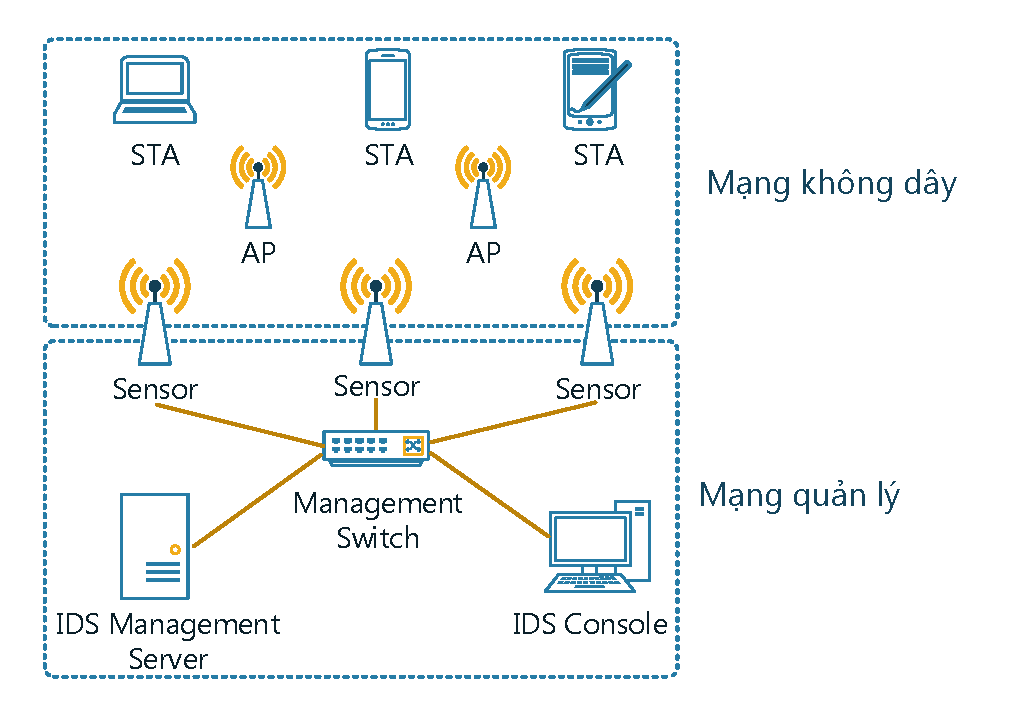
\includegraphics[width=1.0\textwidth]{wids-architecture}
    \caption{
        \label{fig:wids-architecture}
        Kiến trúc chung của WIDS}
\end{figure}

\subsection{Các tính năng bảo mật}

\subsubsection{Thu thập thông tin}
Hầu hết WIDS có thể thu thập các thông tin trên thiết bị không dây. Điển hình là nhận dạng các thiết bị trong mạng, bao gồm các AP, các STA, dựa trên BSSID và địa chỉ MAC của card mạng không dây. Ngoài ra, hầu hết các cảm biến cũng theo dõi các mạng, đánh dấu mạng nào được ủy quyền, mạng nào là mạng bên ngoài tổ chức hoặc các mạng giả mạo.

\subsubsection{Ghi nhật ký}
Các WIDS thường thực hiện mở rộng việc ghi nhật ký dữ liệu liên quan để phát hiện các sự kiện an ninh. Những dữ liệu này có thể được sử dụng để xác nhận tính hợp lệ của các cảnh báo, để điều tra các sự cố, và các mối liên hệ giữa IDS và các nguồn nhật ký khác. Các loại dữ liệu thường được ghi nhật ký bởi WIDS bao gồm:

\begin{itemize}
\item Nhãn thời gian
\item Loại sự kiện hoặc cảnh báo
\item Mức độ ưu tiên hoặc nghiêm trọng
\item Địa chỉ MAC nguồn (nhà sản xuất nào sẽ được nhận dạng)
\item Số thứ tự kênh
\item ID của cảm biến mà quan sát sự kiện
\item Hành động ngăn chặn đã thực hiện (nếu có tính năng ngăn chặn xâm nhập)
\end{itemize}

\subsubsection{Phát hiện xâm nhập}
Cũng giống như một hệ thống phát hiện xâm nhập thông thường, WIDS có thể phát hiện các tấn công, cấu hình sai, và vi phạm chính sách ở mức giao thức mạng không dây. WIDS thường không kiểm tra các truyền thông ở các mức cao (ví dụ như địa chỉ IP, dữ liệu lớp ứng dụng). Một số sản phẩm thực hiện chỉ kỹ thuật phát hiện dựa trên chữ ký, trong khi số khác sử dụng kết hợp các kỹ thuật phát hiện dựa trên chữ ký, phát hiện dựa trên hành vi bất thường, và phân tích giao thức có trạng thái. Dưới đây là các loại sự kiện thường được phát hiện bởi cảm biến WIDS~\cite{scarfone2007guide}:

\begin{itemize}
\item \emph{Mạng không dây hoặc thiết bị không dây trái phép:} \tab Thông qua khả năng thu thập thông tin, hầu hết các cảm biến WIDS có thể phát hiện các AP giả mạo, các STA trái phép, và cả các mạng trái phép.

\item \emph{Các thiết bị kém an toàn:} \tab Các WIDS có thể phát hiện các cấu hình sai, cũng như sử dụng các giao thức yếu. Điều này được thực hiện bằng cách xác định những sai khác từ các chính sách cụ thể của tổ chức cho các cài đặt mã hóa, xác thực, SSID và kênh.

\item \emph{Mẫu hành vi sử dụng bất thường:} \tab Một số cảm biến có thể sử dụng phương pháp phát hiện dựa trên hành vi bất thường để phát hiện các mẫu sử dụng bất thường. Những mẫu sử dụng bất thường điển hình là những nỗ lực tham gia vào mạng thất bại trong một khoảng thời gian, hoặc các hoạt động mạng ngoài giờ.

\item \emph{Sử dụng các công cụ quét mạng:} \tab Các công cụ quét mạng được sử dụng để nhận dạng các điểm yếu và mất an toàn của mạng không dây. WIDS chỉ có thể phát hiện việc sử dụng các công cụ quét chủ động, tức chúng có phát sinh lưu lượng mạng. Chúng không thể phát hiện việc sử dụng các cảm biến mà đơn giản chỉ giám sát và phân tích lưu lượng quan sát được.

\item \emph{Các điều kiện và tấn công từ chối dịch vụ:} \tab Tấn công từ chối dịch vụ có thể được phát hiện thông qua phương pháp phân tích trạng thái giao thức hoặc hành vi bất thường. Các tấn công từ chối dịch vụ được phát hiện thường được theo dõi trong suốt một thời gian và cảnh báo khi mà đạt đến một giá trị ngưỡng.

\item \emph{Các tấn công giả mạo và Man-in-the-middle:} \tab Một vài cảm biến WIDS có thể phát hiện khi mà một thiết bị cố gắng để giả mạo danh tính của thiết bị khác.
\end{itemize}

Hầu hết WIDS có thể xác định vị trí vật lý của một mối đe dọa được phát hiện bằng cách tính toán ước lượng khoảng cách gần đúng.

Mặc dù WIDS cung cấp khả năng phát hiện mạnh mẽ những chúng có một số hạn chế đáng kể. Một số vấn đề quan trọng như là không thể phát hiện được một số cuộc tấn công không dây, dễ bị trộm cắp, và không thể chịu được các cuộc tấn công chống lại chính WIDS. Cụ thể là tấn công không dây như giám sát bị động thì WIDS không thể phát hiện được. Thêm nữa, một cảm biến WIDS cũng dễ dàng bị tấn công, điển hình là tấn công từ chối dịch vụ sẽ làm gián đoạn chức năng của cảm biến.

\subsubsection{Khả năng quản lý}
Hầu hết sản phẩm WIDS có khả năng quản lý đơn giản. Sau khi lựa chọn sản phẩm WIDS, quản trị viên cần thiết kế một kiến trúc mạng, thực hiện kiểm tra các thành phần, đảm bảo an ninh cho các thành phần, và sau đó triển khai chúng. Vận hành và bảo trì WIDS gần giống như đối với NIDS. Bảng điều khiển WIDS cung cấp tính năng như quản lý, giám sát, phân tích, và báo cáo. Việc triển khai các WIDS có thể yêu cầu phải ngừng hoạt động mạng không dây trong một thời gian ngắn để nâng cấp hoặc cài đặt phần mềm IDS.

\section{Các hệ thống đã được phát triển}
Trong phần này, đồ án sẽ khảo sát về một số hệ thống WIDS đã được phát triển, bao gồm các sản phẩm WIDS từ các hãng nổi tiếng như Cisco, Netscout và một số dự án WIDS mã nguồn mở điển hình.

\subsection{Cisco Unified Wireless Network}
Cisco Unified Wireless Network (CUWN) là một giải pháp của Cisco giành cho doanh nghiệp. Nó cung cấp sự an toàn, khả năng mở rộng, và tiết kiệm chi phí cho mạng không dây doanh nghiệp~\cite{cisco2015enterprise}. CUWN gồm các thành phần chính là Aironet access points (AP), Wireless LAN controller (WLC), Cisco Prime Infrastructure và Mobility Services Engine (MSE); trong đó, WLC đóng vai trò là một thành phần phát hiện xâm nhập cho các tấn công trong mạng không dây. WLC thực hiện phân tích lưu lượng không dây của các AP đã kết nối và báo cáo khi phát hiện tấn công đến các WLC khác hoặc Wireless Control System (WCS). Ngoài ra, WLC cũng thực hiện phân tích bổ sung lưu lượng mạng có dây như một NIDS. Các tập tin chữ ký của WLC được bao gồm trong các bản phát hành phần mềm, nó cũng cho phép cập nhật độc lập từng tập tin, hoặc tự định nghĩa các chữ ký mới. Bảng dưới đây (Bảng~\ref{tab:cisco-wlc-signature}) là danh sách các chữ ký chuẩn của Cisco WLC~\cite{cisco2015enterprise}.

\begin{table}[h!]
\centering
\small
\setlength{\extrarowheight}{1pt}
\caption{\label{tab:cisco-wlc-signature}Các chữ ký chuẩn của Cisco WLC}
\begin{tabular}{|c|p{3.9cm}|c|p{6.8cm}|}
\hline
\multicolumn{1}{|l|}{\textbf{STT}} & \textbf{Tên}          & \textbf{Kiểu khung} & \textbf{Mô tả}                                 \\ \hline
1                                  & Bcast deauth          & Management          & Broadcast Deauthentication Frame               \\ \hline
2                                  & NULL probe resp 1     & Management          & NULL Probe Response - Zero length SSID element \\ \hline
3                                  & NULL probe resp 2     & Management          & NULL Probe Response - No SSID element          \\ \hline
4                                  & Assoc flood           & Management          & Association Request flood                      \\ \hline
5                                  & Auth flood            & Management          & Authentication Request flood                   \\ \hline
6                                  & Reassoc flood         & Management          & Reassociation Request flood                    \\ \hline
7                                  & Broadcast Probe flood & Management          & Broadcast Probe Request flood                  \\ \hline
8                                  & Disassoc flood        & Management          & Disassociation flood                           \\ \hline
9                                  & Deauth flood          & Management          & Deauthentication flood                         \\ \hline
10                                 & Reserved mgmt 7       & Management          & Reserved management sub-type 7                 \\ \hline
11                                 & Reserved mgmt F       & Management          & Reserved management sub-type F                 \\ \hline
12                                 & EAPOL flood           & Data                & EAPOL Flood Attack                             \\ \hline
13                                 & NetStumbler 3.2.0     & Data                & NetStumbler 3.2.0                              \\ \hline
14                                 & NetStumbler 3.2.3     & Data                & NetStumbler 3.2.3                              \\ \hline
15                                 & NetStumbler 3.3.0     & Data                & NetStumbler 3.3.0                              \\ \hline
16                                 & NetStumbler generic   & Data                & NetStumbler                                    \\ \hline
17                                 & Wellenreiter          & Management          & Wellenreiter                                   \\ \hline
\end{tabular}
\end{table}

Hơn thế, CUWN cũng cung cấp thành phần tích hợp Adaptive Wireless Intrusion Prevention System (wIPS) với khả năng ngăn chặn các cuộc tấn công trong mạng không dây. CUWN có thể gửi cảnh báo qua SNMP tới hệ thống quản lý WCS, và gửi thư điện tử qua SMTP đến nhà quản trị.

Tuy nhiên, so với thị trường như nước ta thì giá thành của giải pháp CUWN vẫn khá cao. Qua khảo sát, có thể thấy được chi phí để triển khai một giải pháp CUWN cơ bản của Cisco khoảng trên 8000 USD, bao gồm 1 Cisco Wireless Controler hỗ trợ cho 12 Access Point với giá 4000 USD~\cite{router2017airwlc}, 2 Access Point giá 1000 USD~\cite{router2017airap} cho hệ thống chỉ hỗ trợ 5 Access Point. Ngoài ra hệ thống này cũng cần có nhân viên quản trị được đào tạo để cài đặt, cấu hình, quản lý. Vì vậy, Cisco cũng cung cấp các khóa học để đào tạo và tổ chức thi các chứng chỉ quản trị cho hệ thống này.

\subsection{AirMagnet Enterprise}

Bên cạnh CUWN của Cisco, hãng bảo mật Netscout cũng đưa ra một giải pháp WIDS/IPS có tên là AirMagnet Enterprise. Kiến trúc của WIDS/IPS này gồm một hoặc nhiều máy chủ quản lý, được gọi là AirMagnet Enterprise Server (AME), và nhiều cảm biến WIDS/IPS, được gọi là AirMagnet Sensors và AirMagnet Spectrum Sensors. Hình~\ref{fig:ame-architect} mô tả kiến trúc của một hệ thống AirMagnet Enterprise điển hình.

\begin{figure}[H]
    \centering
    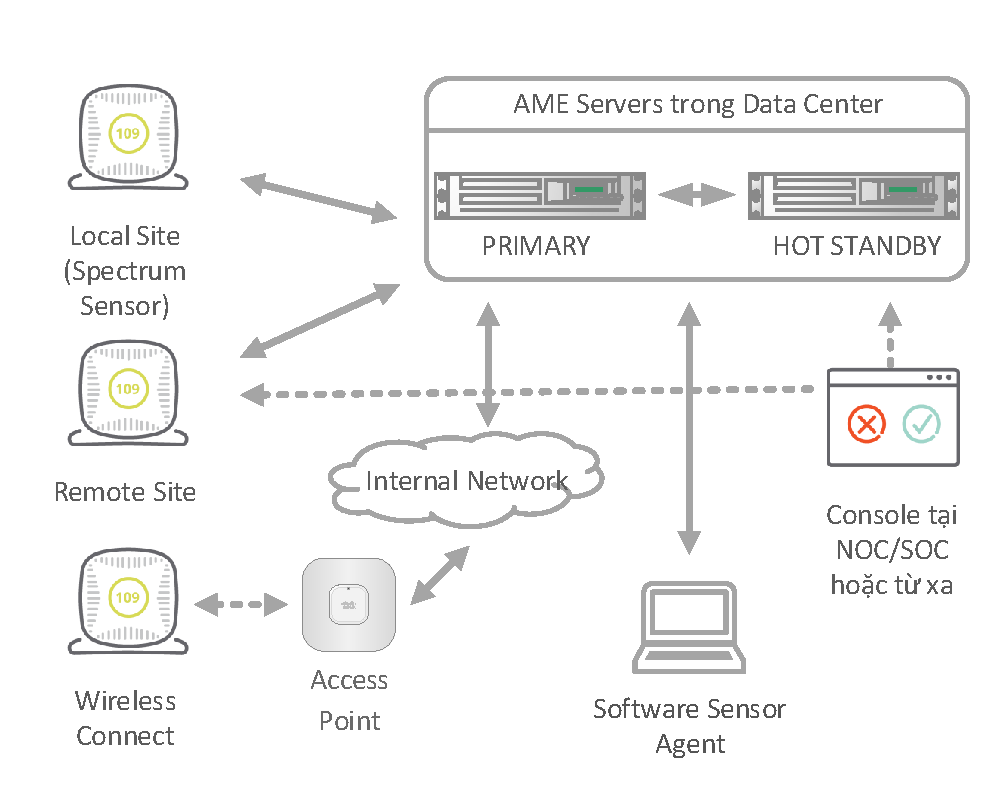
\includegraphics[width=0.8\textwidth]{ame-architect}
    \caption{
        \label{fig:ame-architect}
        Kiến trúc của AirMagnet Enterprise}
\end{figure}

Hầu hết WIDS/IPS đều có khả năng phát hiện tấn công mạng không dây cơ bản nhất như phát hiện ra AP giả mạo và các thiết bị STA trái phép. AirMagnet Enterprise không phải là ngoại lệ. Nó cũng cung cấp nhiều khả năng phát hiện tấn công tiên tiến, bao gồm phát hiện các tấn công từ chối dịch vụ và các tấn công giả mạo, cũng như lập bản đồ vị trí vật lý của các thiết bị STA và AP. AirMagnet Enterprise không cung cấp khả năng phát hiện tấn công xác thực và nỗ lực phá mã, đây là tính năng mà khá ít hệ thống WIDS/IPS hỗ trợ~\cite{karen2016fluke}.

Ưu điểm đáng lưu ý của AirMagnet Enterprise là cung cấp khả năng thu thập dữ liệu và báo cáo rất mạnh mẽ, nó có thể ghi lại tất cả các sự kiện cơ bản và thu thập các gói dữ liệu. Nó cũng hỗ trợ báo cáo theo các tiêu chuẩn tuân thủ bảo mật như PCI-DSS, HIPAA~\cite{karen2016fluke}.

\begin{leftbar}
\noindent Qua khảo sát hai sản phẩm khá nổi tiếng ở trên, có thể thấy chúng đều có khả năng giám sát và phát hiện các cuộc tấn công trong mạng không dây, lưu trữ các thông tin liên quan đến cuộc tấn công vào cơ sở dữ liệu, gửi cảnh báo qua SNMP, SMTP. Tuy nhiên, các giải pháp này đều chủ yếu giành cho đối tượng khách hàng doanh nghiệp với giá thành khá cao, thị trường doanh nghiệp nhỏ, trường học, hay quán cà phê vẫn đang bỏ ngỏ. Trong các phần dưới dây, đồ án sẽ trình bày về một số WIDS nguồn mở, điển hình là Snort Wireless và Kismet Wireless.
\end{leftbar}

\subsection{Snort Wireless}
Snort là một NIDS đã quá phổ biến. Vì vậy vào năm 2004, cộng đồng mã nguồn mở đã phát triển một dự án gọi là Snort Wireless, nhằm mở rộng khả năng của Snort để phát hiện các tấn công trong mạng không dây. Nó hoàn toàn tương thích ngược với Snort 2.0.x và thêm một số tính năng bổ sung. Snort Wireless đặc tả các luật thông qua một quy tắc luật mới, gọi là giao thức \emph{wifi}, có thể phát hiện hầu hết các tấn công trong mạng không dây như tấn công giả mạo, các công cụ quét mạng như Netstumbler~\cite{caswell2005nessus}. Bảng~\ref{tab:snort-wireless-rule-options} là danh sách các tùy chọn trong luật của Snort Wireless~\cite{valli2004wireless} .

\newgeometry{a4paper,left=3.5cm,right=2cm,top=3cm,bottom=3cm}
\headsep=0pt

\begin{table}[H]
\centering
\small
\setlength{\extrarowheight}{1pt}
\caption{\label{tab:snort-wireless-rule-options}Các tùy chọn trong luật của Snort Wireless}
\begin{tabular}{|p{4cm}|p{10.5cm}|}
\hline
\textbf{Tùy chọn} & \textbf{Mô tả}                                          \\ \hline
frame\_control    & kiểm tra trường điều khiển toàn bộ khung                \\ \hline
type              & kiểm tra kiểu khung của 802.11                          \\ \hline
stype             & kiểm tra kiểu khung phụ của 802.11                      \\ \hline
from\_ds          & kiểm tra cờ điều khiển khung từ hệ thống phân phối      \\ \hline
to\_ds            & kiểm tra cờ điều khiển khung đến hệ thống phân phối     \\ \hline
more\_frags       & kiểm tra cờ điều khiển trong các khung \emph{more fragment}    \\ \hline
retry             & kiểm tra cờ điều khiển trong khung \emph{retry}                \\ \hline
pwr\_mgmt         & kiểm tra cờ điều khiển trong các khung \emph{power management} \\ \hline
more\_data        & kiểm tra cờ điều khiển trong khung dữ liệu              \\ \hline
wep               & kiểm tra cờ điều khiển trong khung \emph{wep}                  \\ \hline
order             & kiểm tra cờ điều khiển thứ tự khung                      \\ \hline
duration\_id      & kiểm tra các trường \emph{duration-id} của khung                     \\ \hline
bssid             & kiểm tra trường BSSID của khung                                 \\ \hline
seqnum            & kiểm tra trường \emph{sequence number} của khung                \\ \hline
fragnum           & kiểm tra trường \emph{fragment number} của khung      \\ \hline
addr4             & kiểm tra trường địa chỉ thứ tư  của khung           \\ \hline
ssid              & kiểm tra trường SSID của khung                    \\ \hline
\end{tabular}
\end{table}

Luật của Snort Wireless có cú pháp như sau:

\begin{lstlisting}
<action> wifi <src mac> -> <dst mac> (<rule options>)
\end{lstlisting}

Cụ thể hơn, gói cài đặt Snort Wireless cũng cung cấp một số luật mặc định trong tập tin \emph{rules/wifi.rules}~\cite{caswell2005nessus}:\\

\begin{lstlisting}
alert wifi any -> any (msg:"Association Request"; stype:STYPE_ASSOCREQ;)
alert wifi any -> any (msg:"Association Response";stype:STYPE_ASSOCRESP;)
alert wifi any -> any (msg:"Reassociation Request"; stype:STYPE_REASSOC_ REQ;)
alert wifi any -> any (msg:"Reassociation Response"; stype:STYPE_REASSO C_RESP;)
alert wifi any -> any (msg:"Probe Request"; stype:STYPE_PROBEREQ;)
alert wifi any -> any (msg:"Probe Response"; stype:STYPE_PROBERESP;)
alert wifi any -> any (msg:"Beacon"; stype:STYPE_BEACON;)
\end{lstlisting}

\restoregeometry
\newgeometry{a4paper,left=3.5cm,right=2cm,top=3cm,bottom=3cm}
\headsep=0pt

\begin{lstlisting}
alert wifi any -> any (msg:"ATIM"; stype:STYPE_ATIM;)
alert wifi any -> any (msg:"Disassociation"; stype:STYPE_DISASSOC;)
alert wifi any -> any (msg:"Authentication"; stype:STYPE_AUTH;)
alert wifi any -> any (msg:"Deauthentication"; stype:STYPE_DEAUTH;)
\end{lstlisting}

Snort Wireless thực sự là một dự án WIDS tiềm năng, tuy nhiên hiện nay nó đã không còn được phát triển, dù chưa có thông báo chính thức nào. Các mã nguồn cài đặt và thư viện liên quan đều đã lỗi thời. Vì lý do này, trong hệ thống WIDS sẽ đề xuất, đồ án sẽ không lựa chọn Snort Wireless.

\subsection{Quadrant Information Security}
Quadrant Information Security cũng đưa ra một giải pháp WIDS miễn phí dựa trên các phần mềm mã nguồn mở~\cite{champ2014building}. Hệ thống này sử dụng một máy tính gồm một card mạng có dây và hai card mạng không dây. Card mạng có dây được kết nối ra Internet và chuyển tiếp các lưu lượng của AP ra Internet, card mạng không dây thứ nhất được dùng để giả lập AP thông qua phần mềm \emph{hostapd}, card mạng không dây còn lại đóng vai trò như một cảm biến WIDS để giám sát các tấn công lớp 2 từ bên ngoài mạng vào AP được giả lập. Snort được cài đặt như một NIDS, có thể giám sát lưu lượng không dây của AP. Kismet đảm nhiệm vai trò WIDS với cài đặt theo kiến trúc tiêu chuẩn, cả thành phần Kismet drone và Kismet server trên cùng máy tính. Như vậy, có thể thấy hệ thống WIDS này rất đa năng, có thể phát hiện được các tấn công bên trong và bên ngoài mạng không dây.

Đây là một thử nghiệm tuyệt vời về ưu điểm của các phần mềm mã nguồn mở, mang lại một giải pháp có giá thành thấp hơn rất nhiều so với các sản phẩm của các hãng như Cisco, Netscout. Tuy nhiên, nó cũng có nhược điểm lớn về triển khai, đó là kích thước của máy tính lớn hơn nhiều so với một AP, nên không thể đặt ở những vị trí treo tường hay ngoài trời, những nơi thực sự cần đặt cảm biến không dây. Hơn nữa, điện năng tiêu thụ và chi phí bảo trì phần cứng cũng cần được quan tâm, bởi vì một máy tính thông thường sẽ không phù hợp cho việc chạy liên tục trong một thời gian dài.

\restoregeometry

\section{Kismet Wireless}
\subsection{Giới thiệu}
Kismet là một ứng dụng phân tích mạng mã nguồn mở. Nó xác định các mạng bằng cách thụ động thu thập các gói tin. Kismet có thể phát hiện  các SSID ẩn và các mạng không quảng bá thông qua lưu lượng dữ liệu. Kismet có thể chạy với bất kỳ card mạng không dây nào hỗ trợ chế độ giám sát, và có thể chặn bắt lưu lượng 802.11b, 802.11a, 802.11g, và 802.11n. Ngoài ra, Kismet cũng có kiến trúc mở rộng, cho phép thêm các giao thức ngoài 802.11 để giải mã được~\cite{mike2016kismet}.

Các phần mở rộng của Kismet có thể thực hiện hầu hết mọi thứ giống như tiến trình Kismet có thể thực hiện. Phần mở rộng cho phép mở rộng khả năng ghi nhật ký, thêm các cảnh báo IDS, định nghĩa các nguồn thu mới và thêm các tính năng mới vào Kismet UI.

Kismet cung cấp tính năng WIDS cả có trạng thái và phi trạng thái cho các tấn công lên lớp 2 và lớp 3 của mạng không dây. Hiện tại tính năng phát hiện xâm nhập cho lớp 3 vẫn đang được phát triển. Kismet phát hiện tấn công và tạo cảnh báo dựa trên chữ ký - \emph{fingerprint} (cho các các tấn công đơn lẻ cụ thể) và dựa trên xu hướng/phân tích trạng thái - \emph{trend/stateful} (cho các tấn công sử dụng khung thăm dò bất thường, tấn công làm lụt khung hủy bỏ liên kết).

Kismet có thể tích hợp với các công cụ khác sử dụng \emph{tun/tap export} để cung cập một giao diện mạng ảo của lưu lượng không dây; các công cụ như Packet-o-Matic và Snort có thể sử dụng những dữ liệu đã xuất này để thực hiện các chức năng IDS bổ sung.\\ \\ \\

\subsection{Kiến trúc của Kismet}
Kismet được cấu tạo với thành phần Kismet drone làm nó trở thành một hệ thống WIDS phân tán. Kiến trúc của Kismet bao gồm:

\begin{itemize}
\item \emph{Kismet drone:} thu thập dữ liệu trong mạng và gửi chúng tới Kismet server.
\item \emph{Kismet server:} xử lý các dữ liệu.
\item \emph{Kismet client:} hiển thị các kết quả xử lý dữ liệu đã thu thập được.
\end{itemize}

\subsection{Các cảnh báo của Kismet}
Kismet mặc định cho phép 1 cảnh báo mỗi giây và tối đa 5 cảnh báo mỗi phút. Kismet hỗ trợ phát hiện hơn 20 loại tấn công trong mạng không dây~\cite{mike2016kismet}. Các cảnh báo điển hình được liệt kê trong Bảng~\ref{tab:cac-canh-bao-cua-kismet}.

\newgeometry{a4paper,left=3.5cm,right=2cm,top=3cm,bottom=2cm}
\headsep=0pt

\begin{table}[!htbp]
\centering
\small
\setlength{\extrarowheight}{0.2pt}
\caption{\label{tab:cac-canh-bao-cua-kismet}Các cảnh báo của Kismet}
\begin{tabular}{|p{4.4cm}|p{2.3cm}|p{7.3cm}|}
\hline
\textbf{Tên cảnh báo}                                                         & \textbf{Loại}  & \textbf{Mô tả}                                                                                                                                                                                                                                                                                                       \\ \hline
AIRJACKSSID                                                                   & Fingerprint    & Các công cụ tấn công mạng 802.11 trước đây, như Airjack, thường đặt SSID mặc định là \emph{airjack} khi khởi động lên.                                                                                                                                                                                                         \\ \hline
APSPOOF                                                                       & Fingerprint    & Nếu một khung báo hiệu hoặc đáp ứng thăm dò cho SSID đó được nhìn thấy từ một địa chỉ MAC không nằm trong danh sách MAC hợp lệ, cảnh báo này sẽ được đưa ra. Điều này có thể được sử dụng để phát hiện các AP xung đột, AP giả mạo, hoặc các tấn công như Karma/Airbase, những tấn công mà đáp ứng lại tất cả khung yêu cầu thăm dò. \\ \hline
BSSTIMESTAMP                                                                  & Trend/Stateful & Một nhãn thời gian có số thứ tự không hợp lệ/ngoài phạm vi có thể cho thấy sự giả mạo AP.                                                                                                                                                                                                                            \\ \hline
CHANCHANGE                                                                    & Trend/Stateful & Một AP đã được phát hiện trước đó, thay đổi kênh có thể cho thấy là tấn công giả mạo.                                                                                                                                                                                                                                \\ \hline
CRYPTODROP                                                                    & Trend/Stateful & Một AP giả mạo với ít tùy chọn mã hóa, ít bảo mật hơn có thể đánh lừa STA kết nối và thu thập thông tin xác thực.                                                                                                                                                                                          \\ \hline
\begin{tabular}[c]{@{}l@{}}DEAUTHFLOOD\\BCASTDISCON\end{tabular}             & Trend/Stateful & Bằng cách giả mạo các khung hủy bỏ liên kết và hủy bỏ xác thực, kẻ tấn công có thể ngắt kết nối các STA khỏi mạng, gây ra một tấn công từ chối dịch vụ, kéo dài cho tới khi kẻ tấn công tiếp tục gửi các khung đó.                                                                                               \\ \hline
DHCPCLIENTID                                                                  & Fingerprint    & Một STA gửi gói tin DHCP DISCOVER có chứa một Client-ID tag (Tag 61) không trùng khớp với địa chỉ MAC nguồn của gói tin, có thể đang thực hiện một tấn công từ chối dịch vụ DHCP để làm cạn kiệt DHCP Pool.                                                                                                       \\ \hline
DHCPCONFLICT                                                                  & Trend/Stateful & Các STA nhận một địa chỉ DHCP và tiếp tục sử dụng một địa chỉ IP khác có thể cho thấy một sự cấu hình sai hoặc là STA giả mạo.                                                                                                                                                                                 \\ \hline
DISASSOCTRAFFIC                                                               & Trend/Stateful & Một STA đã hủy bỏ liên kết khỏi một mạng không nên ngay lập tức tiếp tục trao đổi dữ liệu. Đây có thể cho thấy một STA giả mạo cố gắng tiêm các dữ liệu không hợp lệ vào mạng, hoặc có thể cho thấy một STA đang là nạn nhân của một tấn công từ chối dịch vụ.                                              \\ \hline
\begin{tabular}[c]{@{}l@{}}DISCONCODEINVALID\\DEAUTHCODEINVALID\end{tabular} & Fingerprint    & Đặc tả kỹ thuật 802.11 định nghĩa các giá trị hợp lệ \textit{reason code} cho các sự kiện ngắt kết nối và hủy bỏ xác thực.    \\ \hline
\end{tabular}
\end{table}

% Please add the following required packages to your document preamble:
% \usepackage[normalem]{ulem}
% \useunder{\uline}{\ul}{}
\begin{table}[!htbp]
\centering
\small
\setlength{\extrarowheight}{1pt}
%\caption{\label{tab:cac-canh-bao-cua-kismet}Các cảnh báo của Kismet}
\begin{tabular}{|p{4.4cm}|p{2.3cm}|p{7.3cm}|}
\hline
%\textbf{Tên cảnh báo}                                                         & \textbf{Loại}  & \textbf{Mô tả}                                                                                                                                                                                                                                                                                                       \\ \hline
                                                                      &     & Nhiều STA và AP đã báo cáo lại các xử lý sai của \textit{reason code} không hợp lệ.                                                                                                               \\ \hline
\begin{tabular}[c]{@{}l@{}}DHCPNAMECHANGE\\DHCPOSCHANGE\end{tabular}         & Trend/Stateful & Giao thức cấu hình DHCP cho phép các STA tùy ý đặt \emph{hostname} và \emph{DHCP client vendor/operating system} trong gói tin DHCP Discover. Những giá trị này nên chỉ thay đổi khi STA đã thực sự thay đổi (ví dụ như hệ thống khởi động song song). Việc thay đổi giá trị có thể cho thấy một STA giả mạo/tấn công giả mạo địa chỉ MAC.    \\ \hline
LONGSSID                                                                      & Fingerprint    & Đặc tả kỹ thuật 802.11 cho phép tối đa 32 byte cho SSID. Các SSID quá kích thước là dấu hiệu của một cuộc tấn công cố gắng để khai thác lỗ hỏng bảo mật trên một số trình điều khiển.                                                                                                                                          \\ \hline
LUCENTTEST                                                                    & Fingerprint    & Các thẻ Old Lucent Orinoco trong các chế độ quét kiểm tra nhất định sẽ tạo ra các gói tin có thể nhận dạng được.                                                                                                                                                                                                     \\ \hline
MSFBCOMSSID                                                                   & Fingerprint    & Một số phiên bản của trình điều khiển Windows Broadcom không xử lý đúng các trường SSID dài hơn đặc tả kỹ thuật 802.11, dẫn đến hệ thống bị thỏa hiệp và thực thi mã lệnh. Lỗ hỏng bảo mật này có thể khai thác bằng Metasploit framework.                                                                              \\ \hline
MSFDLINKRATE                                                                  & Fingerprint    & Một số phiên bản của trình điều khiển Windows D-Link không xử lý đúng các trường rate hợp lệ quá dài, dẫn đến hệ thống bị thỏa hiệp và thực thi mã lệnh. Lỗ hỏng bảo mật này có thể khai thác bằng Metasploit framework.                                                                                               \\ \hline
MSFNETGEARBEACON                                                              & Fingerprint    & Một số phiên bản của trình điều khiển Windows Netgear không xử lý đúng các khung báo hiệu quá kích cỡ, dẫn đến hệ thống bị thỏa hiệp và thực thi mã lệnh. Lỗ hỏng bảo mật này có thể khai thác bằng Metasploit framework.                                                                                                \\ \hline
NETSTUMBLER                                                                   & Fingerprint    & Các phiên bản cũ hơn của Netstumbler (3.22, 3.23, 3.30) trong một điều kiện nhất định, sẽ tạo ra các gói tin cụ thể.                                                                                                                                                                                                 \\ \hline
NULLPROBERESP                                                                 & Fingerprint    & Các khung đáp ứng thăm dò với thành phần SSID IE tag có chiều dài bằng 0 có thể làm các thẻ cũ hơn (prism2, orinoco, airport-classic) bị lỗi.                                                                                                                                                                       \\ \hline
PROBENOJOIN                                                                   & Trend/Stateful & Các công cụ quét chủ động như Netstumbler liên tục gửi các khung yêu cầu thăm dò mạng nhưng không bao giờ tham gia bất cứ mạng nào gửi đáp ứng lại.                                                                                                                                                                         \\ \hline
\end{tabular}
\end{table}

\restoregeometry%


\section{Snort}
\subsection{Giới thiệu}
Snort là một hệ thống phát hiện và phòng chống xâm nhập mạng mã nguồn mở được phát triển bởi Sourcefire, được Cisco mua lại từ năm 2013. Kết hợp việc kiểm tra chữ ký, hành vi bất thường và phân tích giao thức có trạng thái, Snort đã được triển khai rộng khắp trên toàn thế giới. Với hơn 4 triệu lượt tải về và hơn 500.000 lượt người dùng đăng ký, Snort đã trở thành tiêu chuẩn của hệ thống phát hiện và ngăn chặn xâm nhập~\cite{snort2017documents}.

Snort có thể chạy theo ba chế độ:
\begin{itemize}
\item \emph{Chế độ lắng nghe (Sniffer mode):} ở chế độ này, Snort sẽ đọc cái gói tin trong mạng và hiển thị chúng theo một luồng liên tục trên bảng điều khiển hoặc màn hình.
\item \emph{Chế độ ghi lại gói tin (Packet Logger mode):} ghi lại các gói tin vào đĩa cứng.
\item \emph{Chế độ phát hiện xâm nhập mạng (NIDS mode):} thực hiện phát hiện và phân tích trên lưu lượng mạng. Đây là chế độ phức tạp nhất và có thể cấu hình.
\end{itemize}

\subsection{Kiến trúc của Snort}
Kiến trúc của Snort gồm 4 thành phần cơ bản sau~\cite{caswell2007snort}:

\begin{itemize}
\item Thành phần lắng nghe, giải mã gói tin (Packet Sniffer).
\item Thành phần tiền xử lý (Preprocessor).
\item Thành phần phát hiện (Detection Engine).
\item Thành phần cảnh báo/ghi nhật ký (Alert/Logging).\\
\end{itemize}

Hình~\ref{fig:snort-architecture} cung cấp một cái nhìn trực quan về kiến trúc và quá trình xử lý của Snort, luồng xử lý tuần tự từ trái sang phải.

\begin{figure}[H]
    \centering
    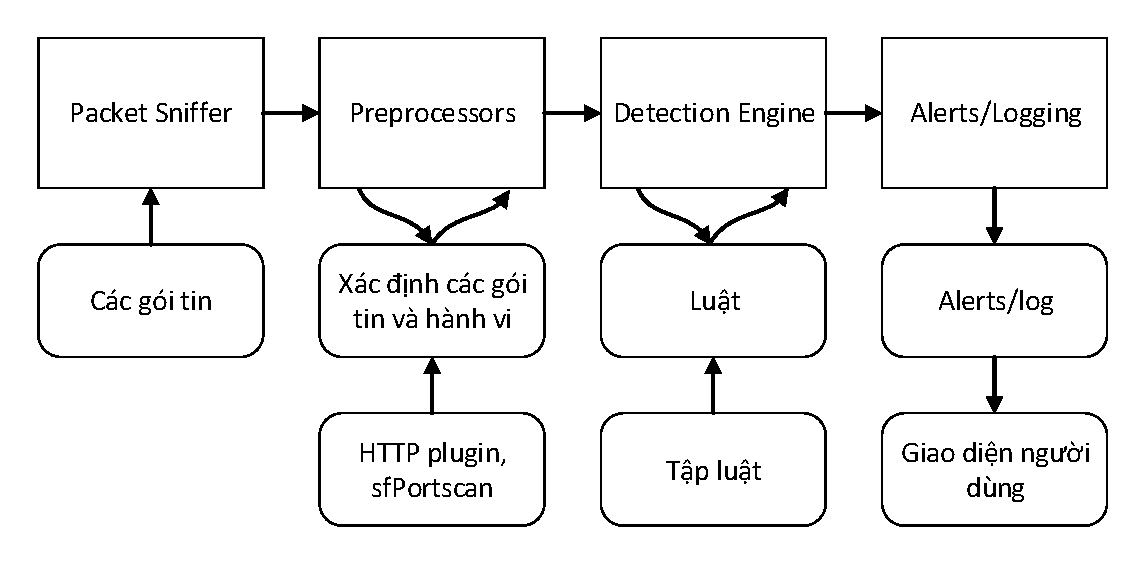
\includegraphics[width=1.0\textwidth]{snort-architecture}
    \caption{
        \label{fig:snort-architecture}
        Kiến trúc của Snort}
\end{figure}

\emph{Thành phần lắng nghe, giải mã gói tin} là một thiết bị phần cứng hoặc phần mềm được đặt trong mạng. Chức năng của nó là phân tích các giao thức thành thông tin mà con người có thể đọc và hiểu được, hỗ trợ giải mã các giao thức khác nhau bao gồm IP, ICMP, TCP, UDP thành dữ liệu các lớp trên.

\emph{Thành phần tiền xử lý} cho phép phân tích cú pháp dữ liệu theo những cách khác nhau. Một số mô-đun hỗ trợ như sau: Frag3 - mô-đun chống phân mảnh gói tin IP, sfPortscan - mô-đun được thiết kế chống lại các cuộc do thám, như quét cổng, xác định dịch vụ, xác định hệ điều hành, Stream5 - mô-đun tái gộp các gói tin ở tầng TCP. Ở thời điểm hiện tại Snort có 24 mô-đun tiền xử lý~\cite{caswell2007snort}.

\emph{Thành phần phát hiện} là một phần của hệ thống phát hiện xâm nhập dựa trên chữ ký. Nó chịu trách nhiệm lấy dữ liệu từ thành phần tiền xử lý và kiểm tra chúng thông qua các luật. Nếu các luật đó khớp với dữ liệu trong gói tin, nó sẽ được gửi tới hệ thống cảnh báo, nếu không nó sẽ bị bỏ qua. Luật là phần quan trọng nhất của Snort, các cú pháp luật của Snort sẽ được giới thiệu thêm ở mục tiếp theo.

Thành phần cuối cùng là \emph{cảnh báo/ghi nhật ký}. Nếu dữ liệu khớp với một luật trong thành phần phát hiện, một cảnh báo sẽ được đưa ra. Các cảnh báo có thể được gửi đến các tập tin nhật ký, gửi qua mạng thông qua SNMP, SMTP hoặc cũng có thể lưu trữ vào cơ sở dữ liệu như MySQL. Giống như thành phần tiền xử lý, chức năng này được cấu hình trong tập tin cấu hình của Snort, có thể chỉ định cảnh báo và ghi lại trong tập tin cấu hình nếu muốn kích hoạt. Snort cũng hỗ trợ nhiều phần mở rộng giúp người quản trị nhận các cảnh báo cũng như phân tích các dữ liệu một cách trực quan. Bảng~\ref{tab:snort-addons} là danh sách một số phần mở rộng cho Snort.

\begin{table}[!htbp]
\centering
\small
\setlength{\extrarowheight}{0.2pt}
\caption{\label{tab:snort-addons}Một số phần mở rộng hỗ trợ cho Snort}
\begin{tabular}{|p{4cm}|p{10.5cm}|}
\hline
\textbf{Tên phần mở rộng}                 & \textbf{Mô tả}                                                                                                                                          \\ \hline
ACID                                      & ACID được biết như một phần mở rộng phân tích cú pháp nhật ký dựa trên PHP, cung cấp khả năng tìm kiếm và là một giao diện phân tích nhật ký của Snort. \\ \hline
SGUIL                                    & Một nền tảng web cung cấp tính năng giám sát và phân tích nhật ký cho Snort.                                                                            \\ \hline
Oinkmaster                             & Một Pert script giúp cập nhật các luật của Snort và có thể đánh dấu những luật không muốn sau mỗi lần cập nhật.                                         \\ \hline
IDS Policy Manager               & Một giao diện quản lý dành cho Windows XP.                                                                                                              \\ \hline
SnortSnarf                               & Một chương trình viết bằng Perl giúp tạo và cung cấp các bản báo cáo log gần đây một cách tổng hợp dưới dạng HTML.                                      \\ \hline
Swatch                                     & Một công cụ giám sát nhật ký hệ thống theo thời gian thực và gửi cảnh báo bằng email.                                                                   \\ \hline
BASE                                      & Một giao diện web cho Snort, cung cấp khả năng truy vấn và cảnh báo cho Snort.                                                                          \\ \hline
\end{tabular}
\end{table}

\subsection{Tập luật}
Snort sử dụng một ngôn ngữ mô tả tập luật đơn giản, nhưng cũng khá hiệu quả và mạnh mẽ. Hầu hết các luật của Snort được viết trên một dòng, và có thể mở rộng thành nhiều dòng bằng ký tự gạch chéo ngược "\textbackslash " ở cuối mỗi dòng. Luật của Snort bao gồm 2 phần: tiêu đề luật (rule header) và tùy chọn luật (rule option)~\cite{snort2017documents}.

\subsubsection{Tiêu đề luật}
\emph{Rule header} gồm 4 phần: Rule action, Protocol, Src/Dst và Port.

\begin{itemize}
\item \emph{Rule action:} Rule action sẽ nói cho Snort biết sẽ làm gì khi tìm thấy gói tin phù hợp với các luật đã định sẵn. Có 5 hành động là: \emph{Alert} - cảnh báo, \emph{Log} - ghi nhật ký, \emph{Pass} - cho qua, \emph{Active} - kích hoạt, \emph{Dynamic} - duy trì trạng thái nhàn rỗi đến khi được kích hoạt.
\item \emph{Protocol:} chỉ ra giao thức mà Snort sẽ phân tích: TCP, UDP, ICMP và IP.
\item \emph{IP address:} địa chỉ IP của nơi đi và nơi đến của 1 gói tin. Ví dụ: \emph{192.168.1.1 \tab 192.168.2.1} cho biết địa chỉ nguồn là 192.168.1.1 và địa chỉ đích là 192.168.2.1.
\item \emph{Port:} số hiệu cổng dịch vụ mà Snort sẽ phân tích. Ví dụ: 80 của HTTP, 22 của SSH.
\end{itemize}

\subsubsection{Các tùy chọn luật}
\emph{Rule option} là trung tâm của việc phát hiện xâm nhập. Nội dung của nó chứa các dấu hiệu để xác định một cuộc xâm nhập. Rule option nằm ngay sau Rule header và được bao bọc bởi dấu ngoặc đơn "\(()\)". Tất cả Rule option được ngăn cách nhau bởi dấu chấm phẩy "\(;\)", phần đối số sẽ được phân cách nhau bởi dấu hau chấm "\(:\)".

Có bốn loại Rule option chính bao gồm:
\begin{itemize}
\item \emph{General:} gồm các tùy chọn cung cấp thông tin về luật đó nhưng không có bất cứ ảnh hưởng nào trong quá trình phát hiện.
\item \emph{Payload:} gồm các tùy chọn liên quan đến phần tải của gói tin.
\item \emph{Non-payload:} gồm các tùy chọn không liên quan đến phần tải của gói tin.
\item \emph{Post-detection:} gồm các tùy chọn áp dụng một luật cụ thể sau khi một luật được bỏ qua.
\end{itemize}

\subsubsection*{\textit{a) General}}

\begin{itemize}
\item \emph{Msg:} gán thêm một chuỗi văn bản vào nhật ký và cảnh báo. Chuỗi đó được đặt trong dấu ngoặc kép \(" "\). Ví dụ: \emph{msg: "Hello World"}.
\item \emph{Reference:} dùng khi muốn tham chiếu thông tin từ một hệ thống khác trên internet.
\item \emph{Sid:} được dùng để xác định duy nhất một luật trong Snort.
\item \emph{Rev:} được sử dụng để định danh các sửa đổi trong luật của Snort, thường dùng để phân biệt các phiên bản luật khác nhau.
\item \emph{Classtype:} được dùng để phân loại các hình thức tấn công kèm theo độ ưu tiên của loại tấn công đó và được định nghĩa trong tập tin \emph{classification.config}.
\item \emph{Priority:} được sử dụng để gán độ nghiêm trọng của một luật.
\end{itemize}

\subsubsection*{\textit{b) Payload}}

\begin{itemize}
\item \emph{Content:} cho phép tìm kiếm các chuỗi cụ thể trong phần tải của gói tin (payload) và kích hoạt các cảnh báo dựa trên các dữ liệu đó. Nội dung có thể ở dạng nhị phân hoặc ASCII. Ví dụ: \emph{content: "GET"}
\item \emph{Nocase:} kết hợp với từ khóa content để tìm kiếm chuỗi mà không phân biệt hoa thường.
\item \emph{Rawbyte:} cho phép các luật xem các gói dữ liệu thô chưa được giải mã.
\item \emph{Depth:} dùng để xác định khoảng cách bao xa mà luật đó sẽ tìm tới, tối thiểu là 1 và tối đa là 65535. Nó được dùng với từ khóa content để giới hạn nội dung tìm kiếm.
\item \emph{Offset:} dùng để xác định điểm bắt đầu tìm kiếm, cho phép giá trị từ \emph{-65535} đến \emph{65535}.
\item \emph{Distance:} được sử dụng trong trường hợp muốn bỏ qua bao nhiêu byte từ nội dung tìm kiếm trước đó.
\item \emph{Within:} được dùng để đảm bảo rằng có nhiều nhất N byte giữa các mẫu nội dung tìm kiếm.
\item \emph{Uricontent:} tương tự như content nhưng để tìm kiếm chuỗi trong URI.
\end{itemize}

\subsubsection*{\textit{c) Non-Payload}}

\begin{itemize}
\item \emph{Ttl:} dùng để kiểm tra giá trị \emph{time-to-live} trong tiêu đề gói tin IP. Được sử dụng để phát hiện hành động quét mạng. Cấu trúc:
\\ \tab \emph{Ttl:[ <,>,=,<=,>=]<number;} - ví dụ: \emph{ttl:<3}
\\ \tab \emph{Ttl:[ <number>]-[<number>];} - ví dụ: \emph{ttl:2-3}
\item \emph{Tos:} kiểm tra trường \emph{ToS (type of service)} trong tiêu đề gói tin IP.
\item \emph{Id:} được sử dụng để kiểm tra các giá trị cụ thể trong trường ID của tiêu đề gói tin IP.
\item \emph{Ipopts:} được sử dụng để kiểm tra trường \emph{IP option} trong tiêu đề gói tin IP.
\item \emph{Fragbits:} được sử dụng để kiểm tra sự phân mảnh và \emph{bit reserved} trong trường 3 bit Flags của tiêu đề gói tin IP.
\item \emph{Dsize:} dùng để kiểm tra kích thước của phần dữ liệu trong gói tin.
\item \emph{Flag:} sử dụng để kiểm tra các bit trong trường TCP Flag của tiêu đề gói tin TCP. Các bit này gồm: \emph{F - FIN, S - SYN, R - RST, P - PSH, A - ACK, U - URG}.
\item \emph{Flow:} áp dụng vào luật có gói tin di chuyển theo một hướng cụ thể. Các tùy chọn bao gồm: \emph{to\_client}, \emph{to\_server}.
\item \emph{Sed:} dùng để kiểm tra \emph{sequence number} của tiêu đề gói tin TCP.
\item \emph{Ack:} dùng để kiểm tra giá trị \emph{acknowledge number} của tiêu đề gói tin TCP.
\item \emph{Window:} dùng để kiểm tra kích cỡ cửa sổ trong tiêu đề gói tin TCP.
\item \emph{Icmp\_id:} dùng để kiểm tra giá trị ID của tiêu đề gói tin ICMP.
\item \emph{Icmp\_seq:} dùng để kiểm tra giá trị \emph{sequence} của tiêu đề gói tin ICMP.
\item \emph{Rpc:} dùng để phát hiện các yêu cầu dựa trên RPC.
\item \emph{Sameip:} dùng để kiểm tra địa chỉ nguồn và địa chỉ đích có giống nhau không.
\end{itemize}

\subsubsection*{\textit{d) Post-detection}}

\begin{itemize}
\item \emph{Logto:} dùng để ghi nhật ký vào các tập tin đặc biệt. ví dụ: \emph{logto:logto\_log}.
\item \emph{Session:} dùng để trích xuất thông tin người dùng từ một phiên TCP.
\item \emph{Resp:} cho phép chủ động tạo ra những phản hồi trước các vi phạm.
\item \emph{React:} cho phép tạo ra các phản hồi bao gồm gửi một trang web hoặc mội nội dung nào đó tới client và sau đó đóng kết nối lại.
\item \emph{Tag:} cho phép các luật ghi nhiều hơn một gói tin khi luật đó được kích hoạt.
\item \emph{Detection\_filter:} định nghĩa một mức ngưỡng được phép thực thi bởi địa chỉ nguồn hoặc địa chỉ đích trước khi một luật phát sinh một sự kiện.
\item \emph{Threshold:} sử dụng để quy định một giới hạn nào đó mà các luật của Snort sẽ đưa ra cảnh báo.
\end{itemize}

\begin{leftbar}
\noindent Qua những tóm tắt trên đây, đồ án đã cung cấp một số kiến thức quan trọng về Snort và tập luật của nó. Một số luật cụ thể phục vụ cho hệ thống WIDS đề xuất, đồ án xin được mô tả thêm ở Phụ lục B.
\end{leftbar}

\section{Hệ điều hành OpenWrt}
\subsection{Giới thiệu}
OpenWrt là một bản phân phối Linux nhúng giành cho thiết bị định tuyến không dây, do kiến trúc cũng như hoạt động tương tự một firmware, nên nó thường được gọi là firmware OpenWrt. OpenWrt cung cấp một firmware tối thiểu với khả năng tùy biến cao thông qua các gói bổ sung. OpenWrt gồm các thành phần chính là Linux, util-linux, uClibc/musl và BusyBox. Tất cả các thành phần này được tối ưu về kích thước, đủ nhỏ để để vừa với kích thước lưu trữ và bộ nhớ giới hạn của một thiết bị định tuyến.

Người dùng có thể cấu hình OpenWrt thông qua giao diện dòng lệnh (ash shell) hoặc giao diện web (LuCI). Giống như các bản phân phối Linux khác, OpenWrt sử dụng một hệ quản lý gói có tên là opkg với khoảng 3500 gói phần mềm có sẵn~\cite{openwrt2017wiki}.

OpenWrt có khả năng tương thích với hầu hết phần cứng thiết bị của các hãng, thậm chí có thể cài đặt OpenWrt lên máy tính cá nhân có kiến trúc x86. OpenWrt cũng cung cấp một bộ công cụ hoàn chỉnh hỗ trợ biên dịch chéo, vì vậy hoàn toàn có thể biên dịch nó trên một máy tính có kiến trúc x86, x86\_64 và sau đó cài đặt lên một thiết bị nhúng.

\subsection{Môi trường OpenWrt Buildroot}
Kích thước bộ nhớ flash của thiết bị AP thường khá nhỏ. Thêm vào đó, OpenWrt định dạng bộ nhớ flash thành các phân vùng, trong đó phân vùng chứa firmware là phân vùng "\emph{chỉ đọc}"~\cite{openwrt2017wiki}. Do vậy việc tự xây dựng một firmware với một số phần mềm cần thiết được tích hợp sẵn, khi cài đặt sẽ đưa chúng vào phân vùng chứa firmware, điều này giúp việc sử dụng bộ nhớ flash hiệu quả hơn.

OpenWrt Buildroot cho phép biên dịch một firmware tùy biến cho các phần cứng, kiến trúc được hỗ trợ. Môi trường OpenWrt Buildroot là một loạt các công cụ hỗ trợ biên dịch chéo. Hình~\ref{fig:openwrt-buildroot} thể hiện kiến trúc của OpenWrt Buildroot~\cite{jin2013openwrt}. Các thư mục ở hàng thứ ba trong hình, được tạo ra trong quá trình buildroot.

\begin{figure}[H]
    \centering
    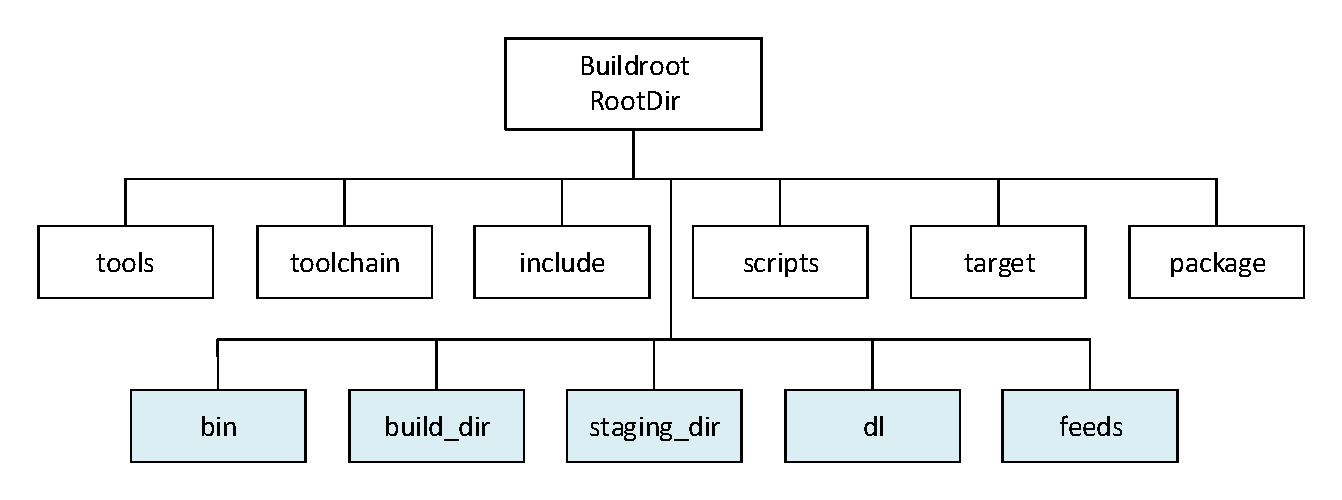
\includegraphics[width=1.0\textwidth]{openwrt-buildroot}
    \caption{
        \label{fig:openwrt-buildroot}
        Kiến trúc của OpenWrt Buildroot}
\end{figure}

Trong đó:
\begin{itemize}
\item \emph{tools} -- bao gồm tất cả các chỉ thị xây dựng để lấy về các công cụ xây dựng firmware.
\item \emph{toolchain} {-­‐} bao gồm các tất cả các chỉ thị xây dựng để lấy về tiêu đề nhân Linux, thư viện C, bin{-}utils, trình biên dịch và trình gỡ rối.
\item \emph{target} {-­‐} các chỉ thị xây dựng cho quá trình tạo bản chụp firmware và cho quá trình xây dựng nhân; biên dịch nhân và xây dựng bản chụp firmware.
\item \emph{package} -- OpenWrt Makefile và các bản vá cho tất cả các gói chính thức.
\item \emph{scripts} -- các script perl của hệ quản lý gói OpenWrt.
\item \emph{dl} -- thư mục chứa tất cả các gói tin cài đặt được tải về.
\item \emph{build\_dir} --  thư mục chứa các công cụ phục vụ người dùng được biên dịch chéo.
\item \emph{staging\_dir} -- thư mục chứa các công cụ biên dịch chéo.
\item \emph{feeds} -- thư mục chứa các cấu hình nguồn cài đặt.
\item \emph{bin} -- thư mục  chứa các bản chụp firmware sau biên dịch và tất cả các gói \emph{.ipk} được tạo ra.\\
\end{itemize}

Sau khi OpenWrt Buildroot được cấu hình thích hợp, nền tảng và kiến trúc đích được xác định, các gói phần mềm cho người dùng được lựa chọn, OpenWrt Buildroot sẽ thực hiện quá trình xây dựng firmware qua các bước chính như sau:

1. Tải về các công cụ biên dịch chéo, tiêu đề nhân, và các công cụ tương tự.

2. Thiết lập thư mục cho giai đoạn (\emph{staging\_dir/}). Đây là nơi mà các công cụ biên dịch chéo sẽ được cài đặt.   

3. Tạo thư mục tải về (mặc định là \emph{dl/}). Đây là nơi mà các gói cài đặt được tải về. 

4. Tạo thư mục xây dựng (\emph{build\_dir/}). Đây là nơi mà tất cả các công cụ phục vụ người dùng được biên dịch.

5. Tạo thư mục đích (mặc định là \emph{build\_dir/target-arch/root}) và bộ khung của tập tin hệ thống. Thư mục này sẽ chứa tập tin hệ thống cuối cùng. 

6. Cài đặt các gói phục vụ người dùng vào tập tin hệ thống gốc và nén toàn bộ tập tin hệ thống gốc với định dạng phù hợp. Bản chụp firmware cuối cùng được tạo trong \emph{bin/}.

\section{Kết chương}
Trong chương 2, đồ án đã trình bày về những kiến thức nền tảng và các kiến thức liên quan cho việc xây dựng đề tài. Qua đó, các phương pháp phát hiện xâm nhập nói chung và phát hiện xâm nhập trong mạng không dây nói riêng đã được làm rõ. Việc khảo sát các hệ thống đã được phát triển đã mang lại cái nhìn tổng quan về một số hệ thống phát hiện xâm nhập mạng không dây trên thế giới, cũng như thấy được ưu nhược điểm của chúng. Đồ án cũng nghiên cứu về Kismet Wireless và Snort, là những phần mềm phát hiện xâm nhập mã nguồn mở điển hình và đang được ứng dụng rộng rãi.

Từ những kết quả nghiên cứu nêu trên, đồ án sẽ thực hiện một ý tưởng đó là xây dựng một hệ thống phát hiện xâm nhập mạng không dây dựa trên sự kết hợp những tính năng nổi bật của Kismet Wireless và Snort, chi tiết thiết kế và hoạt động của hệ thống sẽ được trình bày ở chương tiếp theo.

\chapter{THIẾT KẾ HỆ THỐNG}
\ifpdf
    \graphicspath{{Chapter3/Chapter3Figs/PNG/}{Chapter3/Chapter3Figs/PDF/}{Chapter3/Chapter3Figs/}}
\else
    \graphicspath{{Chapter3/Chapter3Figs/EPS/}{Chapter3/Chapter3Figs/}}
\fi

\section{Hướng tiếp cận}
Hình~\ref{fig:wids-traditional} là một giải pháp triển khai hệ thống IDS truyền thống cho mạng không dây. Trong đó:

\begin{itemize}
\item Router: định tuyến và cung cấp kết nối từ mạng nội bộ ra Internet.
\item Switch: được cấu hình kỹ thuật SPAN trên cổng nối ra NIDS. Kỹ thuật này cho phép Switch tự động sao chép các gói tin từ các cổng khác đến cổng giám sát, như vậy toàn bộ lưu thông trong mạng đều được gửi đến NIDS.
\item NIDS: hệ thống phát hiện xâm nhập mạng, giám sát toàn bộ lưu lượng trong mạng có dây và mạng không dây.
\item AP: cung cấp kết nối ra Internet cho các STA.
\item STA: các thiết bị sử dụng mạng không dây.
\end{itemize}

\begin{figure}[H]
    \centering
    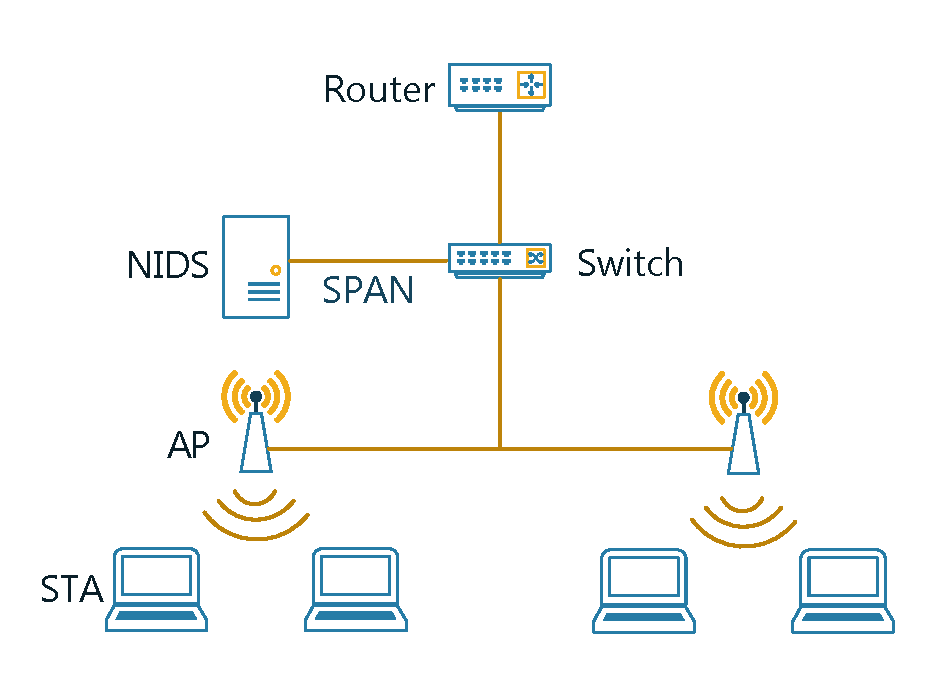
\includegraphics[width=0.8\textwidth]{wids-traditional}
    \caption{
        \label{fig:wids-traditional}
        Giải pháp IDS truyền thống cho mạng không dây}
\end{figure}

Giải pháp này có ưu điểm đó là hệ thống IDS có thể kiểm soát toàn bộ lưu thông vào và ra của mạng không dây. Tuy nhiên, nó không thể kiểm soát liên lạc nội bộ giữa các STA không dây, vì những lưu lượng này không đi qua Switch cũng như NIDS. Giải pháp này cũng không phát hiện được các tấn công từ bên ngoài vào mạng không dây. Ngoài ra, NIDS sẽ phải làm việc với lưu lượng mạng rất lớn, từ cả mạng có dây và mạng không dây, dó đó sẽ ảnh hưởng đến hiệu năng giám sát và phát hiện xâm nhập của NIDS.

Để giám sát các tấn công từ bên ngoài vào mạng không dây, hệ thống sẽ cần thêm các cảm biến không dây (Wireless Sensor). Cảm biến không dây có nhiệm vụ lắng nghe các khung được truyền trong phạm vi thu sóng của nó, sau đó chuyển về máy chủ IDS để xử lý. Như vậy, ngoài các AP để cung cấp kết nối cho các STA, sẽ cần phải có thêm các cảm biến không dây, làm cho chi phí triển khai một hệ thống WIDS tăng lên khá nhiều.

Từ những trở ngại như trên, đồ án xin đưa ra một hướng tiếp cận mới để triển khai một hệ thống WIDS gọi là KMA-WIDS, bằng cách sử dụng các AP như các cảm biến không dây. Các AP này sẽ thu thập các khung quản lý không được mã hóa, để phát hiện các tấn công từ bên ngoài vào mạng không dây. Đồng thời, chúng được cấu hình để tự động sao chép tất cả các gói tin trong mạng không dây và gửi đến cho máy chủ IDS để có thể phát hiện các tấn công bên trong mạng không dây. Hình~\ref{fig:diagram-wids-new} mô tả kiến trúc của hệ thống KMA-WIDS. Các thông tin mà AP thu thập được gửi tới máy chủ IDS, tại đây chúng được xử lý và phát hiện các tấn công, hệ thống sẽ tạo ra các cảnh báo đến giao diện quản trị trên nền tảng web khi phát hiện các tấn công. Ưu điểm của hệ thống này là ứng dụng các phần mềm mã nguồn mở, mang lại một hệ thống WIDS phù hợp về chi phí và hiệu năng.

\begin{figure}[H]
    \centering
    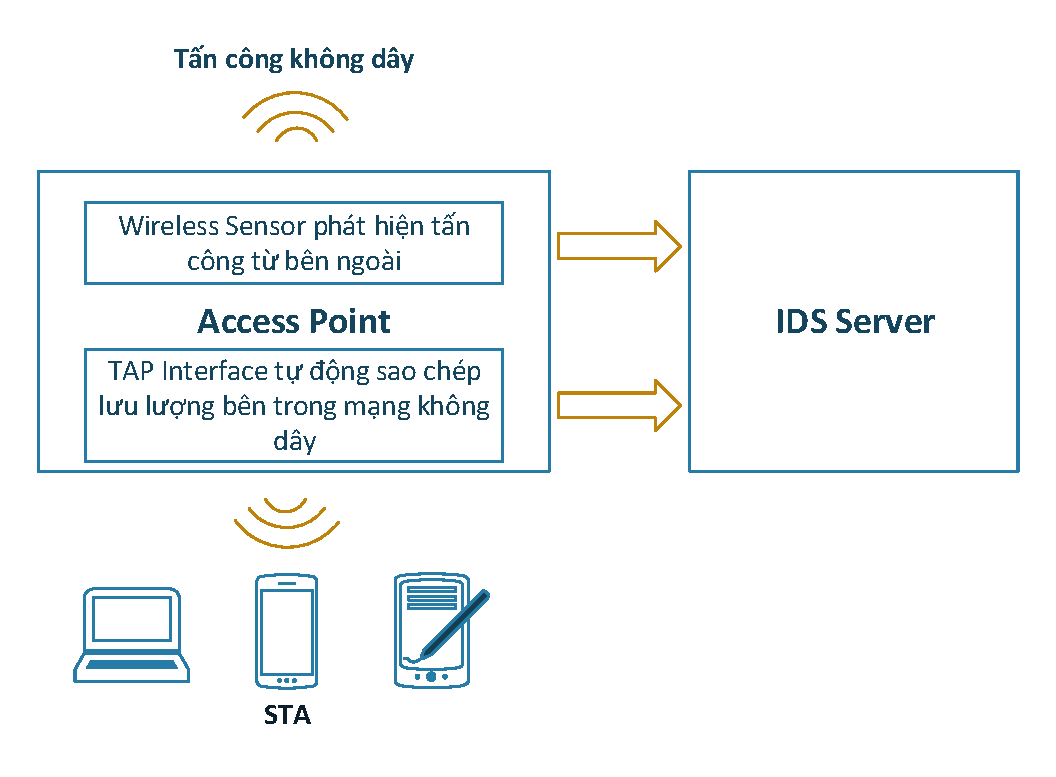
\includegraphics[width=0.85\textwidth]{diagram-wids-new}
    \caption{
        \label{fig:diagram-wids-new}
        Giải pháp KMA-WIDS}
\end{figure}

\section{Các thành phần chính}
Hệ thống WIDS được đề xuất bao gồm hai thiết bị vật lý, một Access Point TP-Link chạy hệ điều hành OpenWrt và một IDS Server dùng máy tính nhúng Raspberry Pi~\cite{rasberry2017raspberry} chạy hệ điều hành Raspbian~\cite{raspberry2017raspbian}. Hình~\ref{fig:diagram-wids-new-components} thể hiện vị trí cụ thể của từng phần mềm trong hệ thống WIDS đề xuất. Cụ thể như sau:

\begin{itemize}
\item OpenWrt: đây sẽ là hệ điều hành mà đồ án chọn để thay thế firmware gốc của AP, như đã trình bày ở chương 2, OpenWrt cung cấp một firmware tối thiểu với khả năng mở rộng cao thông qua việc cài đặt các phần mềm bổ sung.
\item Raspbian: máy tính nhúng Raspberry Pi sẽ được cài đặt Raspbian, một hệ điều hành được tối ưu dựa trên nền tảng Debian, cung cấp một bản Linux rút gọn với đầy đủ chức năng và tương thích với máy tính nhúng Raspberry Pi.

\begin{figure}[H]
    \centering
    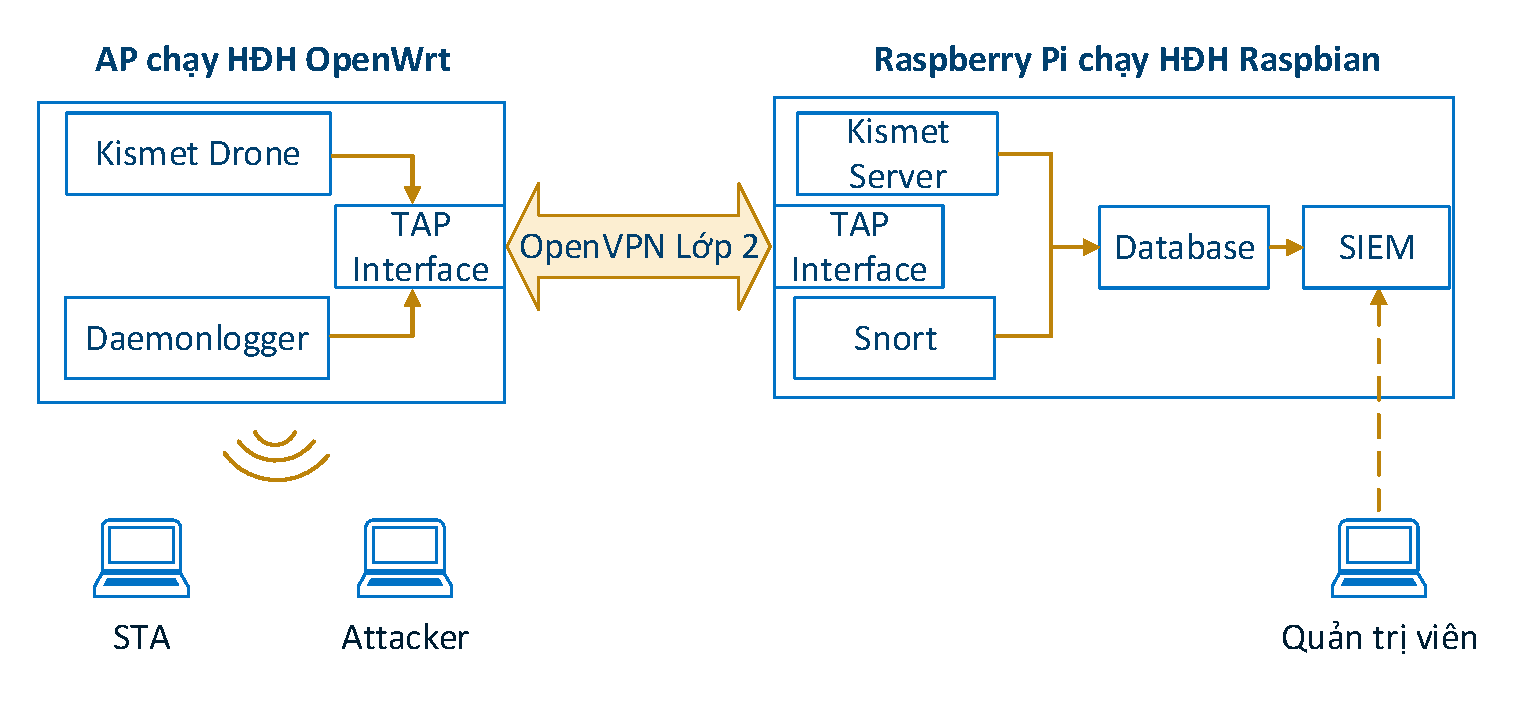
\includegraphics[width=1.0\textwidth]{diagram-wids-new-components}
    \caption{
        \label{fig:diagram-wids-new-components}
        Vị trí các phần mềm trong KMA-WIDS}
\end{figure}

\item Kismet Drone: là gói phần mềm được cài đặt lên OpenWrt để làm nhiệm vụ của một WIDS Sensor, thu thập các khung để hỗ trợ cho việc phát hiện các tấn công từ bên ngoài.
\item Kismet Server: đáp ứng kiến trúc phân tán của Kismet, Kismet Server được cài đặt trên IDS Server để nhận các khung từ Kismet Drone, có nhiệm vụ phát hiện các tấn công từ bên ngoài mạng không dây.
\item Daemonlogger~\cite{martin2008daemonlogger}: là gói phần mềm được cài đặt lên OpenWrt, hoạt động như một "software tap", tự động sao chép các gói tin từ giao diện mạng không dây và gửi về IDS Server qua giao diện mạng ảo TAP interface, hỗ trợ cho việc phát hiện các tấn công bên trong mạng không dây.
\item Snort: gói phần mềm được cài đặt trên IDS Server. Snort sẽ lắng nghe trên TAP interface để nhận các gói tin do Daemonlogger gửi về. Với chế độ hoạt động NIDS, Snort mang lại khả năng phát hiện các tấn công từ bên trong mạng không dây.
\item Database: hệ thống cũng cung cấp khả năng lưu trữ các sự kiện vào cơ sở dữ liệu, thông qua gói phần mềm MySQL~\cite{rasberry2017raspberry} để làm hệ quản trị cơ sở dữ liệu. Ngoài ra, để chuyển đổi định dạng các sự kiện xử lý bằng Kismet Server và Snort thành một định dạng thống nhất, gói phần mềm Barnyard2~\cite{ian2016barnyard2} và Sagan~\cite{quadrant2017sagan} cũng được sử dụng.
\item SIEM (Security Information and Event Management): là một hệ thống quản lý sự kiện an ninh. Trong hệ thống KMA-WIDS, sẽ sử dụng gói phần mềm Snorby~\cite{community2017snorby} được triển khai trên nền Apache HTTP Server~\cite{apache2017apache} để cung cấp một giao diện web quản lý sự kiện an ninh cho hệ thống.
\item OpenVPN~\cite{vpn2017documentation}: gói phần mềm này sẽ được cài đặt và cấu hình ở cả hai thiết bị, nó sẽ tạo ra một kết nối VPN lớp 2 thông qua TAP interface để hỗ trợ cho việc truyền dữ liệu an toàn cho hệ thống WIDS. Đồng thời, còn một số lý do khác mà hệ thống yêu cầu một kết nối VPN lớp 2, sẽ được trình bày ở phần sau.
\item Ngoài ra, hệ thống cũng sử dụng nhiều script để tự động hóa quá trình khởi chạy các phần mềm khi khởi động hệ thống, cũng như một số công cụ và thư viện phụ thuộc để hệ thống có thể hoạt động hoàn chỉnh. 
\end{itemize}

\section{Thiết kế và hoạt động}
\subsection{Thiết bị Access Point}
\subsubsection{Tổng quan}
Để có thể triển khai hệ thống KMA-WIDS, cần sử dụng một thiết bị Access Point có dung lượng bộ nhớ flash trên 8~MB. Vì vậy dòng sản phẩm được đồ án lựa chọn thử nghiệm là TP-Link TL-WR1043ND. Dòng sản phẩm Access Point này có dung lượng bộ nhớ flash từ 8 MB, bộ nhớ RAM từ 32 MB; sử dụng vi mạch không dây Qualcomm Atheros với khả năng hỗ trợ hầu hết các chuẩn WiFi. Nó cũng hỗ trợ 5 cổng Ethernet với tốc độ Gigabit, trong đó 1 cổng dùng để làm kết nối WAN, cung cấp liên lạc ra Internet cho các cổng mạng và kết nối WiFi~\cite{openwrt2017tplink}. 

Đồ án sẽ thực hiện xây dựng một firmware tích hợp và cài đặt thay thế lên Access Point. Firmware OpenWrt là một bản phân phối Linux tối thiểu, do vậy chúng cung cấp khả năng quản lý khá dễ dàng. Sơ đồ kiến trúc bên trong thiết bị được mô tả như Hình~\ref{fig:tp-link-wr1043nd}~\cite{openwrt2017tplink}. Dựa vào sơ đồ, ta có thể thấy OpenWrt ánh xạ các card mạng vật lý thành các giao diện mạng luận lý để quản lý, trong đó:

\begin{itemize}
\item \emph{wlan0}: giao diện mạng đại diện cho card mạng WiFi.
\item \emph{eth1}: giao diện mạng trên Switch để kết nối \emph{wlan0} với Switch. Switch ở đây là một thành phần được tích hợp sẵn bên trong của thiết bị.

\begin{figure}[H]
    \centering
    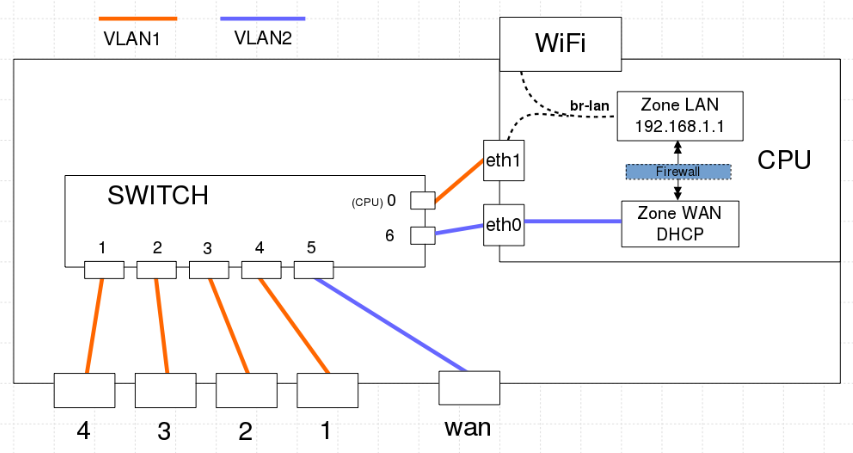
\includegraphics[width=1.0\textwidth]{tp-link-wr1043nd}
    \caption{
        \label{fig:tp-link-wr1043nd}
        Kiến trúc bên trong TP-Link TL-WR1043ND}
\end{figure}

\item \emph{br-lan}: giao diện mạng có nhiệm vụ tạo cầu nối giữa các cổng thuộc VLAN1 trên Switch (\emph{eth1}) với \emph{wlan0} nhằm tạo nên một giao diện mạng chung để kiểm soát truy cập ra Internet, cũng như cho phép các máy tính có dây có thể liên lạc với các STA của mạng WiFi.
\item \emph{eth0}: giao diện mạng trên Switch để cung cấp kết nối ra Internet cho toàn bộ thiết bị, được kiểm soát truy cập thông qua firewall. \emph{eth0} thuộc VLAN2, nên có thể nói nó hoàn toàn độc lập với các cổng thuộc VLAN1 trên Switch.
\item Các cổng trên Switch: được sử dụng để cung cấp kết nối cho các máy tính có dây.
\end{itemize}

\subsubsection{Phương pháp thu thập các khung}
Sau khi thay thế bằng firmware OpenWrt, card mạng không dây của thiết bị TP-Link TL-WR1043ND sử dụng trình điều khiển \emph{mac80211} thông qua gói \emph{kmod-mac80211}~\cite{openwrt2017wiki}. Trình điều khiển \emph{mac80211} cho phép card mạng không dây cùng một lúc có thể hoạt động ở hai chế độ: chế độ Access Point để phát sóng WiFi, chế độ giám sát cho phép lắng nghe và thu thập các khung truyền trong phạm vi thu phát sóng~\cite{steven2015capturing}. Vì đặc điểm này, Kismet Drone khi khởi chạy, sẽ tạo ra một giao diện mạng ảo ở chế độ giám sát là \emph{wlan0mon}, sau đó nó sẽ thu thập các khung thông qua giao diện mạng này, và gửi tới cho Kismet Server trên IDS Server. Giao diện mạng \emph{wlan0} hoạt động ở chế độ Access Point, cung cấp kết nối WiFi cho các STA như bình thường.

\subsubsection{Phương pháp sao chép lưu lượng không dây}
Các cổng trên Switch của Access Point sử dụng chung một giao diện mạng để truy cập ra Internet, đó là \emph{eth1}. Điều này tạo nên một khó khăn khi thực hiện sao chép các lưu lượng không dây từ card mạng không dây, và đẩy đến một cổng cụ thể trên Switch, cổng mà sẽ nối với IDS Server. Khi lưu lượng được gửi đến \emph{eth1}, toàn bộ các cổng trên Switch đều nhận được các lưu lượng này. Các lưu lượng này không yêu cầu được định tuyến hay chuyển mạch, vì vậy việc gửi toàn bộ các cổng sẽ khiến hiệu năng mạng bị ảnh hưởng. Hơn nữa, trong trường hợp này, AP và IDS Server phải kết nối trực tiếp, không thông qua thiết bị nào khác thì mới áp dụng được.

Vấn đề trên đây có hai hướng giải quyết. Cách thứ nhất là thực hiện cấu hình tạo thêm một VLAN3, xóa một cổng cụ thể thuộc VLAN1 và thêm nó vào VLAN3, cổng này sẽ trở thành một cổng quản lý, dùng để kết nối trực tiếp với IDS Server, các lưu lượng trong VLAN3 sẽ độc lập hoàn toàn với hai VLAN còn lại của Switch. Cách thứ hai là thực hiện cấu hình một kết nối VPN lớp 2 giữa Access Point với IDS Server, một kết nối VPN lớp 2 sẽ tạo nên hai giao diện mạng TAP ở hai đầu, giúp cho việc đẩy dữ liệu đến đúng IDS Server thông qua giao diện mạng TAP. Trong cách thứ nhất, có nhược điểm đó là cổng quản lý là một cổng cố định, phải được đánh dấu để tránh nhầm lẫn, bên cạnh đó AP và IDS Server còn phải kết nối trực tiếp với nhau để đảm bảo lưu lượng mạng sao chép đi đúng đến IDS Server. Cách thứ hai mang lại ưu điểm về khả năng linh hoạt và bảo mật, có thể sử dụng bất cứ cổng nào thuộc VLAN1 của thành phần Switch để nối với IDS Server, kết nối VPN lớp 2 sẽ phụ trách phần còn lại, hơn nữa lưu lượng quản lý lúc này được bảo vệ bởi kết nối VPN. Vì những ưu điểm như vậy, đồ án quyết định triển khai theo hướng giải quyết thứ hai, cấu hình một kết nối VPN lớp 2 giữa Access Point và IDS Server.

Một số thiết bị Switch thường có một cổng đặc biệt, gọi là cổng quản lý. Cổng quản lý có thể được cấu hình kỹ thuật SPAN, với tính năng là tự động sao chép tất cả các gói tin lưu thông qua Switch và đẩy về cổng quản lý, phục vụ mục đích giám sát hệ thống mạng, xử lý sự cố. Trong thiết bị Access Point, giao diện mạng không dây không phải là một cổng trên thành phần Switch nên không thể làm được điều này, vì vậy đồ án sẽ sử dụng một phần mềm mã nguồn mở có tên là Daemonlogger, nó có chức năng là sao chép các gói tin từ một giao diện mạng, và đẩy về một giao diện mạng khác. Daemonlogger được viết bởi Martin Roeschi, cũng là tác giả của phần mềm Snort nổi tiếng, thuộc sở hữu của Sourcefire và nay là Cisco~\cite{martin2008daemonlogger}. Daemonlogger là một phần mềm dựa trên thư viện phân tích mạng libpcap, hoạt động của thư viện libpcap được thể hiện trong Hình~\ref{fig:libpcap-works}. Có thể thấy một gói tin nhận được từ bên gửi sẽ được tái tạo hoàn chỉnh ở bên nhận, có nghĩa là sẽ không còn các mã hóa đường truyền. Chính khả năng này làm cho libpcap được sử dụng rộng rãi trong các công cụ phân tích mạng như Snort, tcpdump. Libpcap cũng cho phép sử dụng bộ lọc BPF (Berkeley Packet Filter) để áp dụng những cú pháp lọc lên gói tin thu thập, giúp giảm thiểu lưu lượng cần phân tích.

\begin{figure}[H]
    \centering
    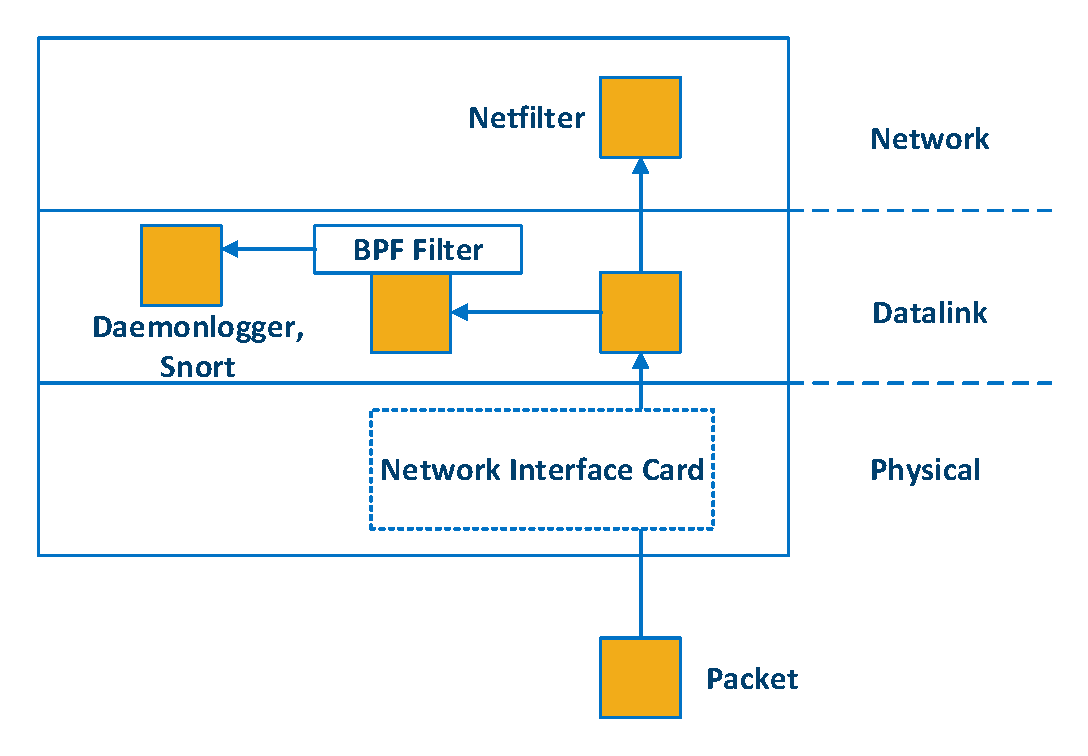
\includegraphics[width=0.9\textwidth]{libpcap-works}
    \caption{
        \label{fig:libpcap-works}
        Hoạt động của libpcap}
\end{figure}

\subsection{Thiết bị máy tính nhúng Raspberry Pi}
\subsubsection{Tổng quan}

Raspberry Pi là một dòng máy tính nhỏ gọn, chỉ bao gồm một bảng mạch có kích thước tương tự như thẻ tín dụng thông thường. 
Hình~\ref{fig:Raspberry-Pi-2-Model-B-1GB} là hình ảnh về các thành phần của một máy tính nhúng Raspberry Pi 2 mẫu B, phiên bản mà đồ án sử dụng. Phiên bản này sử dụng vi xử lý 900~MHz lõi tứ ARM Cortex~-~A7, và bộ nhớ RAM~1GB~\cite{rasberry2017raspberry}. Máy tính nhúng sử dụng hệ điều hành Raspbian, một phiên bản tối ưu dựa trên Debian, cung cấp môi trường Linux chuẩn, đáp ứng nhu cầu sử dụng máy tính cơ bản. Ngoài ra, Raspberry Pi cũng được thiết kế để vận hành liên tục trong thời gian dài, với mức tiêu thụ năng lượng rất thấp~\cite{wikipedia2017raspberry}. Trong đồ án này, máy tính nhúng Raspberry Pi sẽ được cài đặt để làm một IDS Server. Trên đó sẽ cài đặt các phần mềm đảm nhiệm các chức năng cụ thể như mô tả phần mềm ở phần đầu. Sau đây là các luồng xử lý dữ liệu chính mà IDS Server thực hiện.

\begin{figure}[H]
    \centering
    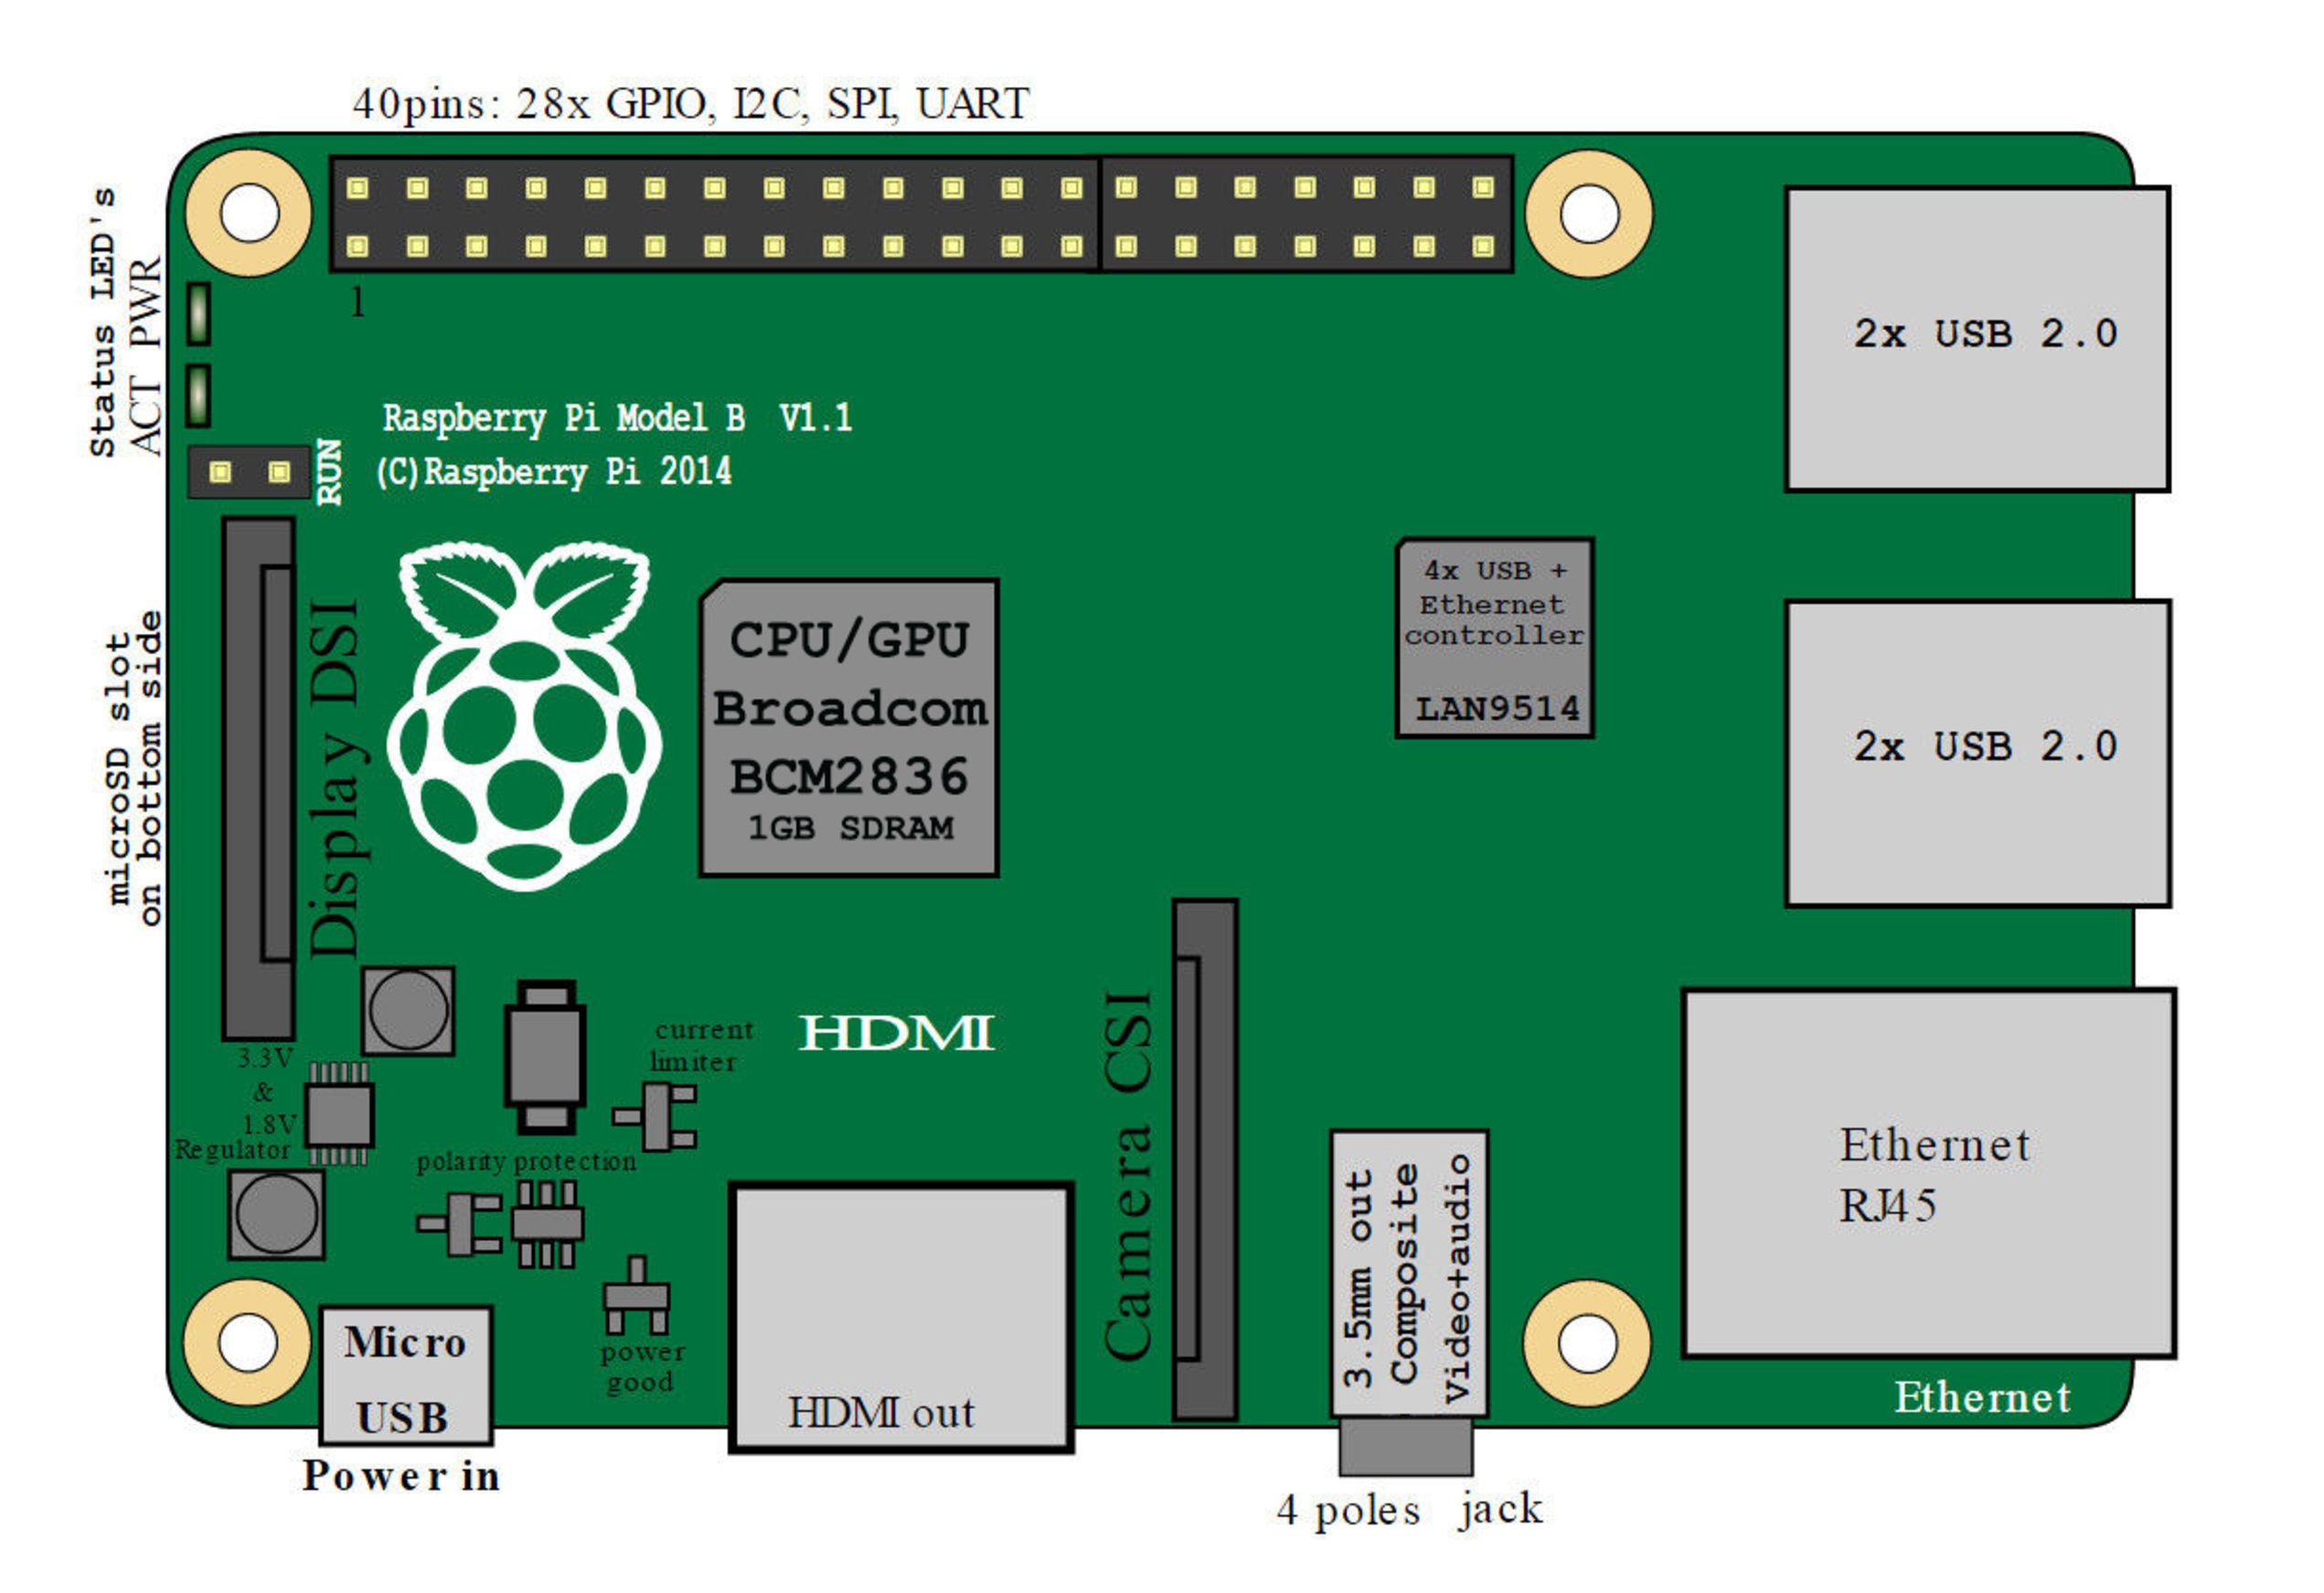
\includegraphics[width=0.9\textwidth]{Raspberry-Pi-2-Model-B-1GB}
    \caption{
        \label{fig:Raspberry-Pi-2-Model-B-1GB}
        Máy tính nhúng Raspberry Pi 2 mẫu B}
\end{figure}

\subsubsection{Luồng xử lý dữ liệu của Kismet}
Luồng xử lý dữ liệu của Kismet được mô tả như Hình~\ref{fig:kismet-workflow}.

\begin{figure}[H]
    \centering
    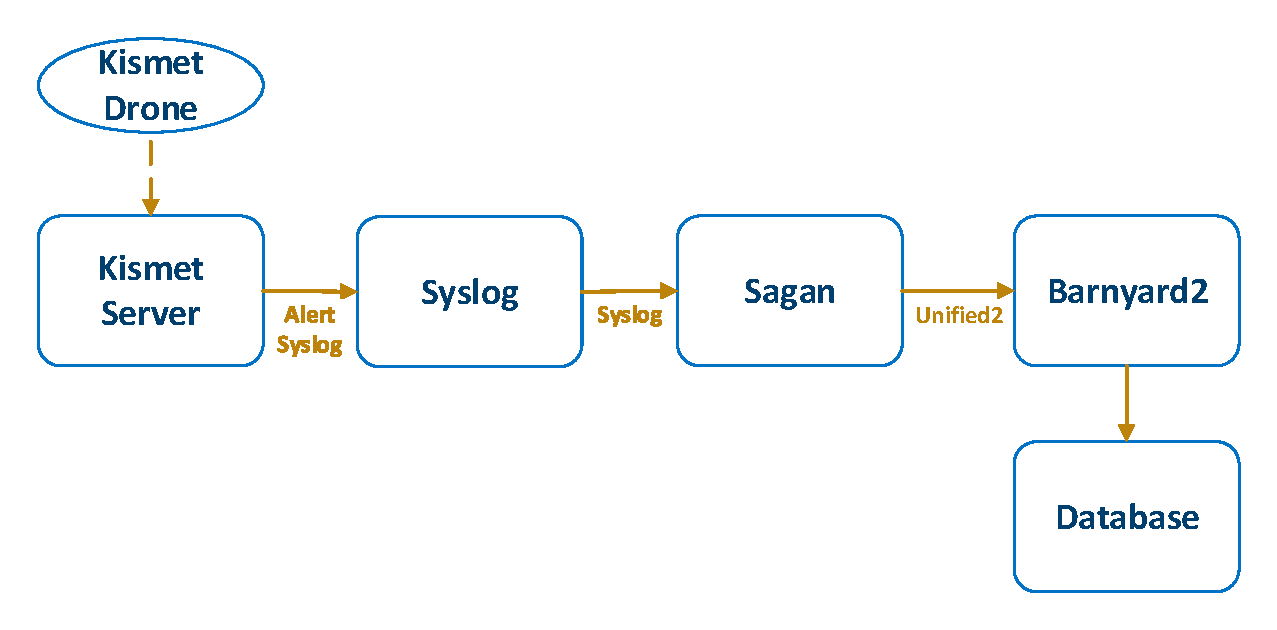
\includegraphics[width=1.0\textwidth]{kismet-workflow}
    \caption{
        \label{fig:kismet-workflow}
        Luồng xử lý dữ liệu của Kismet}
\end{figure}

Sau khi Kismet Drone thu thập các khung quản lý trong phạm vi thu phát sóng, nó sẽ gửi cho Kismet Server. Kismet sử dụng giao thức Kismet Client/Server để liên lạc giữa hai thành phần Kismet Drone và Kismet Server, giao thức này truyền dữ liệu dưới dạng rõ, do vậy thiết lập một kết nối VPN là một việc cần thiết, giúp bảo vệ các dữ liệu này tránh bị những thay đổi không mong muốn. Kismet Server nhận được dữ liệu từ Kismet Drone, sẽ tiến hành xử lý và xuất cảnh báo khi phát hiện tấn công ra các tập tin nhật ký theo mặc định. Vì vậy, đồ án sẽ cài đặt thêm phần mở rộng Alert-Syslog, để Kismet Server có thể gửi các cảnh báo ra cho tiến trình Syslog. Dữ liệu cảnh báo của Kismet và Snort có cú pháp không thống nhất với nhau, trong khi đó, Snort có thể xuất ra định dạng dữ liệu unified2~\cite{snort2017documents}, một định dạng khá phổ biến và được coi như một chuẩn định dạng dữ liệu trong phân tích sự kiện. Do vậy, giải pháp đề ra là cho dữ liệu syslog đi qua phần mềm Sagan, đầu ra của nó sẽ là định dạng unified2 như yêu cầu. Cuối cùng, Barnyard2 sẽ đọc tuần tự các tập tin unified2, để đưa dữ liệu vào cơ sở dữ liệu MySQL một cách hợp lý.

\subsubsection{Luồng xử lý dữ liệu của Snort}
Tiếp đến đồ án sẽ trình bày về luồng xử lý dữ liệu của Snort. Luồng xử lý dữ liệu của Snort được mô tả như Hình~\ref{fig:snort-workflow}.

\begin{figure}[H]
    \centering
    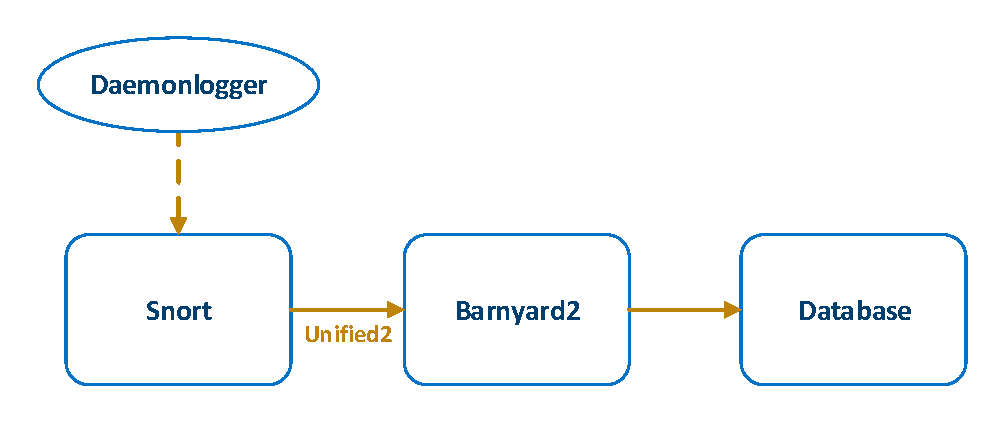
\includegraphics[width=0.9\textwidth]{snort-workflow}
    \caption{
        \label{fig:snort-workflow}
        Luồng xử lý dữ liệu của Snort}
\end{figure}

%\newgeometry{a4paper,left=3.5cm,right=2cm,top=3cm,bottom=3cm}
%\headsep=0pt

Snort cũng như Daemonlogger đều là các phần mềm dựa trên thư viện libpcap. Như đã mô tả về libpcap ở phần trên, Snort sẽ nhận được những gói tin hoàn chỉnh được gửi bởi Daemonlogger thông qua TAP interface. Sau đó, Snort sẽ xử lý những dữ liệu này và xuất các cảnh báo nếu phát hiện các tấn công. Snort hỗ trợ xuất ra định dạng unified2 bằng cách thiết lập tập tin cấu hình cho nó. Dữ liệu unified2 được chuyển đến cho Barnyard2, để phân tích và lưu vào cơ sở dữ liệu.

\subsection{Phần mềm quản lý sự kiện an ninh}
Ngoài ra, để đáp ứng khả năng giám sát và nhận cảnh báo cho người quản trị, hệ thống cũng triển khai một phần mềm quản lý sự kiện an ninh khá đơn giản và hiệu quả, đó là Snorby. Snorby được phát triển trên nền Ruby on Rails, nó sẽ lấy thông tin từ cơ sở dữ liệu MySQL, để đưa ra các thống kê sự kiện và cảnh báo. Snorby cung cấp các chức năng khá trực quan và dễ sử dụng, bao gồm:

\begin{itemize}
\item \emph{Thống kê và báo cáo:} dữ liệu có thể được phân tích và thống kê theo ngày, tuần, tháng, năm. Ngoài ra, nó cũng hỗ trợ xuất báo cáo thành định dạng pdf.
\item \emph{Giám sát và phân loại sự kiện:} các sự kiện được hiển thị theo thời gian thực, người quản trị có thể phân loại những sự kiện này, cũng có thể đưa nó vào hàng đợi để phân loại sau. Snorby cung cấp một số định nghĩa về phân loại có sẵn, hoặc có thể tự định nghĩa theo nhu cầu.
\item \emph{Hiển thị thông tin chi tiết cảnh báo:} Snorby cho phép xem các thông tin chi tiết của một cảnh báo, thậm chí có thể xem chi tiết dữ liệu nguyên thủy bên trong gói tin thu thập được.
\item \emph{Phím tắt:} Snorby sử dụng một hệ thống phím tắt riêng, cho phép người quản trị thay đổi tùy ý. Hệ thống phím tắt này giúp việc phân loại sự kiện hiệu quả và nhanh chóng hơn.
\item \emph{Khả năng mở rộng:} Snorby cũng hỗ trợ một số phần mở rộng từ bên thứ ba.
\end{itemize}

%\restoregeometry

\section{Kết chương}
Như vậy, chương này đồ án đã trình bày về hướng tiếp cận mới của hệ thống KMA-WIDS, cũng như thiết kế tổng quan và chi tiết của nó. Có thể nói, hệ thống WIDS được đề xuất bao gồm đầy đủ các thành phần như một hệ thống IDS tiêu chuẩn như đã trình bày ở chương 2. Chương tiếp theo sẽ trình bày về hiện thực hệ thống, các mô tả cài đặt, giao diện hoạt động, từ đó tiến hành đánh giá về hoạt động của hệ thống.

\chapter{HIỆN THỰC HỆ THỐNG}
\ifpdf
    \graphicspath{{Chapter4/Chapter4Figs/PNG/}{Chapter4/Chapter4Figs/PDF/}{Chapter4/Chapter4Figs/}}
\else
    \graphicspath{{Chapter4/Chapter4Figs/EPS/}{Chapter4/Chapter4Figs/}}
\fi

\section{Mô hình triển khai}
Hệ thống KMA-WIDS có mô hình triển khai như Hình~\ref{fig:diagram-wids-new-demo}, bao gồm:

\begin{itemize}
\item \emph{Access Point \& Sensor:} thiết bị TP-Link TL-WR1043ND.
\item \emph{IDS Server:}  máy tính nhúng Raspberry Pi 2 mẫu B.

\begin{figure}[!htbp]
    \centering
    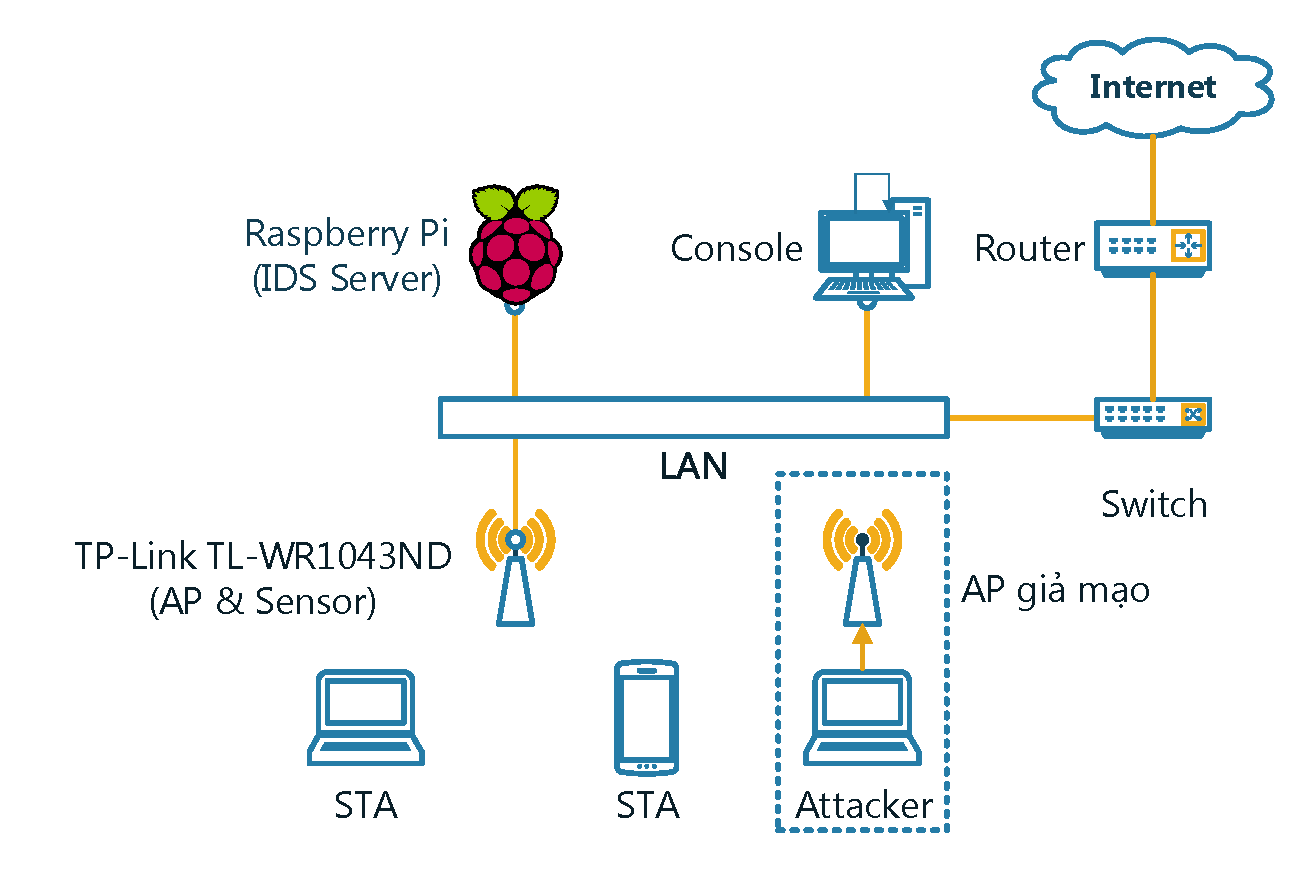
\includegraphics[width=0.9\textwidth]{diagram-wids-new-demo}
    \caption{
        \label{fig:diagram-wids-new-demo}
        Mô hình triển khai hệ thống KMA-WIDS}
\end{figure}

\item \emph{Switch:} một Switch thông thường, kết nối các thành phần của hệ thống WIDS, và kết nối với mạng có dây.
\item \emph{Router:} định tuyến và cung cấp kết nối Internet cho mạng nội bộ.
\item \emph{STA và Attacker:} các máy tính tham gia vào mạng không dây, Attacker sẽ là bên thực hiện các cuộc tấn công. Các STA còn lại là nạn nhân.
\item \emph{Console:} máy tính của quản trị viên, được kết nối vào mạng có dây. Máy tính này sẽ truy cập vào giao diện web Snorby trên IDS Server để giám sát hệ thống và nhận các cảnh báo xâm nhập.
\end{itemize}

\section{Triển khai hệ thống}
\subsection{Xây dựng và cài đặt OpenWrt cho AP}
Sản phẩm TP-Link TL-WR1043ND được đồ án lựa chọn để cài đặt làm AP và Sensor cho hệ thống WIDS. Với dung lượng bộ nhớ flash 8 MB, bộ nhớ RAM 64 MB, việc tự xây dựng một firmware tích hợp sẵn các gói phần mềm Kismet Drone, Daemonlogger và OpenVPN là cần thiết, giúp sử dụng bộ nhớ của thiết bị hiệu quả hơn. Hơn nữa, do các tập tin cấu hình mặc định đã được chỉnh sửa những thay đổi cần thiết, nên firmware sau khi xây dựng là một firmware có tính đóng gói, chỉ cần cài đặt lên thiết bị là có thể sử dụng ngay được.

Để làm được việc này, đầu tiên cần thay thế firmware gốc của nhà sản xuất bằng một firmware OpenWrt được xây dựng sẵn, có thể tải về từ website của dự án OpenWrt~\cite{openwrt2017wiki}. Sau đó thực hiện cài đặt và cấu hình các gói phần mềm thủ công, kiểm tra khả năng chạy thử thành công. Cuối cùng, sao chép các tập tin cấu hình này ra khỏi thiết bị và thực hiện xây dựng lại một firmware tích hợp với các tập tin cấu hình này. Vì không phải phần mềm nào cũng có thể tự khởi chạy khi thiết bị khởi động, nên cần viết thêm một vài script phục vụ công việc này. Firmware mới được tích hợp được cài đặt lại lên thiết bị.

\subsection{Cài đặt các thành phần cho IDS Server}
Do máy tính nhúng Raspberry Pi ban đầu sử dụng một thẻ nhớ trắng, nên cần cài đặt hệ điều hành Raspbian lên. Sau đó, tiến hành cài đặt lần lượt các gói phần mềm OpenVPN, Kismet, Snort, các phần mềm chuyển đổi định dạng dữ liệu là Sagan và Barnyard2, phần mềm giám sát an ninh Snorby và gói phần mềm Apache, MySQL để tạo một HTTP Server và cơ sở dữ liệu phục vụ cho Snorby. Chi tiết phiên bản phần mềm, cũng như các tập luật được trình bày trong phần Phụ lục B.

\section{Kiểm thử hệ thống}
\subsection{Phương pháp và kịch bản}
Hệ thống KMA-WIDS sẽ được kiểm thử bằng hai phương pháp kiểm thử, đầu tiên đó là xác định hệ thống có làm việc được và thực hiện chức năng phát hiện xâm nhập hay không, phương pháp nữa đó là đo thời gian phản hồi của hệ thống trong quá trình phát hiện xâm nhập.

Kịch bản sử dụng đó là thực hiện một số tấn công điển hình từ bên ngoài mạng và từ trong mạng. Kiểm tra khả năng phát hiện tấn công và tạo ra các cảnh báo bằng giao diện web Snorby. Ngoài ra, Kismet và Snort cũng cho phép lưu lại các tập tin pcap, có thể dựa vào đó để tính toán thời gian phản hồi của hệ thống trước các cuộc tấn công.

\subsection{Kiểm thử chức năng}
Kiểm thử chức năng nhằm mục đích kiểm tra việc hệ thống WIDS có làm việc đúng với chức năng của các IDS nói chung. Hệ thống KMA-WIDS này được mong đợi có thể phát hiện các tấn công từ cả bên trong và bên ngoài mạng không dây, và tạo ra các cảnh báo gửi tới giao diện web Snorby. Một số tấn công điển hình sẽ thực hiện đó là:

\begin{itemize}
\item \emph{Tấn công giả mạo AP:} Tấn công này sẽ tạo ra một AP giả mạo với địa chỉ MAC giống như AP hợp pháp, nhằm mục đích lừa cho các STA kết nối vào AP giả mạo.
\item \emph{Tấn công làm lụt khung hủy bỏ xác thực:} Tấn công làm lụt bằng cách liên tục gửi các khung hủy bỏ xác thực tới địa chỉ quảng bá, với địa chỉ MAC nguồn là của AP, làm cho các STA đang kết nối với AP bị ngắt kết nối.
\item \emph{Tấn công quét cổng:} Tấn công quét cổng nhằm dò quét các cổng dịch vụ đang mở trên một STA, nhằm tìm kiếm thông tin về các dịch vụ đang chạy, phục vụ cho các cuộc tấn công khác.
\item \emph{Tấn công khai thác lỗ hỏng bảo mật:} Tấn công khai thác một lỗ hỏng bảo mật bằng cách gửi các payload khai thác lỗ hỏng bảo mật đến STA, từ đó có thể mở một kết nối backdoor và điều khiển máy tính nạn nhân.
\end{itemize}

\subsection{Đo thời gian phản hồi}
Thời gian phản hồi ở đây là thời gian mà hệ thống sử dụng để phát hiện các tấn công và tạo ra cảnh báo. Thời gian phản hồi này có thể được tính toán từ các giá trị khác nhau của thời gian hệ thống cần để phát hiện một tấn công khi nó gửi cảnh báo. Trong tính toán thời gian phản hồi sẽ sử dụng tấn công làm lụt khung hủy bỏ xác thực.

\section{Kết quả kiểm thử}
\subsection{Một số hình ảnh giao diện Snorby}

\begin{figure}[H]
    \centering
    \frame{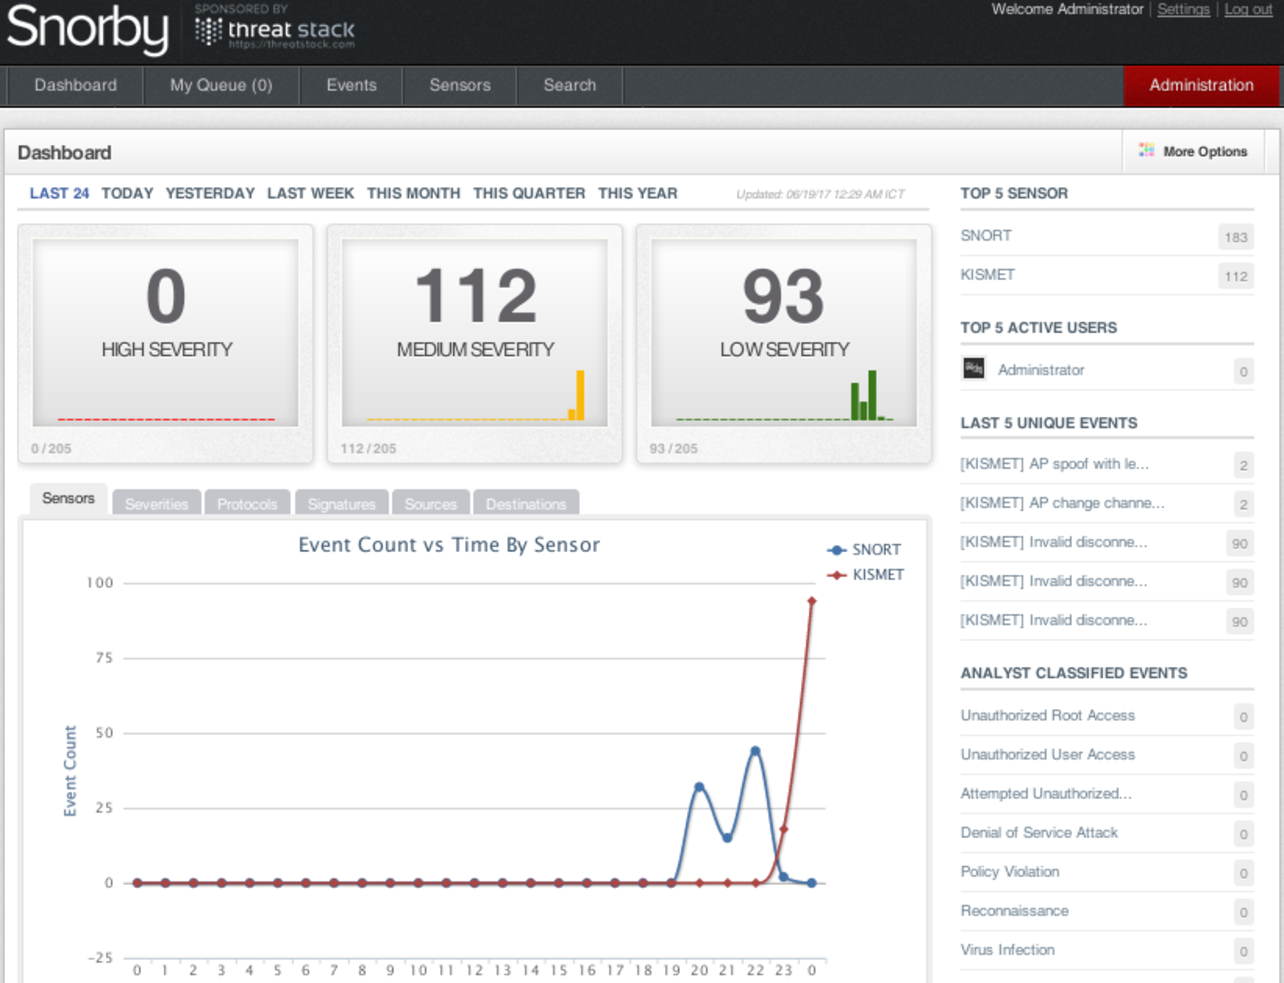
\includegraphics[width=0.95\textwidth]{snorby-dashboard}}
    \caption{
        \label{fig:snorby-dashboard}
        Giao diện bảng điều khiển của Snorby}
\end{figure}

Hình~\ref{fig:snorby-dashboard} là bảng điều khiển của Snorby, tại đây quản trị viên có thể thấy được tổng quan về số lượng sự kiện, mức độ nghiêm trọng, cũng có thể xuất báo cáo thành định dạng pdf.

Hình~\ref{fig:snorby-sensors} là danh sách các Sensor của hệ thống KMA-WIDS, bao gồm một Sensor nhận cảnh báo của Kismet và Sensor còn lại nhận cảnh báo từ Snort.

\begin{figure}[H]
    \centering
    \frame{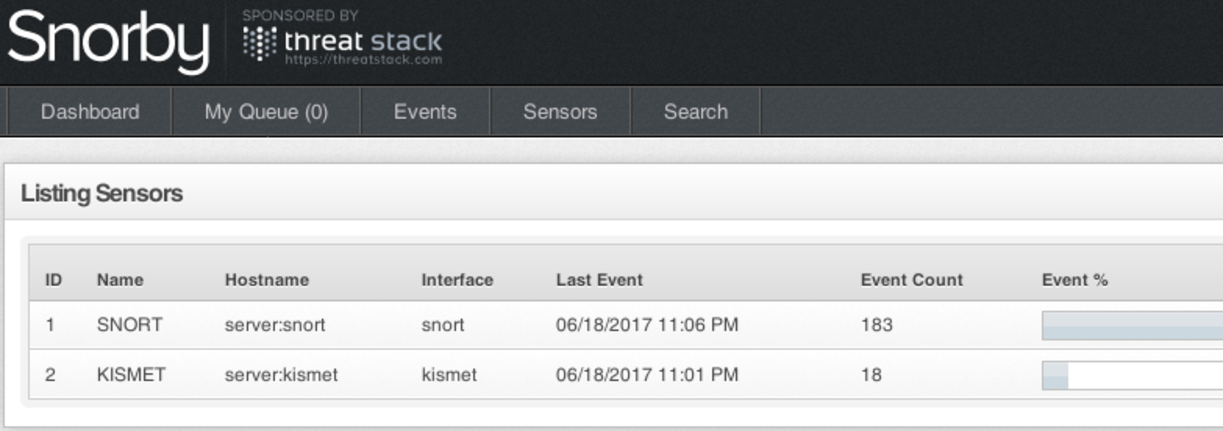
\includegraphics[width=1.0\textwidth]{snorby-sensors}}
    \caption{
        \label{fig:snorby-sensors}
        Danh sách các Sensor trên Snorby}
\end{figure}

Các Hình~\ref{fig:snorby-events} và Hình~\ref{fig:snorby-search} là giao diện quản lý sự kiện và giao diện tìm kiếm của Snorby.

\begin{figure}[H]
    \centering
    \frame{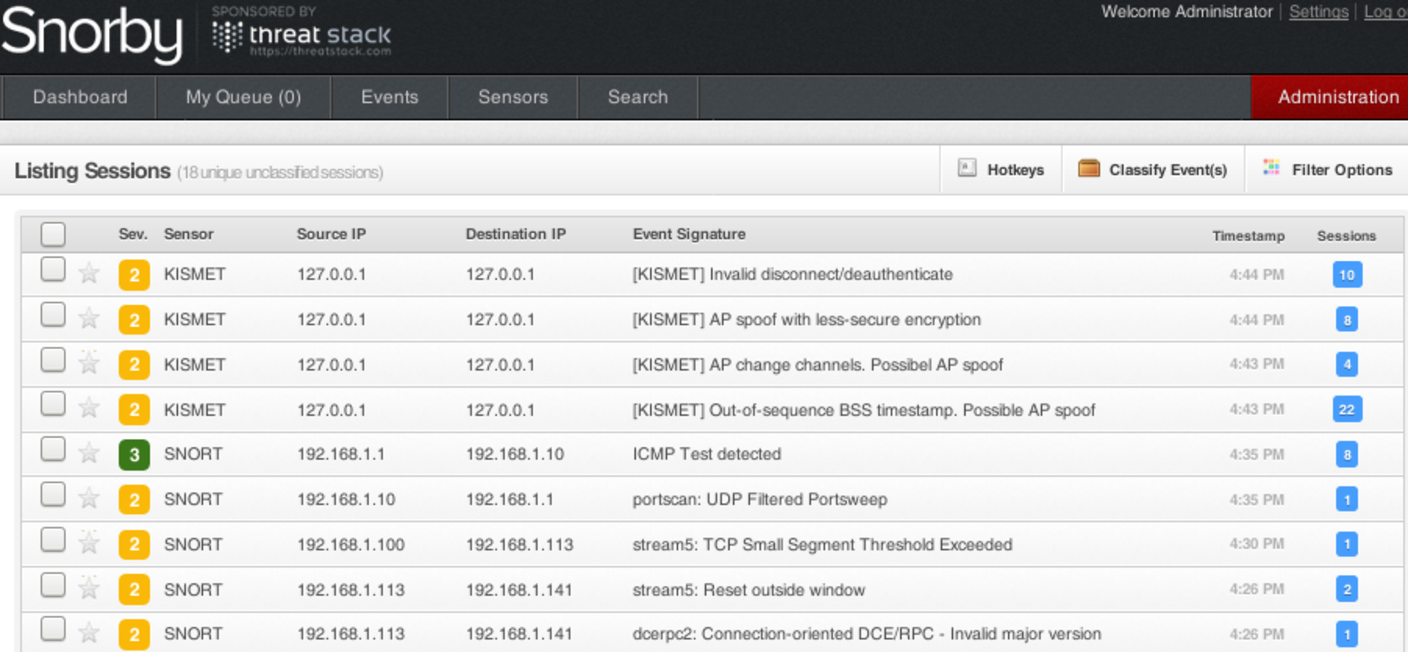
\includegraphics[width=1.0\textwidth]{snorby-events}}
    \caption{
        \label{fig:snorby-events}
        Giao diện quản lý sự kiện của Snorby}
\end{figure}

\begin{figure}[H]
    \centering
    \frame{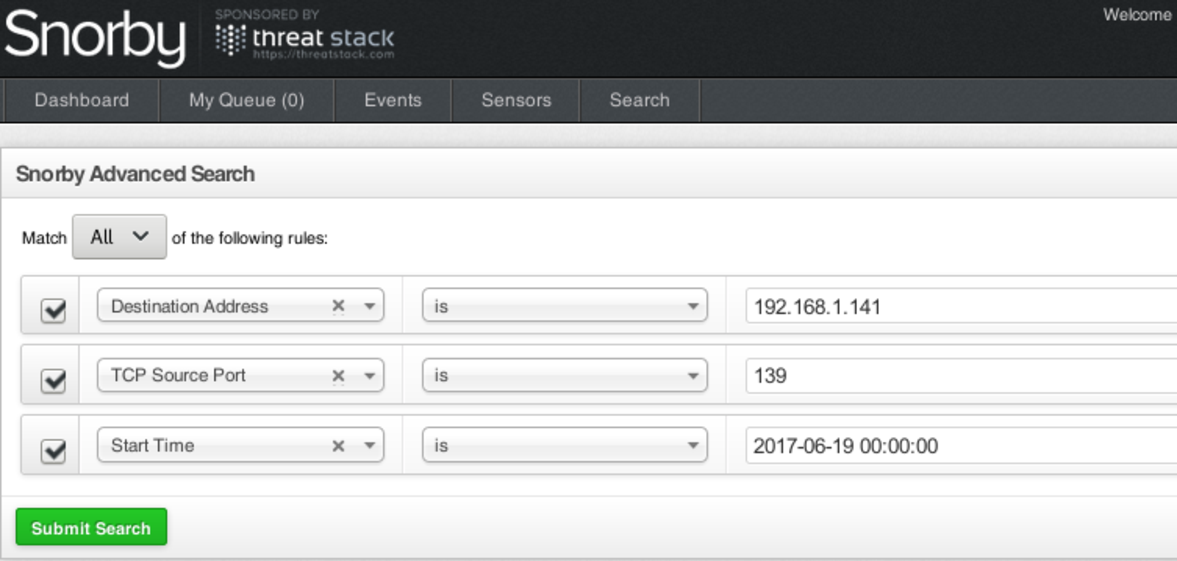
\includegraphics[width=1.0\textwidth]{snorby-search}}
    \caption{
        \label{fig:snorby-search}
        Chức năng tìm kiếm của Snorby}
\end{figure}

\subsection{Kiểm thử chức năng} \label{subsection:kiem-thu-chuc-nang}
\subsubsection*{a) Tấn công giả mạo AP}
Tấn công giả mạo AP sẽ được thực hiện bằng công cụ \emph{airbase-ng}. Công cụ này có thể chuyển đổi một máy tính với card mạng không dây thành một AP. Với một số thiết lập để trông giống AP hợp pháp, khi STA kết nối vào AP giả mạo, toàn bộ lưu lượng truy cập không dây sẽ bị kẻ tấn công chặn bắt và đọc được. Các bước tấn công có thể tóm tắt như sau:

\begin{itemize}
\item \emph{Bước 1:} Kiểm tra trạng thái các card mạng không dây đang hoạt động, chuyển card muốn sử dụng sang chế độ giám sát.
\item \emph{Bước 2:} Dùng công cụ airbase-ng để tạo AP giả mạo với địa chỉ MAC, ESSID và số hiệu kênh giống với AP hợp pháp.
\item \emph{Bước 3:} Cấu hình địa chỉ IP cho giao diện mạng làm AP mà airbase-ng tạo ra.
\item \emph{Bước 4:} Thiết lập định tuyến, NAT để cung cấp kết nối Internet cho AP giả mạo.
\item \emph{Bước 5:} Thiết lập và chạy dịch vụ DHCP để tự động cấp phát khi một STA tham gia vào mạng của AP giả mạo.
\item \emph{Bước 6:} Bật tính năng chuyển tiếp gói tin IP.
\item \emph{Bước 7:} Sử dụng một công cụ phân tích mạng để chặn bắt gói tin, ví dụ tcpdump.
\end{itemize}

Kismet có thể phát hiện được các tấn công giả mạo AP. Cụ thể, Kismet phát hiện tấn công này bằng cách phân tích các nhãn thời gian (timestamp) của các khung báo hiệu được gửi từ AP mà nó giám sát. Các nhãn thời gian có chức năng là để đồng bộ giao dịch giữa STA và AP, có giá trị rất nhỏ và liên tục, do vậy rất khó bị giả mạo. Cảnh báo BSSTIMESTAMP~\cite{mike2016kismet} của Kismet mô tả một nhãn thời gian có số thứ tự không hợp lệ hoặc ngoài phạm vi cho phép có thể cho thấy một tấn công giả mạo AP.

Hình~\ref{fig:bss-timestamp-snorby} là hình ảnh của cảnh báo BSSTIMESTAMP trên giao diện Snorby.

\begin{figure}[H]
    \centering
    \frame{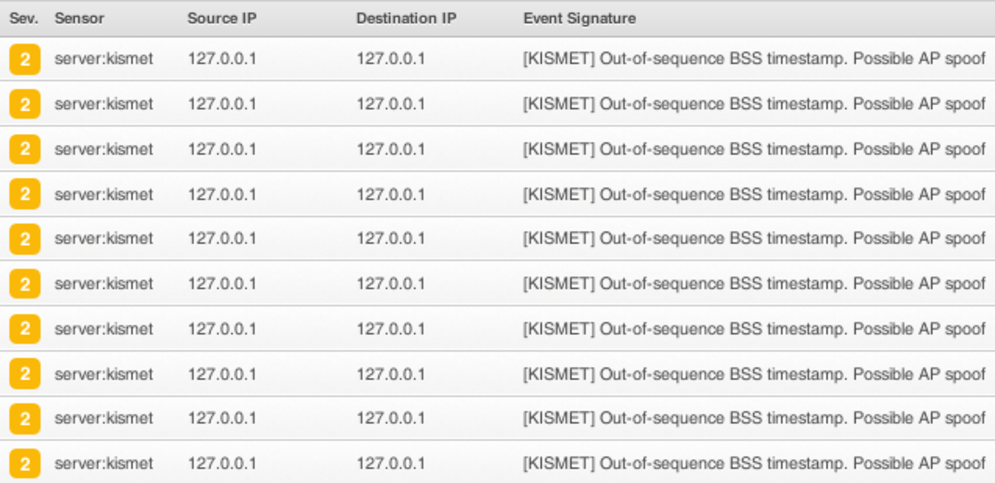
\includegraphics[width=1.0\textwidth]{bss-timestamp-snorby}}
    \caption{
        \label{fig:bss-timestamp-snorby}
        Cảnh báo BSSTIMESTAMP trên Snorby}
\end{figure}

Kismet cũng lưu lại các khung thu thập được vào tập tin định dạng \emph{pcap}, có thể đọc được bằng phần mềm Wireshark. Hình~\ref{fig:bss-timestamp-wireshark} là hình ảnh các khung được đọc bằng phần mềm Wireshark, cho thấy giá trị trường \emph{Timestamp} có thể đọc được dễ dàng.

\begin{figure}[H]
    \centering
    \frame{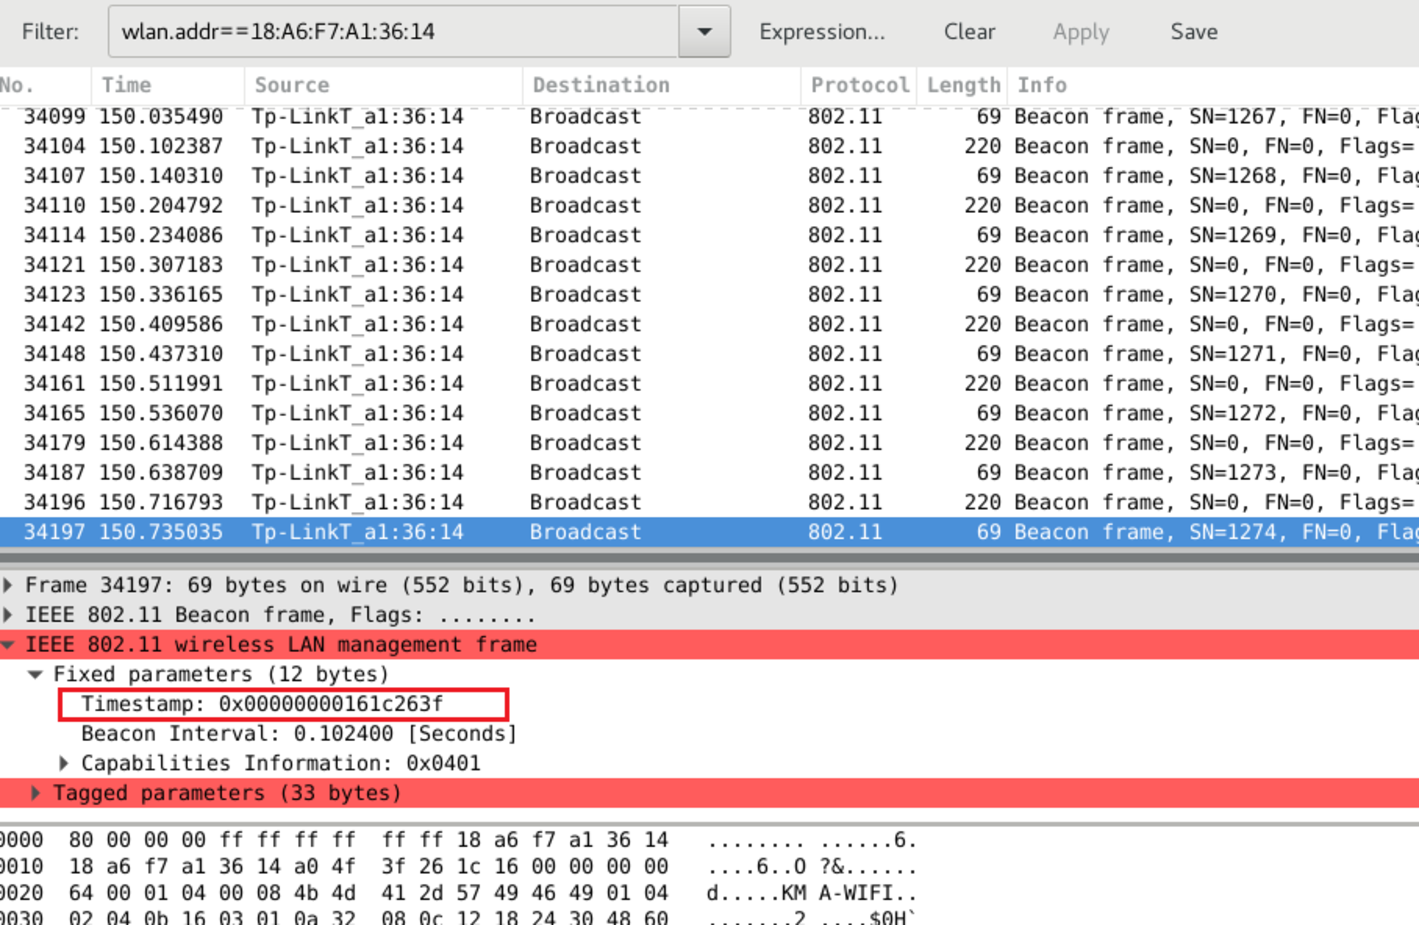
\includegraphics[width=1.0\textwidth]{bss-timestamp-wireshark}}
    \caption{
        \label{fig:bss-timestamp-wireshark}
        Các khung được đọc bằng phần mềm Wireshark}
\end{figure}

\subsubsection*{b) Tấn công làm lụt khung hủy bỏ xác thực}
Công cụ được sử dụng trong tấn công này là \emph{aircrack-ng}. Aircrack-ng là một công cụ đa tính năng, thường được sử dụng để đánh giá hệ thống mạng không dây, ví dụ như tấn công dò khóa WEP, WPA-PSK, tấn công làm lụt khung xác thực và khung hủy bỏ xác thực, thậm chí tấn công tiêm các gói ARP. Trong kiểm thử này sẽ sử dụng tấn công làm lụt bằng các khung hủy bỏ xác thực để ngắt kết nối của tất cả các STA đến AP.  Tấn công này thường được sử dụng để mở đầu một tấn công Man-in-the-middle, nhằm ngắt kết nối các STA với AP hợp pháp làm cho chúng kết nối tới AP giả mạo.

Các câu lệnh đã được sử dụng để tấn công:\\

\begin{lstlisting}
# airmon-ng start wlp3s0
# airodump-ng wlp3s0mon
# aireplay-ng -0 1 -a 18:A6:F7:A1:36:14 -c FF:FF:FF:FF:FF:FF wlp3s0mon
\end{lstlisting}

Trong đó, câu lệnh đầu dùng để bật chế độ giám sát cho giao diện mạng không dây. Tiếp theo là hiển thị các AP trong phạm vi, từ đó xác định được địa chỉ MAC của AP cần tấn công. Cuối cùng là thực hiện gửi các khung hủy bỏ xác thực đến địa chỉ quảng bá.

\begin{figure}[H]
    \centering
    \frame{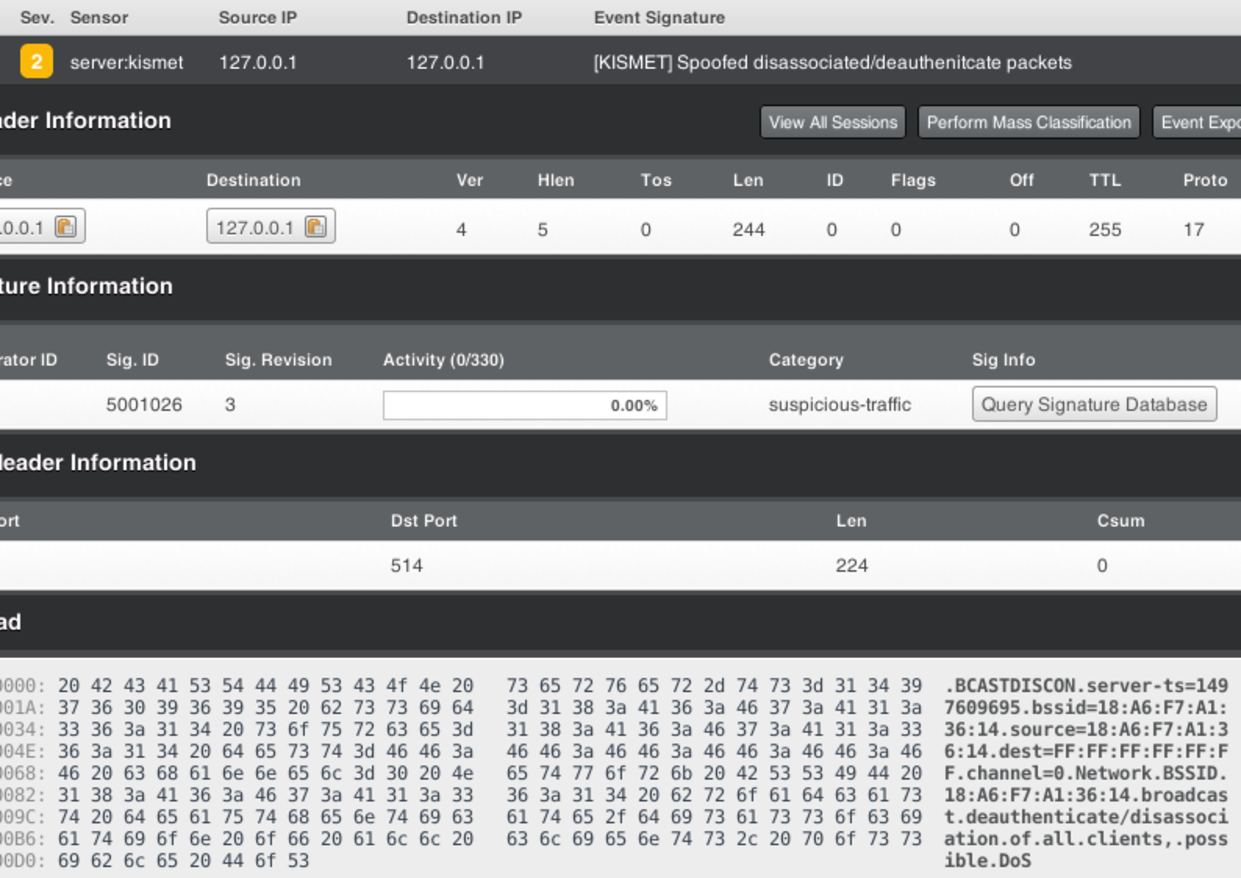
\includegraphics[width=1.0\textwidth]{deauth-snorby}}
    \caption{
        \label{fig:deauth-snorby}
        Chi tiết cảnh báo tấn công làm lụt khung hủy bỏ xác thực}
\end{figure}

Theo tài liệu Kismet~\cite{mike2016kismet}, Kismet hoàn toàn phát hiện được tấn công dạng này. Kết quả kiểm thử cũng cho thấy điều đó. Hình~\ref{fig:deauth-snorby} là chi tiết một cảnh báo tấn công làm lụt khung hủy bỏ xác thực trên Snorby. Ngoài ra, tập tin được Kismet lưu lại cũng dễ dàng quan sát được các khung hủy bỏ xác thực, cụ thể như Hình~\ref{fig:deauth-wireshark}. Trong hình có sử dụng câu lệnh lọc "\emph{wlan.addr==18:A6:F7:A1 :36:14 \&\& wlan.fc.type\_subtype==0x0c}", vế đầu là địa chỉ MAC của AP, vế sau là loại khung, \emph{0x0c} là mã khung phụ của khung quản lý, chính là khung hủy bỏ xác thực đang được xét.

\begin{figure}[H]
    \centering
    \frame{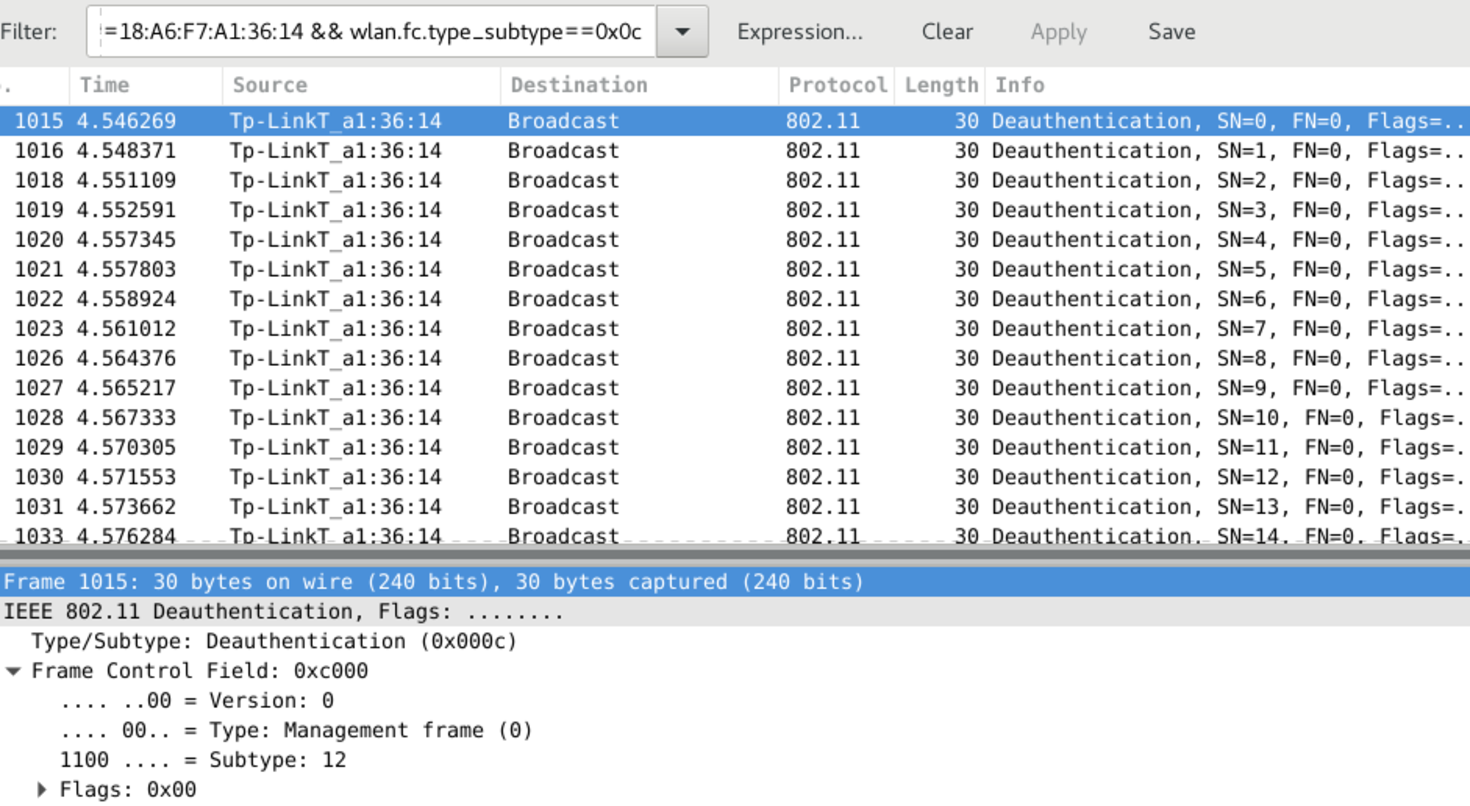
\includegraphics[width=1.0\textwidth]{deauth-wireshark}}
    \caption{
        \label{fig:deauth-wireshark}
        Hình ảnh các khung hủy bỏ xác thực trong Wireshark}
\end{figure}

\subsubsection*{c) Tấn công quét cổng}
Kiểm thử này sử dụng một công cụ quét mạng nổi tiếng, đó là \emph{nmap}. Dưới đây là kết quả của việc quét một máy tính Windows XP, đang tham gia vào mạng không dây. Câu lệnh nmap có ý nghĩa là kiểu quét TCP SYN, quét các cổng từ 1 đến 65535, tùy chọn phát hiện phiên bản của hệ điều hành và dịch vụ được bật. Kiểu quét TCP SYN không thực hiện quá trình bắt tay ba bước hoàn chỉnh, nó chỉ gửi đi gói SYN, sau đó chờ phản hồi. Nếu phản hồi có cờ SYN/ACK được bật, tức là cổng đó đang mở, cờ RST tức là cổng đó đang đóng. Nếu không có phản hồi gì sau một vài lần gửi, hoặc phản hồi chứa mã lỗi ICMP unreachable, cho thấy cổng đó đã được bảo vệ bởi tường lửa~\cite{lyon2009nmap}.\\

\begin{lstlisting}
# nmap -p1-65535 -sV -sS -O 192.168.1.141
Starting Nmap 7.40 ( https://nmap.org ) at 2017-06-19 01:16 +07
Nmap scan report for client.lan (192.168.1.141)
Host is up (0.00031s latency).
Not shown: 65532 closed ports
PORT    STATE SERVICE      VERSION
\end{lstlisting}


\begin{lstlisting}
135/tcp open  msrpc        Microsoft Windows RPC
139/tcp open  netbios-ssn  Microsoft Windows netbios-ssn
445/tcp open  microsoft-ds Microsoft Windows XP microsoft-ds

Device type: general purpose
Running: Microsoft Windows XP
OS CPE: cpe:/o:microsoft:windows_xp::sp2 cpe:/o:microsoft:windows_xp::sp3
OS details: Microsoft Windows XP SP2 or SP3
Network Distance: 1 hop
Service Info: OSs: Windows, Windows XP; CPE: cpe:/o:microsoft:windows, cpe:/o:microsoft:windows_xp
\end{lstlisting}

\begin{figure}[H]
    \centering
    \frame{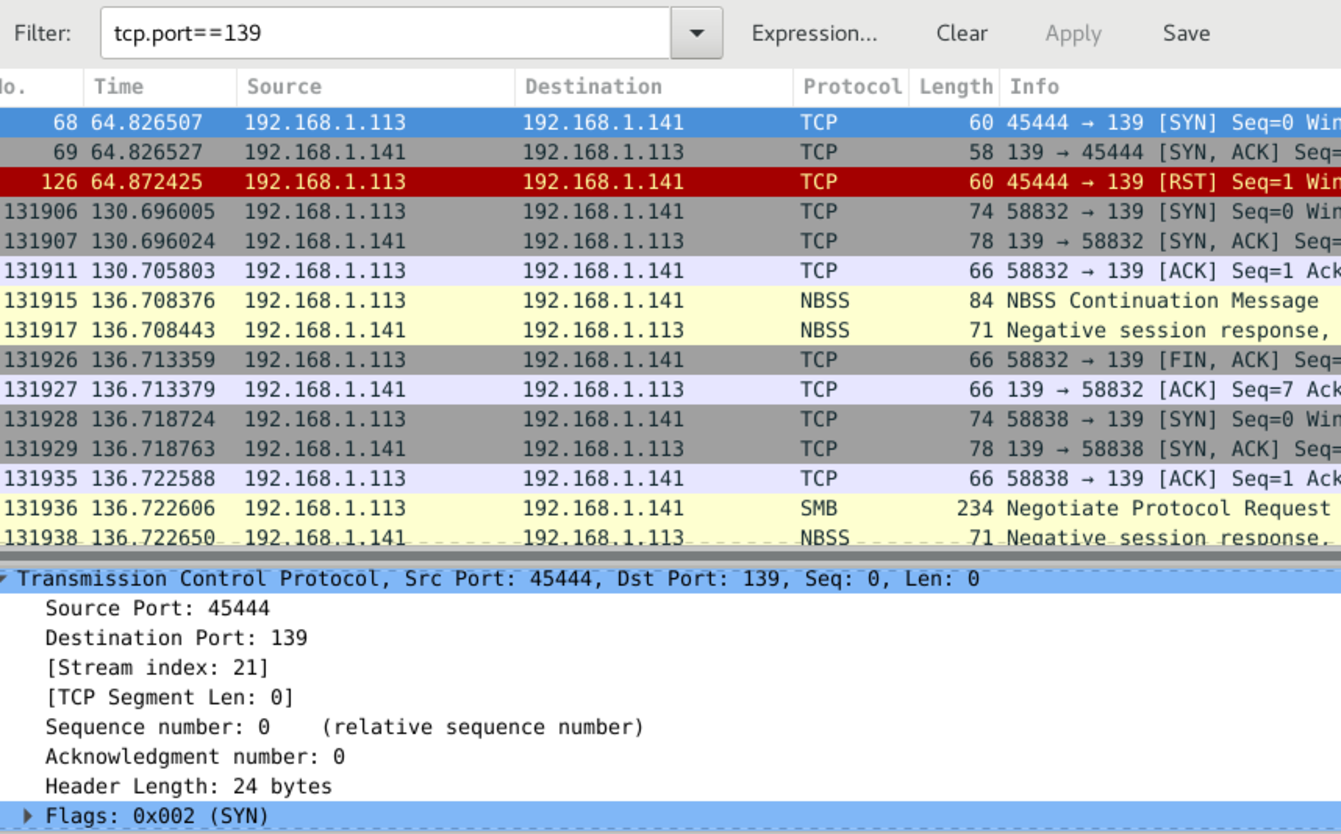
\includegraphics[width=1.0\textwidth]{port-scanning-139}}
    \caption{
        \label{fig:port-scanning-139}
        Các gói tin quét cổng thu thập được}
\end{figure}

Hình~\ref{fig:port-scanning-139} là gói tin pcap được thu thập ở máy nạn nhân. Trong đó, \emph{192.168.1.113} là địa chỉ IP của máy tấn công, \emph{192.168.1.141} là địa chỉ IP của máy nạn nhân. Câu lệnh lọc "\emph{tcp.port==139}" được sử dụng nhằm lọc các gói tin có liên quan đến cổng 139, chính là số hiệu cổng đang mở trên máy nạn nhân. Có thể thấy ngay qua 3 gói tin đầu tiên, trước hết kẻ tấn công mở kết nối TCP đến máy nạn nhân qua cổng 139 bằng gói tin có cờ SYN bật; tiếp đến, máy nạn nhân gửi lại gói tin có cờ SYN/ACK được bật, do đó kẻ tấn công biết được cổng 139 đang mở. Nếu như một quá trình bắt tay ba bước bình thường, máy tấn công sẽ gửi lại gói tin có cờ ACK được bật để thiết lập kết nối, tuy nhiên, nó đã gửi lại gói RST. Xét tiếp các gói tin phía sau, do kẻ tấn công muốn biết rõ dịch vụ đang chạy qua cổng 139 là dịch vụ gì, nên nó đã thiết lập quá trình bắt tay ba bước đầy đủ, để kết nối với máy nạn nhân, quá đó biết được dịch vụ cụ thể là gì.

Tấn công này được phát hiện bằng Snort. Cảnh báo được gửi tới Snorby như Hình~\ref{fig:port-scanning-attack-snorby}.

\begin{figure}[H]
    \centering
    \frame{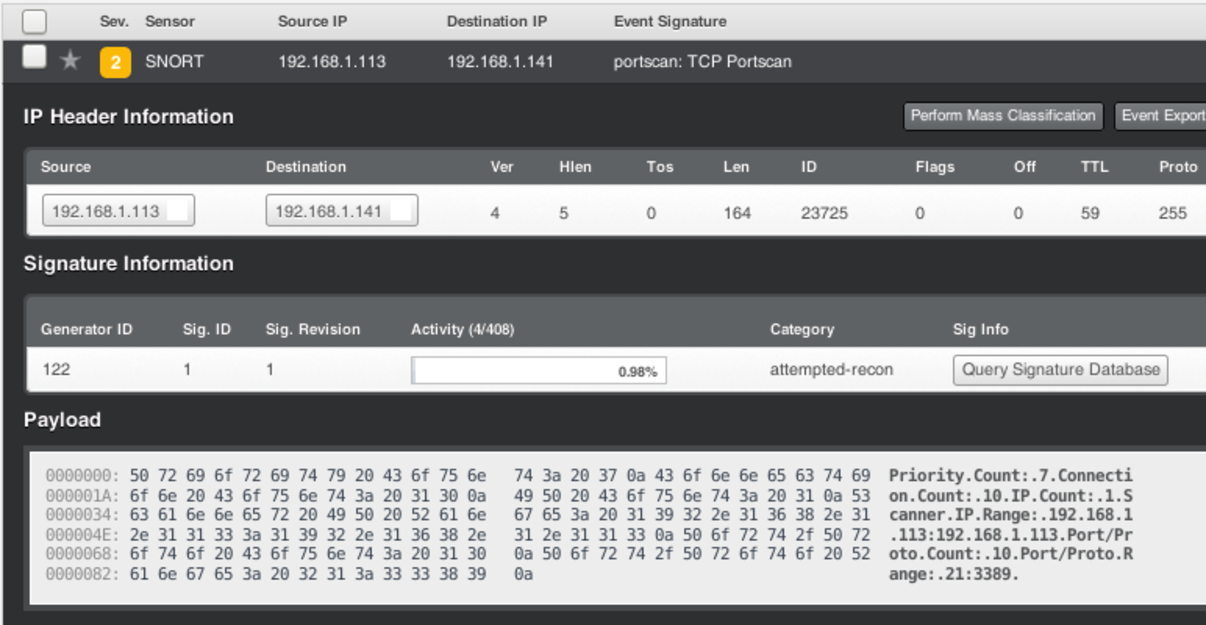
\includegraphics[width=1.0\textwidth]{port-scanning-attack-snorby}}
    \caption{
        \label{fig:port-scanning-attack-snorby}
        Cảnh báo tấn công quét cổng trên Snorby}
\end{figure}

\subsubsection*{d) Khai thác lỗ hỏng bảo mật MS08-067}
MS08-067 là một lỗ hỏng điển hình trên hệ điều hành Windows, cho phép kẻ tấn công thực thi mã lệnh từ xa. Cụ thể, giao thức RPC của dịch vụ Server Service trong Windows hỗ trợ một thủ tục được gọi từ xa và xử lý các yêu cầu đổi đường dẫn (ví dụ, \emph{{\textbackslash \textbackslash}C{\textbackslash}Program Files{\textbackslash}..{\textbackslash}Windows}) về định dạng đường dẫn Canonicalization ngắn gọn hơn (\emph{{\textbackslash \textbackslash}C{\textbackslash}Windows}). Tuy nhiên, với một đường dẫn quá dài, Windows xử lý không tốt dẫn đến lỗ hỏng tràn bộ đệm~\cite{microsoft2008ms08067}. Bằng cách chuyển hướng lỗ hỏng tràn bộ đệm, kẻ tấn công có thể tiêm vào các mã lệnh và thực thi từ xa theo ý mình.

Tấn công này được thực hiện sử dụng công cụ Metasploit, tóm tắt các câu lệnh tấn công như sau:\\

\begin{lstlisting}
msf > use exploit/windows/smb/ms08_067_netapi
msf exploit(ms08_067_netapi) > show targets
            ...targets...
msf exploit(ms08_067_netapi) > set TARGET <target-id>
msf exploit(ms08_067_netapi) > show options
            ...show...
msf exploit(ms08_067_netapi) > set RHOST <ip-address>
msf exploit(ms08_067_netapi) > exploit
\end{lstlisting}

\begin{figure}[H]
    \centering
    \frame{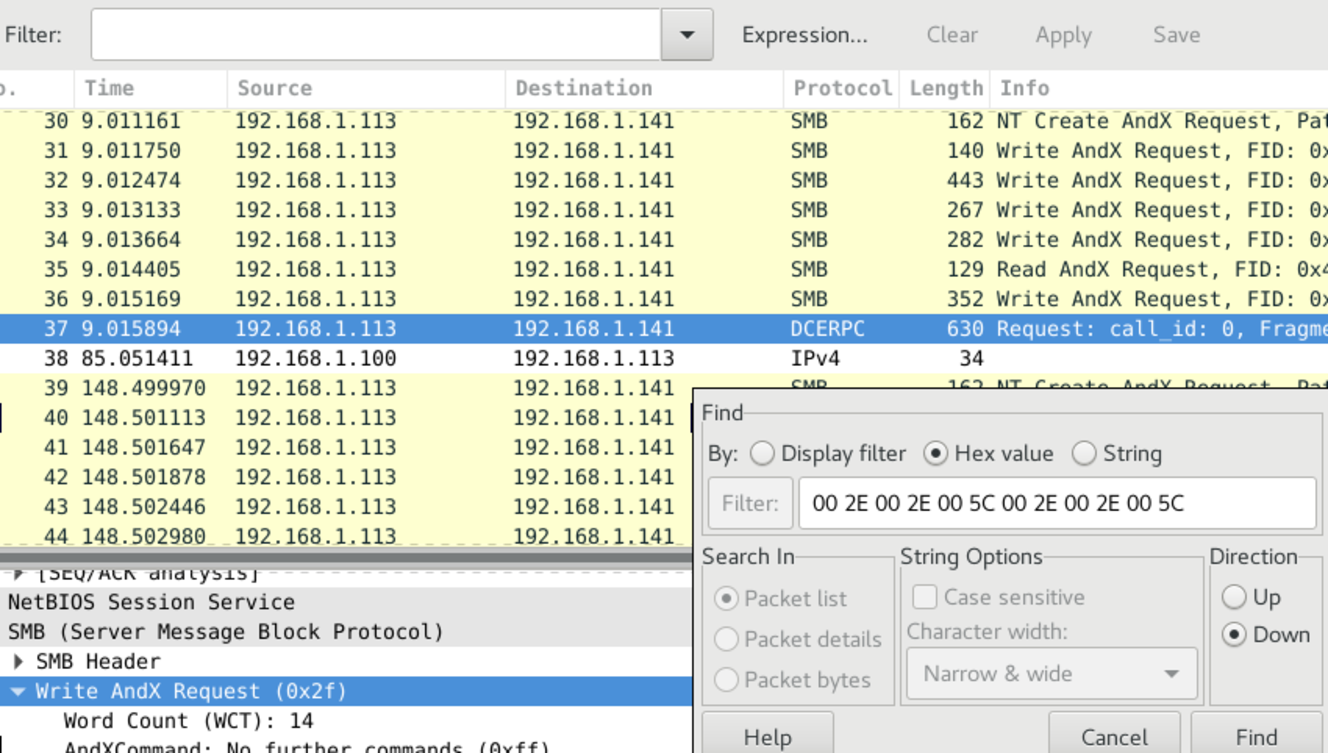
\includegraphics[width=1.0\textwidth]{ms08-067-snort-wireshark}}
    \caption{
        \label{fig:ms08-067-snort-wireshark}
        Các gói tin từ tấn công khai thác lỗ hỏng MS08-067}
\end{figure}

Hình~\ref{fig:ms08-067-snort-wireshark} là hình ảnh các gói tin mà Snort lưu lại. Trong phần tìm kiếm là các byte lấy từ luật mà Snort dùng để phát hiện tấn công này, hoàn toàn khớp với dữ liệu thu thập được. Với việc cấu hình luật phù hợp, Snort có thể phát hiện tấn công này và đưa ra cảnh báo tới giao diện Snorby như Hình~\ref{fig:ms08-067-snort-snorby}. Tấn công này được phân loại mức nghiêm trọng là 1, cao nhất trong ba mức nghiêm trọng của Snorby.

\begin{figure}[H]
    \centering
    \frame{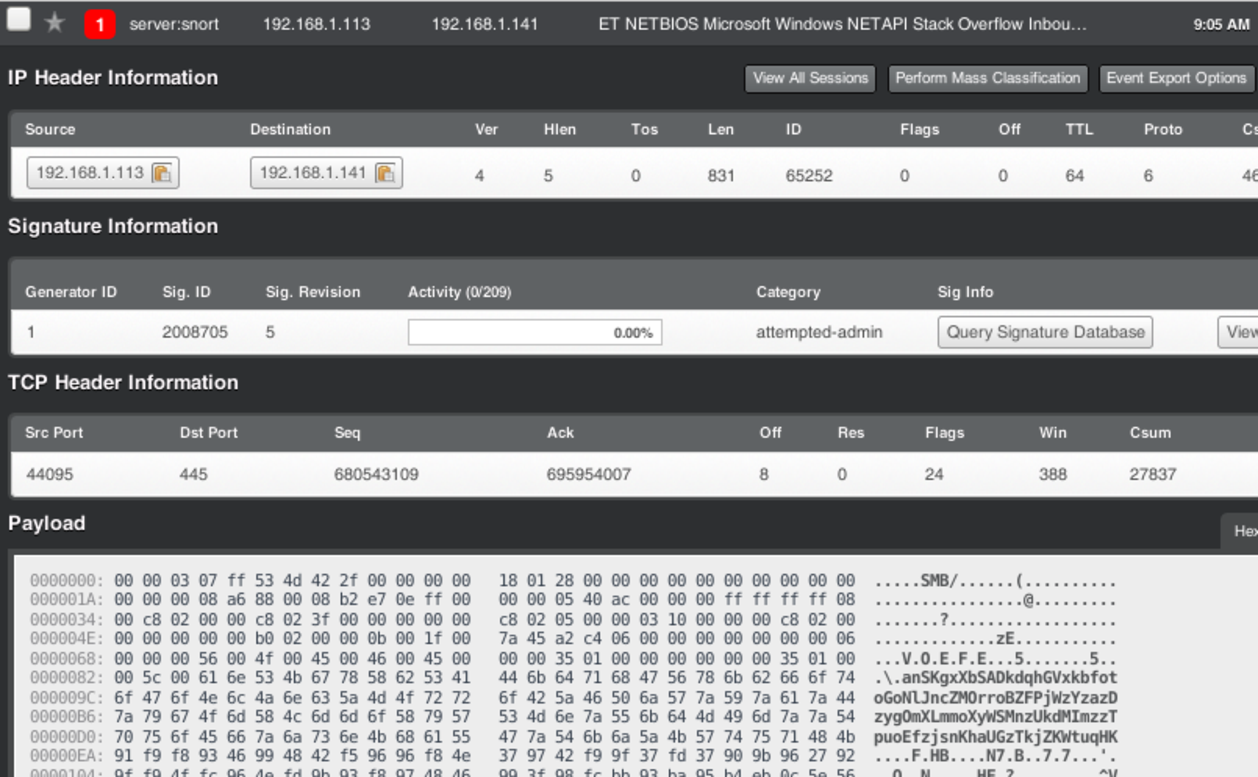
\includegraphics[width=1.0\textwidth]{ms08-067-snort-snorby}}
    \caption{
        \label{fig:ms08-067-snort-snorby}
        Cảnh báo tấn công khai thác lỗ hỏng MS08-067 trên Snorby}
\end{figure}

\subsection{Đo thời gian phản hồi}
Để đo thời gian phản hồi, đồ án tập trung vào tấn công làm lụt khung hủy bỏ xác thực. Tấn công này gửi liên tục nhiều khung hủy bỏ xác thực, do đó có thể đo được thời gian, số lượng khung, cũng như số lượng cảnh báo. Số liệu phân tích được lấy từ tập tin pcap trong phần kiểm thử chức năng.

Thời gian phản hồi được tính toán từ các thời gian khác nhau từ khi tấn công gửi đi khung hủy bỏ xác thực cho đến khi tấn công được phát hiện bởi Kismet. Các trường giá trị thời gian trong tập tin pcap có thể đọc được bằng phần mềm Wireshark như Hình~\ref{fig:deauth-attack-detect}.

\begin{figure}[H]
    \centering
    \frame{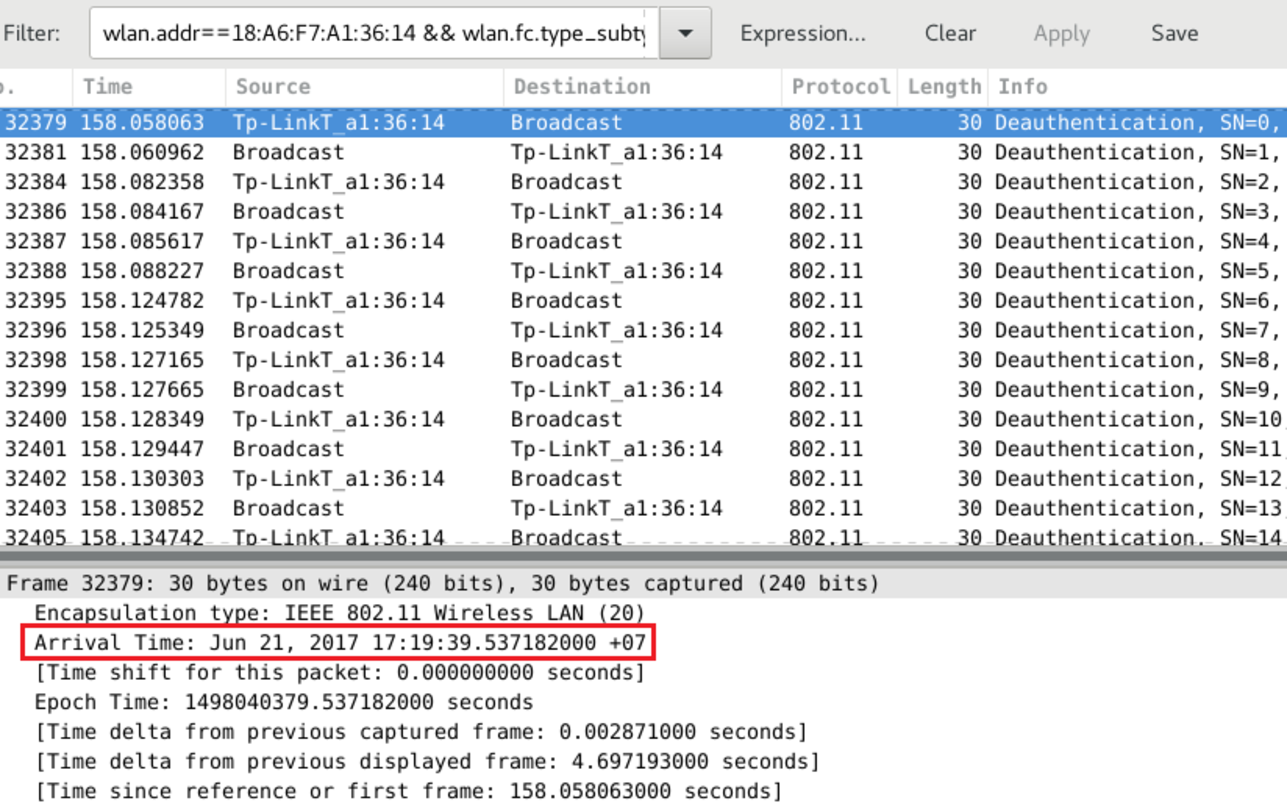
\includegraphics[width=1.0\textwidth]{deauth-attack-detect}}
    \caption{
        \label{fig:deauth-attack-detect}
        Thời gian bắt đầu phát hiện khung đầu tiên}
\end{figure}

Hình trên cho thấy, Kismet phát hiện khung hủy bỏ xác thực đầu tiên nhận được từ kẻ tấn công có \emph{Sequence Number (SN) = 0} vào thời gian \emph{Jun 21, 2017 17:19:39.537182000 +07}. Mỗi khung có một Sequence Number duy nhất, giá trị này sẽ được tăng lên khi một STA gửi cùng một khung giống với khung trước đó. Giá trị lớn nhất của SN là 4096. Sau khi đạt giá trị lớn nhất, số SN sẽ bắt đầu lại từ 0~\cite{guo2005sequence}.

Để đo được thời gian phản hồi của hệ thống WIDS, về phía kẻ tấn công cũng đã chạy Kismet để tự thu thập lại các khung nhằm xác định thời gian gửi đi. Hình~\ref{fig:deauth-attack-detect} là thông tin thời gian gửi của khung đầu tiên mà máy tấn công thu thập được.

Kẻ tấn công gửi khung hủy bỏ xác thực đầu tiên \emph{SN = 0} vào thời gian \emph{Jun 21, 2017 17:19:39.534660000 +07}. Sự khác nhau về thời gian từ khi khung tấn công được gửi tới khi Kismet của hệ thống WIDS phát hiện được là chậm hơn \emph{0.002522000} giây. Bảng~\ref{tab:response-time-table} là số liệu thống kê trong 10 khung đầu tiên.

\begin{figure}[H]
    \centering
    \frame{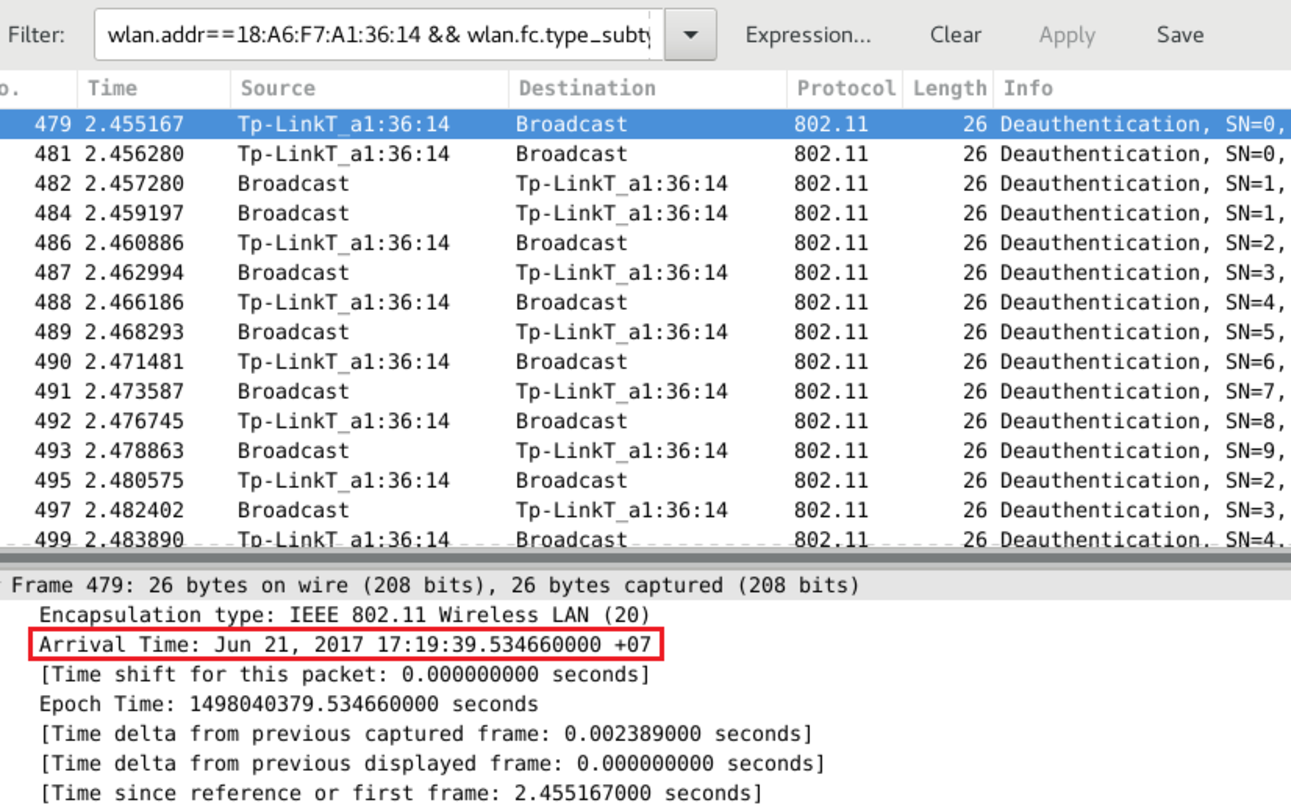
\includegraphics[width=1.0\textwidth]{deauth-attack-sent}}
    \caption{
        \label{fig:deauth-attack-sent}
        Thời gian bắt đầu gửi khung đầu tiên}
\end{figure}

\begin{table}[H]
\centering
\small
\setlength{\extrarowheight}{1pt}
\caption{\label{tab:response-time-table}Thống kê thời gian phản hồi trong 10 khung đầu tiên}
\begin{tabular}{|c|c|c|c|}
\hline
\textbf{SN} & \textbf{Thời gian gửi} & \textbf{Kismet phát hiện} & \textbf{Thời gian phản hồi} \\ \hline
0           & 17:19:39.534660000     & 17:19:39.537182000        & 0.002522000                 \\ \hline
1           & 17:19:39.536773000     & 17:19:39.540081000        & 0.003308000                 \\ \hline
2           & 17:19:39.540379000     & 17:19:39.561477000        & 0.021098000                 \\ \hline
3           & 17:19:39.542487000     & 17:19:39.563286000        & 0.020799000                 \\ \hline
4           & 17:19:39.545679000     & 17:19:39.564736000        & 0.019057000                 \\ \hline
5           & 17:19:39.547786000     & 17:19:39.567346000        & 0.019560000                 \\ \hline
6           & 17:19:39.550974000     & 17:19:39.603901000        & 0.052927000                 \\ \hline
7           & 17:19:39.553080000     & 17:19:39.604468000        & 0.051388000                 \\ \hline
8           & 17:19:39.556238000     & 17:19:39.606284000        & 0.050046000                 \\ \hline
9           & 17:19:39.558356000     & 17:19:39.606784000        & 0.048428000                 \\ \hline
\multicolumn{3}{|c|}{\textbf{Trung bình}}                        & \textbf{0.028913300}        \\ \hline
\end{tabular}
\end{table}

Vậy thời gian phản hồi trung bình cho các tấn công đầu tiên là \emph{0.028913300} giây. Với việc kiểm thử thời gian phản hồi, cho thấy hệ thống KMA-WIDS có khả năng phản hồi gần như lập tức trước các tấn công. Tuy nhiên, do thiết bị AP cũng đồng thời là WIDS Sensor, nên tấn công làm lụt khung hủy bỏ xác thực đang trực tiếp tấn công lên WIDS Sensor, dẫn đến thời gian phản hồi có xu hướng tăng theo thời gian, tức là hiệu suất của WIDS Sensor bị giảm.

\section{Tổng kết và đánh giá hệ thống}
Như vậy, qua bốn chương đã trình bày, đồ án đã nghiên cứu và triển khai thành công hệ thống KMA-WIDS với các chức năng chính: giám sát và phát hiện các tấn công từ bên trong và bên ngoài mạng WiFi, đưa ra các cảnh báo kịp thời thông qua giao diện quản trị. Khả năng phát hiện các tấn công bên ngoài mạng của hệ thống không kém gì so với một giải pháp dành cho doanh nghiệp.

Về các tấn công bên trong mạng WiFi, chúng cũng đa dạng và tương tự như các tấn công bên trong mạng có dây. Đồ án chỉ kiểm thử khả năng phát hiện một số tấn công điển hình, cấu hình luật phù hợp để Snort có thể phát hiện và tạo ra các cảnh báo. Qua đó thấy được, hệ thống WIDS đề xuất hoàn toàn có khả năng phát hiện các tấn công bên trong mạng WiFi.

Sau đây là tóm tắt các ưu điểm nổi bật của hệ thống KMA-WIDS:

\begin{itemize}
\item Hệ thống KMA-WIDS được tích hợp lên thiết bị Access Point thông thường, và máy tính nhúng Raspberry Pi, mang lại sự phù hợp về hiệu quả và chi phí.
\item Hệ thống có khả năng phát hiện được cả tấn công từ bên trong và bên ngoài mạng WiFi, bảo vệ hạ tầng mạng WiFi và người dùng khỏi các mối đe dọa bảo mật.
\item Hệ thống cũng cung cấp giao diện quản trị Snorby trực quan và dễ sử dụng.
\item Bằng việc ứng dụng các phần mềm mã nguồn mở, hệ thống có khả năng mở rộng cao, các phần mềm mã nguồn mở này vẫn đang được cộng đồng phát triển từng ngày.
\item Hệ thống sử dụng các bản phân phối dựa trên Linux, nên có thể tương thích với hầu hết các loại phần cứng phổ biến.\\
\end{itemize}

Bên cạnh đó, vì thời gian nghiên cứu còn hạn chế, hệ thống KMA-WIDS vẫn còn tồn tại một số vấn đề cần quan tâm như:

\begin{itemize}
\item Hệ thống hiện chỉ hỗ trợ phát hiện các tấn công, chưa có biện pháp để ngăn chặn các tấn công khi chúng xảy ra.
\item Khả năng phát hiện tấn công bên ngoài phụ thuộc hoàn toàn vào Kismet, không hỗ trợ viết luật để nhận diện tấn công mới. Snort cần được cấu hình tập luật phù hợp, để có thể phát hiện các tấn công bên trong mạng.
\item Hiệu năng của hệ thống cần được tối ưu hơn nữa để có thể triển khai rộng rãi trong thực tế. Công việc này đòi hỏi quá trình nghiên cứu và phát triển để làm cho các phần mềm thực sự hoạt động hiệu quả trên thiết bị nhúng.\\
\end{itemize}

Những vấn đề này sẽ được đề cập rõ hơn trong phần~\ref{section:huong-phat-trien} - Hướng phát triển của hệ thống trong chương tiếp theo.


%\def\baselinestretch{1.3}
\chapter{KẾT LUẬN VÀ HƯỚNG PHÁT TRIỂN}
\ifpdf
    \graphicspath{{Conclusions/ConclusionsFigs/PNG/}{Conclusions/ConclusionsFigs/PDF/}{Conclusions/ConclusionsFigs/}}
\else
    \graphicspath{{Conclusions/ConclusionsFigs/EPS/}{Conclusions/ConclusionsFigs/}}
\fi

%\def\baselinestretch{1.66}
\renewcommand{\baselinestretch}{1.3}

\section{Kết luận}
Đồ án đã đạt được những kết quả sau:

\begin{itemize}
\item Tiếp cận với các thiết bị nhúng, cũng như ứng dụng các thiết bị này vào nghiên cứu xây dựng các giải pháp bảo mật.
\item Hệ thống lại các kiến thức cơ sở về hoạt động của mạng WiFi, các tấn công xảy ra trong mạng WiFi.
\item Đồ án tập trung nghiên cứu về hệ thống phát hiện xâm nhập, các phương pháp phát hiện xâm nhập phổ biến. Sau đó nghiên cứu những đặc điểm riêng của phát hiện xâm nhập mạng WiFi.
\item Thêm nữa, đồ án cũng thực hiện khảo sát về các hệ thống đã được phát triển, để thấy được ưu nhược điểm của chúng.
\item Từ những kết quả nghiên cứu và tìm hiểu, đồ án đã đề xuất và hiện thực thành công một hệ thống WIDS có tên là KMA-WIDS, để giám sát và phát hiện các tấn công từ bên ngoài và bên trong mạng WiFi.
\end{itemize}

\section{Hướng phát triển} \label{section:huong-phat-trien}

Từ những kết quả đạt được, đồ án hy vọng sẽ mở ra một hướng nghiên cứu tiềm năng về tích hợp bảo mật trên thiết bị nhúng, cụ thể là giải pháp phát hiện xâm nhập mạng WiFi. Vì vậy, để hệ thống có thể được ứng dụng rộng rãi trong thực tế, đồ án có một số hướng phát triển đó là:

\begin{itemize}
\item Nghiên cứu mã nguồn của các phần mềm phát hiện xâm nhập được sử dụng, để từ đó có thể phát triển thêm, tối ưu vấn đề sử dụng tài nguyên để hệ thống đạt hiệu năng cao hơn trên thiết bị nhúng.
\item Phát triển thêm các phần mở rộng cho các phần mềm mà hệ thống sử dụng, để khai thác các tính năng bổ sung, cũng như đóng góp vào cộng đồng mã nguồn mở.
\item Phát triển thêm tính năng cảnh báo theo thời gian thực qua SMS hoặc ứng dụng \emph{bot}. Ứng dụng bot là một chương trình tự động gửi tin nhắn nhanh đến người dùng, có rất nhiều bot miễn phí như facebook, telegram,~\ldots
\item Nghiên cứu tính năng ngăn chặn xâm nhập của Snort để áp dụng vào hệ thống WIDS nhằm ngăn chặn các tấn công bên trong mạng WiFi.
\item Xây dựng bộ tài liệu hướng dẫn triển khai, cũng như hướng dẫn sử dụng trực quan và đầy đủ, giúp người dùng tiếp cận và sử dụng hệ thống.
\end{itemize}



%%% ----------------------------------------------------------------------

% ------------------------------------------------------------------------

%%% Local Variables: 
%%% mode: latex
%%% TeX-master: "../thesis"
%%% End: 


\backmatter  

%% ********************************** Bibliography ******************************
%\begin{spacing}{0.9}
%
%% To use the conventional natbib style referencing
%% Bibliography style previews: http://nodonn.tipido.net/bibstyle.php
%% Reference styles: http://sites.stat.psu.edu/~surajit/present/bib.htm
%
%\bibliographystyle{apalike}
%%\bibliographystyle{unsrt} % Use for unsorted references  
%%\bibliographystyle{plainnat} % use this to have URLs listed in References
%\cleardoublepage
%\bibliography{References/references} % Path to your References.bib file
%
%
%% If you would like to use BibLaTeX for your references, pass `custombib' as
%% an option in the document class. The location of 'reference.bib' should be
%% specified in the preamble.tex file in the custombib section.
%% Comment out the lines related to natbib above and uncomment the following line.
%
%%\printbibliography[heading=bibintoc, title={References}]
%
%
%\end{spacing}

\bibliographystyle{apalike} %
%\bibliographystyle{plainnat} %
%\bibliographystyle{Classes/CUEDbiblio.bst} %
%\bibliographystyle{Classes/jmb} % bibliography style
\renewcommand{\bibname}{TÀI LIỆU THAM KHẢO} % changes default name Bibliography to References
\bibliography{References/references} % Path to your References.bib file

\appendix
\chapter*{PHỤ LỤC A: THÔNG TIN TÁC GIẢ}
\addcontentsline{toc}{chapter}{PHỤ LỤC A}

\renewcommand{\baselinestretch}{1.5}
\section*{Thông tin giảng viên hướng dẫn}

\noindent \textbf{TS. Nguyễn Anh Tuấn}\\
\noindent Khoa Mạng Máy tính và Truyền thông\\
\noindent Trường Đại học Công nghệ Thông tin - Đại học Quốc gia TP. Hồ Chí Minh\\
\noindent Km20 Xa lộ Hà Nội, Linh Trung, Thủ Đức, TP.Hồ Chí Minh\\
\noindent Điện thoại: (+84) 932 215 030\\
\noindent Email: tuanna@uit.edu.vn\\
\noindent Website: uit.edu.vn/\textasciitilde tuanna\\

\section*{Thông tin sinh viên thực hiện}

\noindent \textbf{Hà Văn Toàn}\\
\noindent Lớp: AT9D - Học viện Kỹ thuật Mật mã\\
\noindent 17A Cộng Hòa, P.4, Q.Tân Bình, TP.Hồ Chí Minh\\
\noindent Điện thoại: (+84) 946 234 768\\
\noindent Email: toanhv.vietnam@gmail.com\\


\chapter*{PHỤ LỤC B: THÔNG TIN PHẦN MỀM SỬ DỤNG}
\addcontentsline{toc}{chapter}{PHỤ LỤC B}

\renewcommand{\baselinestretch}{1.3}
\begin{itemize}
\item Chi tiết phần mềm trên AP \& Sensor:
\end{itemize}

\begin{table}[H]
\centering
\small
\setlength{\extrarowheight}{1pt}
\begin{tabular}{|p{3.5cm}|p{9cm}|}
\hline
\multicolumn{1}{|c|}{\textbf{Tên phần mềm}} & \multicolumn{1}{c|}{\textbf{Phiên bản sử dụng}} \\ \hline
Firmware                                    & OpenWrt Designated Driver 50107                 \\ \hline
Kernel Linux                                & 4.4.14 mips GNU/Linux                           \\ \hline
Daemonlogger                                & 1.2.1                                           \\ \hline
Kismet Drone                                & Kismet 2013-03-R0                               \\ \hline
LuCI                                        & 17.152                                          \\ \hline
OpenVPN                                     & 2.4.2                                           \\ \hline
\end{tabular}
\end{table}

\begin{itemize}
\item Chi tiết phần mềm trên IDS Server:
\end{itemize}

\begin{table}[H]
\centering
\small
\setlength{\extrarowheight}{1pt}
\begin{tabular}{|p{3.5cm}|p{9cm}|}
\hline
\multicolumn{1}{|c|}{\textbf{Tên phần mềm}} & \multicolumn{1}{c|}{\textbf{Phiên bản sử dụng}} \\ \hline
OS                                          & Raspbian (dựa trên Debian 8.0)                  \\ \hline
Apache2                                     & 2.4.10                                          \\ \hline
Barnyard2                                   & 2.1.14                                          \\ \hline
DAQ                                         & 2.2.1                                           \\ \hline
Kernel Linux                                & 4.9.24-v7+ armv7l GNU/Linux                     \\ \hline
Kismet                                      & 2013-03-R0                               \\ \hline
Libdnet                                     & 1.12                                            \\ \hline
Libpcap                                     & 1.6.2                                           \\ \hline
Libnl                                       & 1.0.0                                           \\ \hline
Libpcre                                     & 8.35 2014-04-04                                 \\ \hline
MySQL                                       & 14.14 Distrib 5.5.54                            \\ \hline
OpenVPN                                     & 2.4.2                                           \\ \hline
Ruby                                        & 2.0.0p0                                         \\ \hline
Rails                                       & 3.2.22                                          \\ \hline
Rack                                        & 1.4.7                                           \\ \hline
Rake                                        & 0.9.6                                           \\ \hline
Sagan                                       & 1.1.8                                           \\ \hline
Snorby                                      & 2.6.3                                           \\ \hline
Snort                                       & 2.9.9.0 GRE                                     \\ \hline
\end{tabular}
\end{table}

\begin{itemize}
\item Cấu hình luật của Kismet để phát hiện các tấn công từ bên ngoài, tập tin cấu hình tại "\emph{/usr/local/etc/kismet.conf}" trên IDS Server:\\ \\
\end{itemize}

\begin{lstlisting}
# Packet filtering options:
# filter_tracker - Packets filtered from the tracker are not processed or
#                  recorded in any way.

filter_tracker=BSSID(18:A6:F7:A1:36:14) # Drone & AP

# Alerts to be reported and the throttling rates.
# alert=name,throttle/unit,burst
# See the README for a list of alert types.
alert=ADHOCCONFLICT,5/min,1/sec
alert=AIRJACKSSID,5/min,1/sec
alert=APSPOOF,10/min,1/sec
alert=BCASTDISCON,5/min,2/sec
alert=BSSTIMESTAMP,5/min,1/sec
alert=CHANCHANGE,5/min,1/sec
alert=CRYPTODROP,5/min,1/sec
alert=DISASSOCTRAFFIC,10/min,1/sec
alert=DEAUTHFLOOD,5/min,2/sec
alert=DEAUTHCODEINVALID,5/min,1/sec
alert=DISCONCODEINVALID,5/min,1/sec
alert=DHCPNAMECHANGE,5/min,1/sec
alert=DHCPOSCHANGE,5/min,1/sec
alert=DHCPCLIENTID,5/min,1/sec
alert=DHCPCONFLICT,10/min,1/sec
alert=NETSTUMBLER,5/min,1/sec
alert=LUCENTTEST,5/min,1/sec
alert=LONGSSID,5/min,1/sec
alert=MSFBCOMSSID,5/min,1/sec
alert=MSFDLINKRATE,5/min,1/sec
alert=MSFNETGEARBEACON,5/min,1/sec
alert=NULLPROBERESP,5/min,1/sec
alert=PROBENOJOIN,5/min,1/sec
alert=WPSBRUTE,5/min,1/sec

# Controls behavior of the APSPOOF alert.
apspoof=AP:ssid="KMA-WIFI",validmacs="18:A6:F7:A1:36:14"
\end{lstlisting}

\newgeometry{a4paper,left=3.5cm,right=2cm,top=3cm,bottom=2.5cm}
\headsep=14pt

\begin{itemize}
\item Cấu hình các mô-đun tiền xử lý, cũng như tập luật bổ sung cho Snort để phát hiện tấn công bên trong, tập tin cấu hình tại "\emph{/etc/snort/snort.conf}" trên IDS Server:\\
\end{itemize}

\begin{lstlisting}
# Target-Based stateful inspection/stream reassembly.  For more inforation, see README.stream5
preprocessor stream5_global: track_tcp yes, \
   track_udp yes, \
   track_icmp no, \ 
   max_tcp 262144, \
   max_udp 131072, \
   max_active_responses 2, \
   min_response_seconds 5
preprocessor stream5_tcp: policy windows, detect_anomalies, require_3whs 180, \
   overlap_limit 10, small_segments 3 bytes 150, timeout 180, \
    ports client 21 22 23 25 42 53 70 79 109 110 111 113 119 135 136 137 139 143 \
        161 445 513 514 587 593 691 1433 1521 1741 2100 3306 6070 6665 6666 6667 6668 6669 \
        7000 8181 32770 32771 32772 32773 32774 32775 32776 32777 32778 32779, \
    ports both 36 80 81 82 83 84 85 86 87 88 89 90 110 311 383 443 465 563 555 591 593 631 636 801 808 818 901 972 989 992 993 994 995 1158 1220 1414 1533 1741 1830 1942 2231 2301 2381 2578 2809 2980 3000 3001 3029 3037 3057 3128 3443 3702 4000 4343 4848 5000 5117 5250 5450 5600 5814 6080 6173 6988 7907 7000 7001 7005 7071 7144 7145 7510 7802 7770 7777 7778 7779 \
        7801 7900 7901 7902 7903 7904 7905 7906 7908 7909 7910 7911 7912 7913 7914 7915 7916 \
        7917 7918 7919 7920 8000 8001 8008 8014 8015 8020 8028 8040 8080 8081 8082 8085 8088 8090 8118 8123 8180 8181 8182 8222 8243 8280 8300 8333 8344 8400 8443 8500 8509 8787 8800 8888 8899 8983 9000 9002 9060 9080 9090 9091 9111 9290 9443 9447 9710 9788 9999 10000 11371 12601 13014 15489 19980 29991 33300 34412 34443 34444 40007 41080 44449 50000 50002 51423 53331 55252 55555 56712
preprocessor stream5_udp: timeout 180

# Portscan detection.  For more information, see README.sfportscan
preprocessor sfportscan:\
        proto { all } \
\end{lstlisting}

\begin{lstlisting}
        scan_type { all } \
        sense_level { high } \  
        logfile { portscan.log }

# SMB / DCE-RPC normalization and anomaly detection.  For more information, see README.dcerpc2
preprocessor dcerpc2: memcap 102400, events [co ]
preprocessor dcerpc2_server: default, policy WinXP, \
    detect [smb [139,445], tcp 135, udp 135, rpc-over-http-server 593], \
    autodetect [tcp 1025:, udp 1025:, rpc-over-http-server 1025:], \
    smb_max_chain 3, smb_invalid_shares ["C$", "D$", "ADMIN$"]

###################################################
# Step #7: Customize your rule set
# For more information, see Snort Manual, Writing Snort Rules
#
# NOTE: All categories are enabled in this conf file
###################################################

# site specific rules
include $RULE_PATH/local.rules
include $RULE_PATH/emerging-netbios.rules
\end{lstlisting}

\begin{itemize}
\item Đối với tấn công quét cổng, thành phần tiền xử lý sử dụng mô-đun \emph{sfportscan} có thể phát hiện hầu hết tấn công quét cổng mà không cần viết thêm luật bổ sung. Đối với tấn công khai thác lỗ hỏng MS08-067, đồ án sử dụng tập luật \emph{emerging-netbios} của Emerging Threats, có thể tải về từ trang chủ Snort. Sau đây là luật đã được Snort sử dụng trong trường hợp kiểm thử ở mục~\ref{subsection:kiem-thu-chuc-nang}:\\
\end{itemize}

\begin{lstlisting}
alert tcp any any -> $HOME_NET 445 (msg:"ET NETBIOS Microsoft Windows NETAPI Stack Overflow Inbound - MS08-067 (15)"; flow:established,to_server; content:"|1F 00|"; content:"|C8 4F 32 4B 70 16 D3 01 12 78 5A 47 BF 6E E1 88|"; content:"|00 2E 00 2E 00 5C 00 2E 00 2E 00 5C|"; reference:url,www.microsoft.com/technet/security/Bulletin/MS08-067.mspx; reference:cve,2008-4250; reference:url,www.kb.cert.org/vuls/id/827267; reference:url,doc.emergingthreats.net/bin/view/Main/2008705; classtype:attempted-admin; sid:2008705; rev:5;)
\end{lstlisting}

 
\end{document}
